\documentclass[12pt]{report}

%%%%%%%%%%%%%%%%%%%%%%%%%%%%%%%%%%%%%%%%%
% ESTILOS
\usepackage{xcolor}

% tablas
\usepackage{booktabs}  % Para líneas horizontales mejoradas
\usepackage{array}     % Para ajustar el espacio vertical en las celdas
\usepackage{rotating}  % Para rotar tablas
\usepackage{adjustbox} % Para ajustar texto a casillas
\usepackage{colortbl}  % PAra colorear celdas
\usepackage{longtable}


%%%%%%%%%%%%%%%%%%%%%%%%%%%%%%%%%%%%%%%%


% Paquetes LaTeX y estilos globales
\usepackage[utf8]{inputenc}
\usepackage{multicol}
\usepackage{xcolor}
\usepackage{subfigure}
\usepackage[spanish]{babel}
\usepackage[utf8]{inputenc}
\usepackage{graphicx}
\usepackage{titlesec}
\usepackage[bookmarks,breaklinks,colorlinks=true,allcolors=blue]{hyperref}
\usepackage{listings}
\usepackage{inconsolata}
\usepackage{float}
\usepackage{eso-pic}
\usepackage[framemethod=tikz]{mdframed}

\usepackage[square,numbers]{natbib}
\AtBeginDocument{
  \renewcommand{\bibsection}{\chapter{\bibname}}
} % Bibliografia en capitulo numerado

\usepackage{geometry}
\usepackage{amsmath}
\usepackage{parskip}
\usepackage[official]{eurosym}
\usepackage{todonotes}
\usepackage{csquotes}
% Formato del título de capítulos y secciones
\titleformat{\chapter}[block]{\titlerule[0.8pt]\normalfont\huge\bfseries}{\thechapter.}{.5em}{\Huge}[{\titlerule[0.8pt]}]
\titlespacing*{\chapter}{0pt}{-19pt}{25pt}
\titleformat{\section}[block]{\normalfont\Large\bfseries}{\thesection.}{.5em}{\Large}



% Formato del código fuente con lstlisting
\lstset{
  basicstyle=\ttfamily,
  breaklines=true,
}

% Márgenes
\geometry{
    a4paper,
    margin=2.75cm
}

% Limite de profundidad del índice
\setcounter{tocdepth}{2}

% Indentación de párrafos
\setlength{\parindent}{1cm}

\renewcommand{\lstlistingname}{Extracto de código}
\renewcommand*{\lstlistlistingname}{Índice de extractos de código}

\definecolor{US_red}{cmyk}{0, 1, 0.65, 0.34}
\definecolor{US_yellow}{cmyk}{0, 0.3, 0.94, 0}

\mdfdefinestyle{US_style}{backgroundcolor=US_yellow!20, font=\bfseries, hidealllines=true}

% Comienzo del documento
\begin{document}

    % Portada y secciones no numeradas
    \begin{center}
\vspace*{1cm}

%\includegraphics[width=0.25\textwidth]{fig/ilustracion.png}

\includegraphics[width=0.3\textwidth]{fig/logoUNC.png}
%{\color{US_red} \rule{\linewidth}{0.75mm} }

\vspace*{1cm}
\begin{large}
UNIVERSIDAD NACIONAL DE CÓRDOBA 

FACULTAD DE CIENCIAS EXACTAS FÍSICAS Y NATURALES
\end{large}


\vspace*{0.1in}
\AddToShipoutPictureBG*{\AtPageLowerLeft{%
  \color{US_red!20}\rule{.25\paperwidth}{\paperheight}}}


\textbf{\huge CASE MANAGEMENT SYSTEM}

{\Large \textbf{Sistema de Gestión de Casos Judiciales}}
        

\vspace*{.2in}

{\large Realizado por}\\
\textbf{\Large Julieta Abigail Prieto} % Aquí su nombre

\vspace*{1cm}
\begin{mdframed}[style=US_style]
\centering
\textbf{Proyecto Integrador de la Carrera}\\
{\large Ingeniería en Computación} 

\vspace*{0.2in}

\textbf{Dirigido por}\\
{\large Danilo Páez}\\
\vspace*{0.2in}
\textbf{Co-dirigido por}\\
{\large Laura Díaz}\\

\vspace*{0.2in}
\end{mdframed}


\vspace*{.6in}
\textbf{Córdoba, Argentina}\\
\textbf{Enero del 2024}
\vspace*{0.2in}
\end{center}


\thispagestyle{empty} % Impide que se incluya número de página en la portada
\clearpage\setcounter{page}{1} % Comienza a incluir números de página a partir de aquí
\pagenumbering{roman} % En números romanos
    \chapter*{Agradecimientos}
Quiero expresar mi sincero agradecimiento a quienes han contribuido de manera significativa a mi trayectoria académica y personal durante el desarrollo de esta carrera.

En primer lugar, agradezco profundamente a mi madre por su inquebrantable apoyo y por haber creído en mi capacidad para alcanzar cada uno de mis objetivos. A mi padre por enseñarme la perseverancia y la disciplina. A mi familia y amigos, les agradezco por su constante compañía y aliento a lo largo de este exigente camino.

A mi director Danilo Paez, a mi co-directora Laura Díaz y al profesor Daniel Britos por su valiosa guía durante este proyecto.

A mis valiosos compañeros, quienes no solo fueron un apoyo fundamental, sino que también añadieron alegría a esta experiencia y poder compartir este trayecto educativo y el conocimiento adquirido con ellos ha sido una experiencia enriquecedora y significativa. 

Mi reconocimiento también se extiende a los respetados profesores que dejaron una marca indeleble en mi formación. A aquellos que, con entusiasmo y alegría, transmitieron su pasión por el conocimiento. A los que dedicaron paciencia infinita para explicar conceptos hasta lograr una comprensión completa. Les agradezco por sus valiosos consejos, por su dedicación a nuestra educación, por las horas adicionales de consulta y por su constante esfuerzo por avivar la chispa del aprendizaje en cada uno de nosotros.

Agradezco a mi país y a esta prestigiosa universidad por ofrecerme la oportunidad de cursar esta carrera. Me comprometo a retribuir este privilegio contribuyendo al servicio de la sociedad.

Finalmente, mi gratitud se dirige a mi abuela, cuya presencia he sentido a lo largo de toda mi carrera. Su apoyo desde el cielo ha sido una guía constante.

Estoy profundamente agradecido a todos por formar parte de este viaje educativo y formativo que ha enriquecido mi vida.
    \chapter*{Resumen}
Este proyecto se centra en el desarrollo de un sistema de gestión integral que proporciona una plataforma web para agilizar la asignación de casos a diversas comisiones, así como para gestionar y organizar estos casos de manera eficiente dentro de cada comisión. Asimismo, incluye un panel administrativo diseñado para facilitar el control y la supervisión a cargo de los responsables del Patrocinio.

Este servicio cuenta con notificaciones en tiempo real y envió de correo electrónicos. Además, se ha implementado una integración con Google Forms mediante la generación de plugins, brindando una interfaz para la interconexión y gestión eficaz del sistema. Esta integración posibilita la automatización de la carga de clientes y consultas en el sistema, optimizando así el flujo de trabajo.

\vspace{.5cm}

\textbf{Palabras clave:} Sistema, Gestión, Software, Web, Casos Judiciales, Django, React, Node, Sockets, Postgres, Base de datos, Redis, Docker, Swarm, Kanban, Git, Pipeline, Nginx, complementos, Google Script, MUI.
    
\chapter*{Abstract}

This project focuses on the development of a comprehensive management system that provides a web platform to streamline the assignment of cases to various committees and efficiently manage and organize these cases within each committee. Additionally, it includes an administrative panel designed to facilitate control and supervision by those responsible for sponsorship.

This service features real-time notifications and email sending capabilities. Furthermore, an integration with Google Forms has been implemented through the generation of plugins, providing an interface for the effective interconnection and management of the system. This integration enables the automation of client and query data loading into the system, thus optimizing workflow.

\vspace{.5cm}

\textbf{Keywords:} System, Management, Software, Web, Judicial Cases, Django, React, Node, Sockets, Postgres, Database, Redis, Docker, Swarm, Kanban, Git, Pipeline, Nginx, pluggins, Google Script, MUI.


\vspace{.5cm}

    
    % Índice del documento y de figuras
    \begingroup
        % Los enlaces son normalmente azules, pero en los índices se configuran a negro
        % para que no aparezca todo azul
        \hypersetup{linkcolor=black}
        \tableofcontents
        \listoffigures
        \lstlistoflistings
    \endgroup
    
    % Cambia el estilo de números de página a normal
    \clearpage\pagenumbering{arabic}
    
    % Capítulos del trabajo
    \chapter{Introducción}
\label{cap:introduccion}

\section{Introducción}
\label{sec:introduccion:intro}
En este capítulo se delimita el contexto de la tesis, al mismo tiempo que se describen los objetivos, el alcance y la estructura de este documento.

\section{Contexto del PI}
\label{sec:introduccion:contexto}
El origen de este producto surgió a raíz del contacto con el laboratorio IALAB, quienes solicitaron el desarrollo de un sistema de gestión diseñado específicamente para potenciar y optimizar el Patrocinio Jurídico de la Facultad de Derecho de la Universidad de Buenos Aires.

El ``Patrocinio Jurídico Gratuito'', con casi un siglo de dedicación, se erige como un proyecto comprometido con la provisión de asistencia legal a aquellos en situación de vulnerabilidad económica y social. Esta iniciativa, integrada como práctica profesional en el plan de estudios de la carrera de abogacía, se distingue como un servicio singular en el país.

La problemática identificada en la administración de casos por parte de esta entidad se centra en la utilización actual de herramientas como TRELLO, un software de pago empleado para la gestión de casos, y Google Forms como sistema de recopilación de datos. Sin embargo, estas soluciones no satisfacen completamente las necesidades específicas del organismo, que requiere un software integral para la gestión, organización y automatización parcial de sus procesos.

En esta fase del proyecto, se busca reemplazar y unificar el sistema de gestión de casos, como así también automatizar eficientemente la carga de formularios en el sistema, contribuyendo un producto de valor al Proyecto Patrocinio.

El desarrollo de este sistema representa la concepción de una primera base que servirá como cimiento para futuras expansiones. Este enfoque busca establecer una plataforma modular y versátil que aborde las necesidades actuales del patrocinio jurídico de la UBA.



\section {Objetivo General del Proyecto}
\label{sec:objetivos:generales}
Diseñar e implementar un software integral de gestión de casos para el patrocinio jurídico de la Universidad de Buenos Aires (UBA).

\section {Objetivos Específicos del Proyecto}
\label{sec:objetivos:especificos}

\begin {enumerate}
\item Analizar y comprender las limitaciones del software actualmente utilizado, TRELLO, y del sistema de recolección de datos mediante Google Forms.
\item Relevar, analizar y construir los requisitos tanto funcionales como no-funcionales solicitados por el cliente.
\item Diseñar e implementar una arquitectura modular que permita una gestión eficiente y escalable de casos.
\item Diseñar una estructura de base de datos que permita una gestión eficaz de la información.
\end{enumerate}

\section {Alcance del Proyecto}
\label{sec:alcance}
En el marco de este proyecto, se abordarán los siguientes procesos:

\begin {enumerate}
\item Diseño, Desarrollo e Implementación del Software de Gestión de Casos:

El enfoque principal estará en la concepción, desarrollo y despliegue de un software de gestión de casos diseñado específicamente para satisfacer las necesidades del patrocinio jurídico de la Universidad de Buenos Aires (UBA).

\item Integración con Google Forms:

Se incorporará la integración de Google Forms para automatizar la carga eficiente de formularios en el sistema, mejorando así la recopilación de datos y simplificando el proceso para el patrocinio jurídico.

\item Optimización del Sistema de Solicitud y Control Histórico:

El software se orientará hacia la facilitación y optimización del sistema de solicitud, asegurando un control histórico efectivo de los casos por comisión. Esto se traducirá en una gestión más eficiente de los procesos asociados con la presentación y seguimiento de casos.

\item Registro Histórico por Comisión:

Se contemplará la mejora del registro histórico mediante la posibilidad de cargar archivos relevantes y comentarios asociados a cada caso. Esto permitirá un seguimiento más detallado y completo de la evolución de los casos a lo largo del tiempo.
\end{enumerate}

\section{Acrónimos y Abreviaturas}
\label{sec:acronimos}

En el presente documento, se utilizan los siguientes acrónimos y abreviaturas:

\begin{table}[H]
    \centering
    \begin{tabular}{|c|p{10cm}|}
    \hline
         \textbf{Acrónimos} & \textbf{Descripción}\\
    \hline
         API & Interfaz de Programación de Aplicaciones (por sus siglas en inglés, \textit{Application Programming Interface})\\
    \hline
         HTTP & Protocolo de Transferencia de Hipertexto (por sus siglas en inglés, \textit{Hypertext Transfer Protocol})\\
    \hline
         IP & Protocolo de Internet (\textit{Internet Protocol})\\
    \hline
         JSON & Notación de Objetos de JavaScript (\textit{JavaScript Object Notation}) \\
    \hline
         REST & Transferencia de Estado Representacional (\textit{Representational State Transfer}) \\
    \hline
        DNS & Sistema de Nombres de Dominio (\textit{Domain Name System}) \\
    \hline
        SSL/TLS & Capa de Conexión Segura / Protocolo de Seguridad de la Capa de Transporte (\textit{Secure Sockets Layer / Transport Layer Security}) \\
    \hline
        SQL & Lenguaje de Consulta Estructurada (\textit{Structured Query Language}) \\
    \hline
        CORS & Intercambio de recursos de origen cruzado (\textit{Cross Origin Resource Sharing})\\
    \hline
         CSRF & Falsificación de Petición en Sitios Cruzados (\textit{Cross-Site Request Forgery}) \\
    \hline
         NIST & Instituto Nacional de Estándares y Tecnología (\textit{National Institute of Standards and Technology}) \\
    \hline
        CI & Integración Continua (\textit{Continuous Integration}) \\
    \hline
        CD & Entrega Continua (\textit{Continuous Delivery}) \\
    \hline
        UBA & Universidad de Buenos Aires \\
    \hline
        UNC & Universidad Nacional de Córdoba \\
    \hline
       ASGI & Interfaz de Puerta de Enlace Asíncrona del Servidor (\textit{Asynchronous Server Gateway Interface}) \\
    \hline
        WSGI & Interfaz de Puerta de Enlace del Servidor Web (\textit{Web Server Gateway Interface}) \\
    \hline
        
    \end{tabular}
    \caption{Lista de Acrónimos y Abreviaturas}
    \label{tab:my_label}
\end{table}

    \chapter{Marco Teórico}
\label{cap:marco-teorico}

\section{API REST}\label{section:mt-api-ref}
Según RedHat \cite{redhat-apirest} se explica los siguientes conceptos relacionados a las API REST:

API (Interfaz de Programación de Aplicaciones):
Una API es un conjunto de reglas y definiciones que permite que distintos software se comuniquen entre sí. Sirve como intermediario para que una aplicación pueda utilizar las funciones o servicios de otra aplicación, facilitando la integración y la interacción.

API REST (Interfaz de Programación de Aplicaciones basada en Transferencia de Estado Representacional):
Una API REST es una implementación de una API que sigue los principios de la arquitectura REST. Se caracteriza por utilizar estándares y restricciones definidos por REST para facilitar la comunicación eficiente entre sistemas distribuidos. Utiliza solicitudes HTTP para realizar operaciones sobre recursos, y la transferencia de representaciones de estados de recursos se lleva a cabo en formatos como JSON, HTML, XML, entre otros.

REST (Transferencia de Estado Representacional):
REST es un conjunto de principios arquitectónicos que definen cómo deben comunicarse los sistemas en una red. Se basa en la idea de que cada recurso (como un objeto o servicio) tiene una representación única y direccionable a través de un URI (Identificador de Recurso Uniforme). REST utiliza operaciones estándar de HTTP (como GET, POST, PUT, DELETE) para manipular estos recursos. Su enfoque en la simplicidad, escalabilidad y la independencia entre el cliente y el servidor lo hace ampliamente adoptado en el diseño de servicios web.


\section{Integración Continua y Entrega o Despliegue continuo - CI/CD}\label{sec:mt:ci-cd}
Según Github \cite{github-cicd} se explica los siguientes conceptos:


CI/CD, que abrevia Integración Continua y Entrega Continua, o en ocasiones Despliegue Continuo, constituye un conjunto de prácticas destinadas a automatizar el proceso de desarrollo de software, desde la integración de código hasta la entrega y, en algunos casos, el despliegue en entornos de producción.

En \textbf{Continuous Deliver}y, entrega automáticamente cambios de código a entornos listos para su aprobación en producción, dejando el resto de los pasos manuales.
En \textbf{Continuous Deployment}, implementa automáticamente cambios de código directamente a los clientes.

Los \textbf{pipelines} en GitHub se refieren a flujos de trabajo automatizados que implementan CI/CD. Estos pipelines permiten la ejecución automática de tareas como pruebas, construcción y despliegue, asegurando la consistencia y eficiencia en el ciclo de vida del desarrollo de software.

En el contexto de este proyecto, se implementará un pipeline de CI/CD que utiliza Continuous Delivery, la automatización se detiene en la entrega de las imágenes de docker tageadas en DockerHub.



\section{Falsificación de Petición en Sitios Cruzados - CSRF}\label{sec:csrf-attack}

En términos de seguridad informática, CSRF o Cross-Site Request Forgery, puede entenderse como una ``vulnerabilidad que explota la confianza que un sitio web tiene en las solicitudes originadas desde el navegador del usuario'' \cite{csrf}.

En otras palabras, CSRF implica que un atacante logra engañar al navegador del usuario para que realice acciones no deseadas en otro sitio web donde el usuario ya ha iniciado sesión. Este tipo de ataque se basa en la premisa de que, si un usuario ya ha autenticado su identidad en un sitio web, su navegador enviará solicitudes confiables a ese sitio, incluso si esas solicitudes son iniciadas desde otro sitio web malicioso .


\begin{figure}[h]
    \centering
    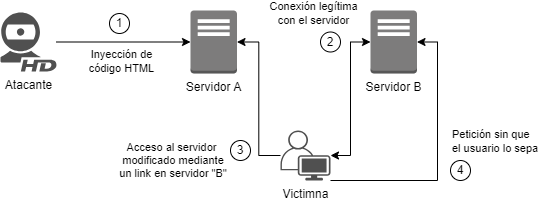
\includegraphics[width=0.9\linewidth]{fig/csrf.png}
    \caption{Ataque CSRF}
    \label{fig:csrf-attack}
\end{figure}


En el contexto de este proyecto, para mitigar este riesgo, se implementó medidas de seguridad como tokens CSRF. Estos tokens actúan como códigos secretos que deben incluirse en cada solicitud que puede realizar cambios en el estado del servidor (POST, PATCH, PUT, DELETE) y son verificados por el servidor para garantizar la legitimidad de la solicitud, evitando así que se realicen acciones no autorizadas en nombre del usuario.


\section{App Scripts}

``Apps Script es la única plataforma con bajo nivel de codificación que agiliza y facilita la compilación de soluciones empresariales que integran, automatizan y extienden Google Workspace.

Apps Script le permite compilar con HTML, CSS y JavaScript, sin que tenga que aprender un nuevo marco de trabajo exclusivo.''\cite{appscript}.

Apps Script ofrece una variedad de funcionalidades, permitiéndote realizar:

\begin{itemize}
\item Automatizaciones
\item Creación de complementos
\item Desarrollo de funciones personalizadas
\item Creación de Web Apps Script, entre otras opciones.
\end{itemize}

\subsection{Secciones de App Script}\label{sec:mt:app-script}

Dentro del archivo script creado con Google Apps Script, encontramos varias secciones que facilitan el desarrollo y la gestión de nuestros proyectos:

\begin{itemize}
\item \textbf{Información General:} Esta sección proporciona detalles sobre el script, la posibilidad de crear copias, visualizar el uso y los alcances utilizados.
\item \textbf{Editor de Código:} La sección principal donde programamos e implementamos nuestro código.

\item \textbf{Activadores:} Aquí creamos activadores o triggers basados en eventos o tiempo para ejecutar el script.

\item \textbf{Ejecuciones:} Esta sección muestra el historial de ejecuciones, logs y resultados obtenidos.

\item \textbf{Configuración:} Contiene configuraciones avanzadas para ajustar el comportamiento de nuestro script.
\end{itemize}


\subsection{Contexto del Proyecto}

En el marco de este proyecto, se empleó Google Apps Script como una solución integral para automatizar la carga de formularios en el sistema. Además, se utilizó para desarrollar plugins que mejoran la experiencia de gestión del usuario administrador mediante un menú y una interfaz gráfica intuitiva para la configuración eficiente de opciones.



\section{Web Sockets}
Según lo desarrollado en el artículo de IONOS \cite{sockets} se explican los siguientes conceptos.

Un \textbf{socket} es un mecanismo de comunicación que permite que dos procesos en diferentes máquinas o en la misma máquina se comuniquen entre sí. En términos simples, un socket proporciona una interfaz para la comunicación entre procesos.

Un \textbf{WebSocket} es un protocolo de comunicación bidireccional en tiempo real sobre un único socket TCP. A diferencia de HTTP, que sigue un modelo de solicitud-respuesta, los WebSockets permiten la comunicación en ambas direcciones en cualquier momento.

El proceso típico para establecer una conexión WebSocket es:
\begin{itemize}
\item \textbf{Handshake (apretón de manos)}: El cliente envía una solicitud HTTP al servidor solicitando el establecimiento de una conexión WebSocket. Si el servidor acepta, se produce un “apretón de manos” y la conexión se actualiza a WebSocket.

\item \textbf{Comunicación bidireccional}: Después del “apretón de manos”, ambas partes pueden enviar y recibir datos de manera bidireccional en tiempo real a través del mismo socket.
\end{itemize}

\begin{figure}[h]
    \centering
    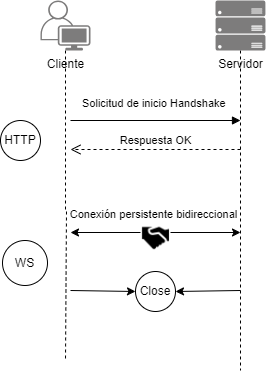
\includegraphics[width=0.5\linewidth]{fig/sockets.png}
    \caption{Web Sockets}
    \label{fig:sockets}
\end{figure}




\section{Patrón de Diseño Pub/Sub}\label{sec:pub-sub}

El patrón de diseño Publicador-Suscriptor, es una solución que permite a una aplicación comunicar eventos de manera asincrónica a múltiples consumidores interesados, evitando la necesidad de establecer una conexión directa entre los emisores y receptores. En este enfoque, un componente llamado "publicador" emite eventos a través de canales temáticos, y los "suscriptores" que están interesados en eventos específicos se registran en dichos canales.


\begin{figure}[h]
    \centering
    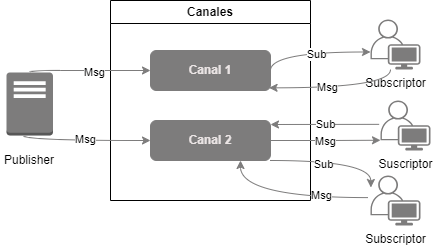
\includegraphics[width=0.8\linewidth]{fig/chanels.png}
    \caption{Publicador Suscriptor}
    \label{fig:pub-sus}
\end{figure}

En el contexto de este proyecto, se utiliza este patrón con el uso de web sockets en el sistema de notificaciones en tiempo real y actualizaciones de vistas.

\section{Docker Swarm}
\textbf{Docker} es una plataforma de código abierto diseñada para facilitar la creación, implementación y ejecución de aplicaciones en entornos aislados llamados "contenedores". Estos contenedores son unidades ligeras y portátiles que contienen todo lo necesario para que una aplicación se ejecute, incluidas bibliotecas, dependencias y código, de manera eficiente y coherente en cualquier entorno que admita Docker.

\textbf{Docker Swarm} es una herramienta de orquestación integrada en Docker que facilita la administración y escalabilidad de aplicaciones distribuidas que se ejecutan en contenedores Docker. Swarm permite la creación y administración de clústeres de Docker, donde múltiples nodos pueden trabajar juntos para proporcionar una plataforma robusta y escalable para la implementación de aplicaciones en contenedores.



\section{Normalización de la Base de Datos}

La normalización de una base de datos es un proceso esencial en el diseño de sistemas de gestión de bases de datos. 
Cabe destacar que cada forma normal depende de que se cumpla la forma normal anterior. Esto asegura que el proceso de normalización sea progresivo y que cada nivel proporcione una mayor reducción de redundancia y una mejora en la organización de los datos.
A continuación, se describen las formas normales principales:

\subsection{Primera Forma Normal (1FN)}

La 1FN elimina los grupos repetidos de las tablas individuales. En otras palabras, cada celda de la tabla debe contener un único valor atómico, evitando así la repetición de grupos de datos.

\subsection{Segunda Forma Normal (2FN)}

La 2FN establece que, si un atributo no forma parte de la clave primaria, debe proporcionar un hecho que dependa de la clave completa. Esto elimina dependencias parciales y contribuye a una mejor organización de los datos.

\subsection{Tercera Forma Normal (3FN)}

La 3FN va un paso más allá y elimina los campos que no dependen directamente de la clave primaria. Esto ayuda a asegurar que cada campo en una tabla contribuya únicamente a la información específica de esa clave.

\subsection{Forma Normal de Boyce-Codd (FNBC)}

La Forma Normal de Boyce-Codd (FNBC) es una extensión de la 3FN. Si no existen claves candidatas compuestas, una tabla se considera en FNBC. Sin embargo, si hay claves candidatas compuestas con un elemento común, puede no estar en FNBC, a menos que cada determinante en las dependencias funcionales sea una clave candidata.

\section{Propiedades ACID en Bases de Datos}

En el contexto de bases de datos, las propiedades ACID son fundamentales para garantizar la integridad y confiabilidad de las transacciones.

\begin{itemize}
  \item \textbf{Atomicidad (A):} Asegura que una transacción se realice de manera completa o no se realice en absoluto.

  \item \textbf{Consistencia (C):} Garantiza que la base de datos pase de un estado válido a otro válido después de que una transacción se haya completado.

  \item \textbf{Aislamiento (I):} Asegura que las transacciones en ejecución sean independientes entre sí, de modo que el resultado de una transacción no afecte el resultado de otras transacciones concurrentes.

  \item \textbf{Durabilidad (D):} Garantiza que una vez que una transacción se ha completado con éxito, sus cambios son permanentes y persisten incluso en caso de fallo del sistema.
\end{itemize}

    \chapter{Gestión de las Configuraciones}
\label{cap:estadoDelArte}

\section{Introducción}
En este capítulo se presenta el plan de gestión de configuraciones para el sistema de automatización y gestión del Patrocinio Jurídico de la UBA. El objetivo principal es dar a conocer las políticas, estrategias y métodos empleados para mantener la integridad del proyecto, mejorar su desarrollo y garantizar un producto de calidad.


\section{Herramientas para la Administración de Configuraciones}
En esta sección se describen las herramientas y procesos utilizados para gestionar las configuraciones del proyecto. La Tabla~\ref{tabla:gestionConfiguraciones} resume las principales herramientas y sus propósitos.


\begin{table}[h]
  \renewcommand{\arraystretch}{1.5}  % Ajuste del espacio vertical entre filas
  \begin{tabular}{p{0.4\linewidth}p{0.5\linewidth}}
    \toprule
    \textbf{Herramienta/Proceso} & \textbf{Propósito} \\
    \midrule
    Visual Studio Code & Editor de código fuente \\
    GitHub & Control de versiones y gestión de cambios \\
    Jira Software & Administración de tareas y defectos \\
    GitHub Actions & Integración continua \\
    Google Drawio & Creación de diagramas UML \\
    Mockflow  &   Creación de prototipos GUI \\
    Docker & Contenerización de servicios y aplicaciones \\
    Docker Swarm & Orquestación de contenedores \\ 
    Apps Script & Automatización y generación de extensiones para Google Forms \\
    Overleaf & Documentación en Latex \\
    Conda   & Creación de entornos virtuales en desarrollo \\
    Confluence & Documentación y registros internos \\
    \bottomrule
  \end{tabular}
  \caption{Herramientas para la administración de configuraciones}
  \label{tabla:gestionConfiguraciones}
\end{table}


\section{Herramienta de Control de Versiones}

\subsection{Dirección de Acceso}\label{sec:repo-git}
La herramienta de control de versiones utilizada en este proyecto es GitHub. El acceso al repositorio se realiza a través del siguiente enlace:


\hyperlink{https://github.com/orgs/proyecto-patrocinio/repositories}{Repositorio}


\subsection{Plan del Esquema de Ramas}
Se establece el siguiente plan para el esquema de ramas:


\begin{figure}[h]
    \centering
    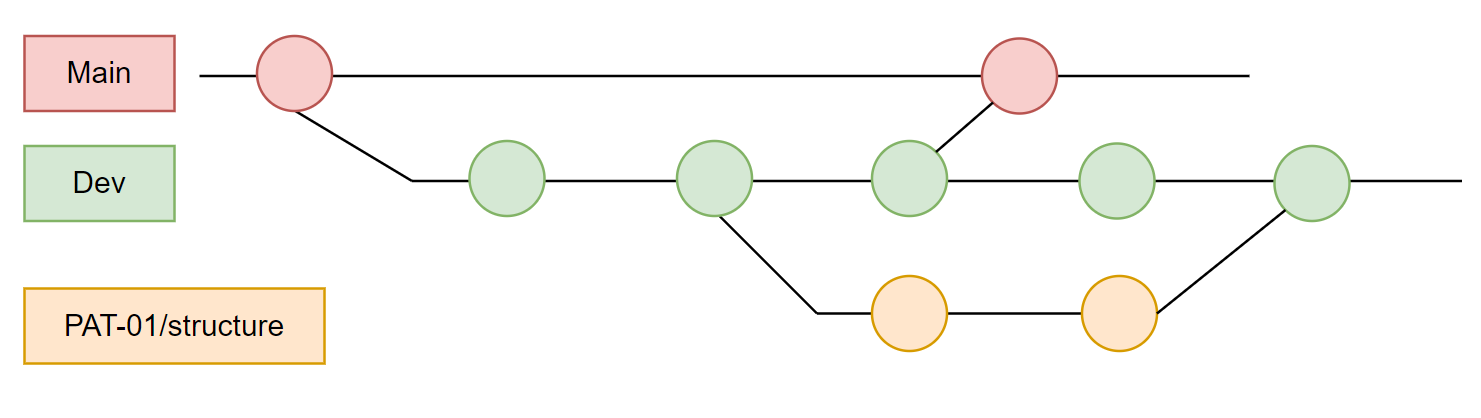
\includegraphics[width=1\linewidth]{fig/branches.png}
    \caption{Ramas de Git}
    \label{fig:enter-label}
\end{figure}


- \textbf{Principal (Main)}: Rama principal del proyecto, refleja la versión estable y funcional del código.
  
- \textbf{Desarrollo (Dev)}: Rama de desarrollo, donde se integran las nuevas características y mejoras.

- \textbf{Funcionalidades (PAT-***)}: Ramas temporales para el desarrollo de características específicas, fusionadas con la rama de desarrollo al completarse.
Esta rama consta del código la issue en Jira seguido de un slash '/' y una breve descripción en inglés. Ejemplo: \textit{PAT-01/structure\_directory}.

Las ramas Feature o funcionalidades utilizan la rama develop como rama primaria. Cuando una feature está terminada, se fusiona con la rama Dev. Las features no deben interactuar nunca directamente con Main.

\subsection{Normas de Etiquetado y de Nombramiento de los Archivos}

Las versiones se numeran con la siguiente nomenclatura \textbf{MAYOR.MENOR.PATCH}
\begin{itemize}
    \item \textbf{PATCH}: Aumenta sólo cuando se corrigen errores o se realiza un refactor que no afecta al funcionamiento, es decir, no realizan cambios en el comportamiento.
    \item \textbf{MENOR}: Se incrementa cuando se añade una nueva funcionalidad compatible con la versión anterior, si algún método se marca como obsoleto debe aumentarse la versión menor.
    \item \textbf{MAYOR}: Se incrementa cuando se produce un cambio que es incompatible con alguna versión anterior, pueden incluir cambios menor y patch.
\end{itemize}


\subsection{Políticas de Fusión de Archivos y Etiquetado en Conformidad con el Progreso de Calidad en los Entregables}

A continuación, se detallan las políticas establecidas para la gestión de versiones y el control de calidad en el proceso de desarrollo de software:

\begin{itemize}
\item \textbf{Control de Versiones en Main:} Únicamente se permitirá la inclusión de versiones en producción en la rama principal (Main).

\item \textbf{Numeración de Versiones en Releases:} En cada release, se procederá a modificar el primer número de la versión para reflejar cambios significativos. Esta práctica facilita la identificación y comprensión de las actualizaciones.

\item \textbf{Etiquetado de Versiones:} Cada versión debe ser etiquetada, proporcionando una referencia clara y accesible para su seguimiento. Este etiquetado permitirá una identificación rápida y precisa de los puntos de lanzamiento.

\item \textbf{Integración con Pruebas:} Únicamente se autorizará la fusión de código que haya superado satisfactoriamente las pruebas correspondientes. Esta medida garantiza la estabilidad y calidad del código integrado en la rama principal.

\item \textbf{Estándar de Commits Semánticos:} Cada commit que se envíe debe cumplir con el estándar de commits semánticos establecido. Este enfoque proporciona una estructura clara y consistente en los mensajes de commit, facilitando la comprensión del historial de cambios.

\end{itemize}


\subsection{Convención de Commits y Merge Request}

Para mantener un estándar, se hace uso de commits semánticos. Estos siguen la siguiente estructura:

\texttt{PREFIX(CODE): DESCRIPTION}

\textbf{Ejemplo para commits:}
feat(PAT-05): Add function to search for files

\textbf{Ejemplo para merge request:}
feat[PAT-05]: Add Calendar

Puede ver un ejemplo en el siguiente link \href{https://github.com/proyecto-patrocinio/proyecto-patrocinio/pull/100}{Merge Request}.

A continuación se listan los posibles prefijos:

\begin{itemize}
    \item \texttt{feat}: Una nueva característica para el usuario.
    \item \texttt{fix}: Arregla un bug que afecta al usuario.
    \item \texttt{imp}: Cambios que mejoran el funcionalidades o rendimientos.
    \item \texttt{build}: Cambios en las tareas de despliegue o instalación.
    \item \texttt{docs}: Cambios en la documentación.
    \item \texttt{refactor}: Refactorización del código como cambios de nombre de variables o funciones.
    \item \texttt{test}: Añade tests o refactoriza uno existente.
\end{itemize}



\section{Estructura de Directorios}\label{sec:estr-directory}

El diseño del proyecto se organiza en tres repositorios principales alojados en GitHub, cada uno cumpliendo un rol específico en la implementación y gestión del sistema. A continuación, se detallan estos repositorios junto con sus respectivos enlaces:

\begin{itemize}
    \item \textbf{proyecto-patrocinio} [\href{https://github.com/proyecto-patrocinio}{GitHub-unit}]: Este repositorio alberga tanto el núcleo del proyecto como su interfaz de usuario. Se estructura en carpetas específicas para el backend, frontend y archivos de script destinados a Google App Script.
    
    \item \textbf{cms-deploy} [\href{https://github.com/proyecto-patrocinio/cms-deploy}{GitHub-deploy}]: Este repositorio se centra en la orquestación y configuración del despliegue de la plataforma mediante Docker Swarm. Contiene archivos de composición para Docker, plantillas y configuraciones necesarias para asegurar un despliegue efectivo.
    
    \item \textbf{cms-docs} [\href{https://github.com/proyecto-patrocinio/cms-docs}{GitHub-docs}]: Aquí se encuentra toda la documentación del proyecto. Este repositorio incluye información detallada sobre la arquitectura del sistema, sus componentes, guías de instalación y uso, entre otros documentos esenciales para el desarrollo y mantenimiento del proyecto.

    \item \textbf{cms-test} [\href{https://github.com/proyecto-patrocinio/cms-test}{GitHub-test}]: En este repositorio se encuentran los test de sistema. Éste se utiliza en el proceso de verificación y validación del software para garantizar la calidad del mismo.
\end{itemize}

\subsection{Repositorio \textit{cms-deploy}}\label{subsec:directory-deploy}

El repositorio \textit{cms-deploy} se encarga específicamente de la configuración de despliegue. Incluye archivos de composición para Docker Swarm, plantillas y configuraciones necesarias para garantizar un despliegue eficiente y escalable (ver Figura \ref{fig:deploy-directory}).


En la raíz del directorio, destaca el archivo de composición para Docker Swarm, que define el stack de contenedores. Además, se encuentra la carpeta \texttt{resources}, que contiene archivos de configuración y variables de entorno para los contenedores. La subcarpeta \texttt{templates} dentro de \texttt{resources} se subdivide en dos directorios: \texttt{account} y \texttt{notifications}. El directorio \texttt{account} almacena plantillas HTML relacionadas con los correos electrónicos enviados para el registro de cuentas y cambios de contraseñas. Por otro lado, en el directorio \texttt{notifications}, se encuentran los archivos HTML que se enviarán por correo electrónico para notificar las solicitudes de casos a las comisiones, así como las respuestas a estas solicitudes. 


\begin{figure}[H]
    \centering
    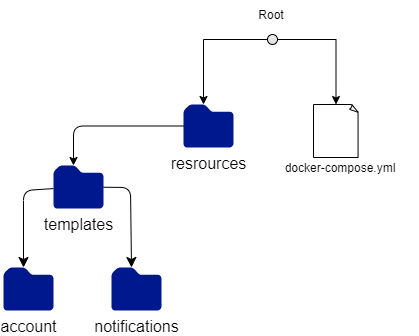
\includegraphics[width=0.5\linewidth]{fig/deploy-directory.png}
    \caption{Estructura de directorios del repositorio \textit{cms-deploy}.}
    \label{fig:deploy-directory}
\end{figure}

\subsection{Repositorio \textit{cms-docs}}

En el repositorio \textit{cms-docs}, se concentra toda la documentación del proyecto. Desde detalles técnicos hasta guías de usuario, este repositorio actúa como una fuente centralizada de información para desarrolladores, administradores y usuarios finales.

\subsection{Repositorio \textit{cms-test}}
En el repositorio \textit{cms-test}, se encuentran todos los casos de prueba automatizados realizados con Robot Framework y Selenium.

\begin{figure}[H]
\centering
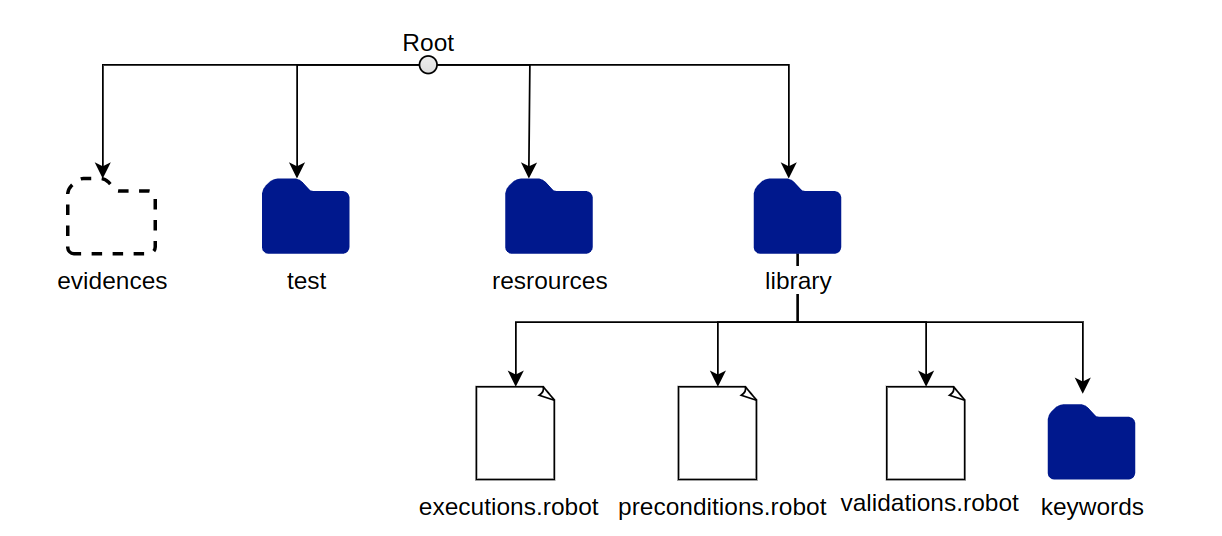
\includegraphics[width=0.9\linewidth]{fig/test-directory.png}
\caption{Estructura del directorio de pruebas en \textit{cms-test}.}
\label{fig:test-directory}
\end{figure}

Dentro del directorio \textit{test}, se ubican los casos de prueba específicos. En el directorio \textit{resources} se almacenan los archivos utilizados en las pruebas. En el directorio \textit{library}, se encuentra la implementación de las \textit{keywords}, divididas en tres archivos: \textit{preconditions.robot}, \textit{executions.robot} y \textit{validations.robot}. Cada archivo contiene las \textit{keywords} relacionadas con las precondiciones (Given), acciones (When) y validaciones (Then) respectivamente. Por otro lado, en la carpeta \textit{keywords}, se agrupan las \textit{keywords} con la lógica para realizar diversas tareas.

Por último, la carpeta \textit{evidences} se genera automáticamente después de ejecutar los tests, en la cual se recopilan las evidencias generadas para cada caso de prueba.

\subsection{Repositorio \textit{proyecto-patrocinio}}

El repositorio \textit{proyecto-patrocinio} constituye el núcleo esencial del proyecto, integrando tanto el backend como el frontend, junto con los scripts para Google App Script.

A continuación, se presenta una representación visual de la estructura de directorios específica del repositorio \textit{proyecto-patrocinio}, ofreciendo una visión detallada de la distribución de archivos y carpetas clave para comprender la organización del código y los recursos del proyecto (ver Figura \ref{fig:unit-directory}).

\begin{figure}[h]
    \centering
    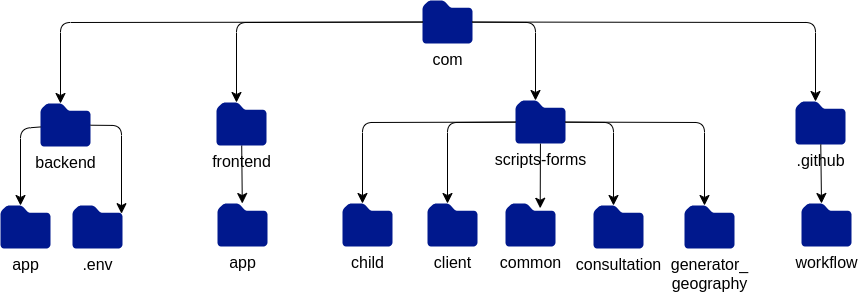
\includegraphics[width=1\linewidth]{fig/directory.png}
    \caption{Estructura de directorios del repositorio \textit{proyecto-patrocinio}.}
    \label{fig:unit-directory}
\end{figure}

Dentro del directorio \texttt{backend}, se encuentran dos carpetas principales: \texttt{.env}, que alberga todas las variables de entorno configurables, y \texttt{app}, donde se desarrolla la API REST en Django. Este último contiene toda la lógica de negocio de la plataforma.

En el directorio \texttt{frontend}, la carpeta \texttt{app} almacena la interfaz de usuario Reactiva, con una mínima lógica necesaria para obtener y visualizar datos.

La carpeta \texttt{scripts-forms} se subdivide en cinco directorios. \texttt{Child} contiene scripts y archivos necesarios para el formulario de registro de un nuevo hijo para un cliente existente. \texttt{Client} incluye scripts y archivos para el formulario de registro de un nuevo cliente. \texttt{Consultation} alberga scripts y archivos para el formulario de creación de una nueva consulta a un cliente existente. La carpeta \texttt{common} contiene archivos compartidos por los formularios mencionados anteriormente. La carpeta \texttt{generator-geography} incluye la hoja de cálculo y scripts necesarios para generar nacionalidades, provincias y localidades en los cuestionarios de los formularios mencionados.

Dentro del directorio \texttt{.github}, la carpeta \texttt{workflows} contiene los pipelines para la integración continua del proyecto. Esta configuración garantiza una gestión eficiente del desarrollo y la implementación continua del proyecto.


\section{Herramientas de Gestión de Tareas y Defectos}

Para la supervisión y gestión eficiente de tareas y defectos, se empleó JIRA (\href{https://prietojulii.atlassian.net/jira/software/projects/PAT/boards/1}{Link Jira}). Esta plataforma proporciona tanto el backlog como el board del sprint activo, ofreciendo una vista integral del progreso del proyecto. JIRA no solo facilita la asignación y seguimiento de tareas, sino que también ofrece una interfaz interactiva que simplifica la colaboración y la toma de decisiones. 

\subsection{Confluence}
La integración con Confluence añade un valor adicional al proceso de gestión. Con la capacidad de agregar páginas Markdown directamente al proyecto, se promueve la documentación detallada y la contextualización de las issues. Esto no solo mejora la comprensión de los problemas abordados, sino que también facilita la colaboración al proporcionar un contexto más amplio para la toma de decisiones.

\subsection{Issues}
Cada Issue consta de:
\begin{itemize}
    \item Una descripción detallada.
    \item Un etiquetado que indica el tipo de problema (bug, feat, task).
    \item Un enlace directo a Commits y Merge Request/rama asociados. Para establecer conexiones efectivas entre la Issue, los commits y los Merge Requests o ramas, es esencial agregar el código de la Issue en cada uno de ellos.
    \item Una asignación a persona responsable de hacer avanzar el problema.
    \item Comentarios de cualquier persona con acceso a Jira.
    \item Épica a la cual pertenece.
\end{itemize}
Se ilustra un ejemplo en el siguiente enlace: \href{https://prietojulii.atlassian.net/browse/PAT-44}{Link a la ISSUE}.

\subsection{Épicas}
En el ámbito de la gestión de proyectos, una épica se refiere a una categoría o tema amplio que engloba un conjunto de tareas o historias de usuario relacionadas.
En el contexto de este proyecto, se han identificado diversas épicas que se especifican a continuación.


\subsubsection{Calendario}
Se centra en la integración de calendarios, programación de eventos y cualquier otra característica asociada al seguimiento temporal de los casos.

\subsubsection{Documentación}
Abarca actividades destinadas a mejorar la comprensión y el mantenimiento del proyecto. Incluye la configuración de logs para facilitar la monitorización y depuración del sistema, la actualización regular de los archivos README para proporcionar información actualizada y relevante, el refinamiento y ampliación de las docstrings en el código fuente para mejorar la comprensión de las funciones y métodos, la elaboración de documentación técnica detallada que explique la arquitectura, diseño y decisiones técnicas del proyecto, la creación y actualización de manuales de usuario que guíen a los usuarios finales sobre el uso efectivo del sistema, y la generación de informes detallados que aborden aspectos específicos del proyecto.

\subsubsection{Testing}
Se enfoca en la implementación y mejora de pruebas para garantizar la calidad del software. En este proyecto, la atención se centra principalmente en dos aspectos: pruebas unitarias de backend y frontend, y pruebas de sistema.

\subsubsection{Infraestructura}
Se enfoca en la gestión y mejora de los recursos tecnológicos subyacentes del proyect. Las tareas dentro de esta épica se dividen en dos aspectos clave:

\textbf{Desarrollo de Pipelines:} Se realiza el diseño, desarrollo y optimización de pipelines que automatizan procesos relacionados con la implementación de integración y entrega continua del proyecto.

\textbf{Despliegue en Docker Swarm:} Se establecen y mejoran los procedimientos de despliegue de la aplicación en el entorno Docker Swarm. 



\subsubsection{Notificaciones}
Aborda la implementación de sistemas de notificación eficientes. Esto incluye alertas y correos electrónicos que informe sobre eventos relevantes en el sistema.

\subsubsection{Comentarios}
Se dedica a la implementación de la funcionalidad de comentarios dentro de las consultas, incluyendo la carga de documentos.

\subsubsection{Panel de Control}
Se centra en la creación de las páginas de panel de control, el cual consta de tablas para visualizar los datos y descargarlos.

\subsubsection{Integración con Google Forms}
Busca facilitar la conexión y utilización de formularios de Google dentro del proyecto. Esto implica la automatización de la recopilación de datos y la integración de formularios en procesos específicos.

\subsubsection{Administración}
Se centra en la implementación de la administración básica como el registro de usuarios, gestión de permisos y la carga de datos iniciales al sistema.

\subsubsection{Consultorio}
Abarca las tareas vinculadas a la creación de un tablero de consultoría. Este tablero tiene como objetivo gestionar los casos judiciales y facilitar el proceso de envío de casos a las comisiones correspondientes para su patrocinamiento. Se centra en la implementación de funcionalidades específicas que agilizan y optimizan la administración de casos, desde su registro inicial hasta su asignación a las comisiones pertinentes.

\subsubsection{Tablero}
Engloba las tareas relacionadas con la creación y desarrollo de un tablero destinado a la comisión. Este tablero tiene como objetivo fundamental la gestión integral de casos, incluyendo su ingreso, su seguimiento, y la organización eficiente de cada uno de ellos dentro del sistema. Se enfoca en la implementación de funcionalidades clave que permiten a la comisión llevar a cabo sus responsabilidades de manera efectiva, proporcionando una interfaz intuitiva y completa para la administración de los casos asignados.


\subsubsection{Seguridad y Privacidad}
Se dedica a fortalecer la seguridad y privacidad del sistema. Incluye la implementación de medidas de seguridad, la gestión de accesos y la protección de datos.



\section{Herramienta de Integración Continua}

\textbf{GitHub Actions} es una poderosa plataforma de Integración Continua y Despliegue Continuo (CI/CD) que posibilita la automatización de pipelines para la construcción, prueba y despliegue de proyectos. A través de GitHub Actions, se pueden crear flujos de trabajo personalizables que se encargan de compilar y probar cada pull request enviado al repositorio, así como desplegar las contribuciones fusionadas en la rama principal hacia los entornos de producción.

Un \textbf{WorkFlow} o flujo de trabajo es un proceso automatizado configurable que ejecuta uno o más trabajos (jobs). Estos flujos de trabajo se definen mediante un archivo de configuración YAML que se incorpora al repositorio. La ejecución del flujo de trabajo puede desencadenarse por eventos específicos dentro del repositorio, como cambios en el código, pull requests, o de manera manual.

En el contexto de este proyecto, se han empleado dos flujos de trabajo, uno dedicado al frontend y otro al backend, alojados en el repositorio \textit{proyecto-patrocinio} (ver \ref{sec:estr-directory}).

Para ambos pipelines, se establecen disparadores que inician el flujo de trabajo compuesto por dos etapas principales: \texttt{ci} y \texttt{cd}.

- \textbf{\texttt{triggers}:} La ejecución de los pipelines se configura en respuesta a eventos específicos. Estos eventos incluyen el lanzamiento de una nueva versión (\textit{release}) o la realización de un \textit{push} a las ramas \texttt{main} o \texttt{dev}. En el caso de las ramas \texttt{dev} o \texttt{main}, los pasos del flujo presentan una ligera variación para adecuarse a la gestión de versiones y etiquetas de las imágenes destinadas a Docker Hub.

- \textbf{\texttt{ci}:} Este trabajo realiza un conjunto de pasos esenciales, incluyendo la verificación de la calidad del código, la configuración del entorno de la API, la instalación de dependencias, y la ejecución de pruebas, entre otros. Garantiza que el código enviado cumpla con los estándares definidos antes de proceder con la siguiente etapa.

- \textbf{\texttt{cd}:} La etapa de entrega continua se activa tras el éxito de la etapa de integración continua (\texttt{ci}). En esta fase, se realiza la construcción y la publicación de la imagen de Docker en Docker Hub. La imagen se etiqueta con la versión actual y la etiqueta "latest". Este proceso permite que la imagen esté lista para ser implementada en entornos de producción.



\begin{figure}[h]
    \centering
    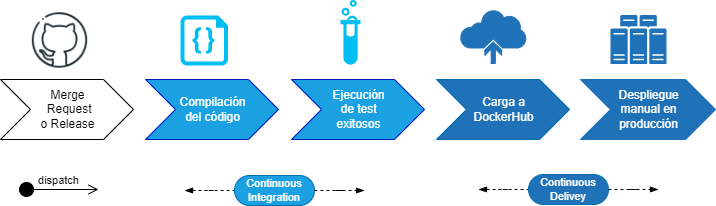
\includegraphics[width=1\linewidth]{fig/cicd.png}
    \caption{CI/CD}
    \label{fig:ci-cd}
\end{figure}

Consulte la sección \href{https://github.com/proyecto-patrocinio/proyecto-patrocinio/actions}{GitHub Actions} del repositorio para ver los detalles de los reportes.




\section{Formato de Entrega}
La entrega del proyecto se realizará vía email adjuntando los siguientes archivos:

\begin{itemize}
    \item Un archivo comprimido denominado \texttt{cms-deploy.zip}, que abarca los componentes esenciales para el despliegue del proyecto.
    \item La documentación en formato PDF.
    \item Un archivo comprimido \texttt{proyecto-patrocinio.zip}, que contiene la unidad del proyecto.
\end{itemize}

Además, se proporcionarán los nombres de las imágenes correspondientes al backend y frontend.




\section{Tablero de Control de Configuración - CCB}

El Change Control Board (CCB), o Tablero de Control de Configuración en español, desempeña un papel crucial en la supervisión y evaluación de los cambios propuestos en la configuración del sistema, asegurando la implementación de modificaciones de manera estructurada y controlada.


\subsection{Metodología Ágile}
La elección del marco de trabajo SCRUM se fundamentó en la idoneidad de su enfoque ágil, especialmente en proyectos con requisitos no completamente definidos. SCRUM ofrece una estructura que favorece el progreso incremental a través de sprints y se ajusta bien a la gestión de tareas en entornos dinámicos.

La implementación de SCRUM en este proyecto requirió adaptaciones específicas debido al contexto particular de este proyecto. Se realizaron sprints con una duración flexible de 2 a 4 semanas, ajustando el tiempo según la disponibilidad durante el año lectivo. Adicionalmente, se programaron reuniones de revisión y planificación al final y al inicio de cada sprint, respectivamente, para evaluar avances y definir las metas para el próximo ciclo.

Además, se optó por simplificar los roles de Product Owner, Scrum Master y Developer considerando las limitaciones de recursos de personal.



\subsection{Miembros y Funciones}
A continuación se tabulan los roles de los miembros del proyecto (ver \ref{tab:ccb}).

\begin{table}[h]
    \centering
    \begin{tabular}{|c|p{5cm}|p{4cm}|}
        \hline
        \textbf{Rol} & \textbf{Función} & \textbf{Responsable} \\
        \hline
        Directores del proyecto
        & Revisión del proyecto. Aprobación de decisiones importantes. Gestiona el buen funcionamiento del proyecto, quien controla y administra los recursos (tanto personales como económicos) con el fin de cumplir el plan y el objetivo definido. Se encargan de que todo funcione según lo establecido, resolver desviaciones en el plan, y hacer que los diferentes equipos del proyecto se sincronicen y trabajen juntos.
        & Director, Danilo Paez y Co-directora, Laura Díaz \\
        \hline
        Stakeholder
        & Son fuente de información para el Equipo de Scrum. Tomadores de decisiones  internos de la organización.
        & Carina Papini y Melina Raban \\
        \hline
        Asesor/Consultor
        &  Proporciona asesoramiento y orientación técnica.
        Está disponible para consultas y resolución de dudas
        relacionadas con aspectos específicos del proyecto.
        & Daniel Britos \\
        \hline
        Desarollo Full Stack e Ingeniería
        & Detección y documentación de requerimientos. Diseño y planificación del software en sprints. Encargado de tomar el control de la herramienta de gestión de defecto, documentando específicamente sobre cada problema en el que se trabaja.
        Se encargará de crear un incremento terminado a partir de los elementos del Product Backlog seleccionados por sprint.
        & Julieta Abigail Prieto\\
        \hline
    \end{tabular}
    \caption{Tablero de Miembros y Funciones}
    \label{tab:ccb}
\end{table}

Además, se realiza un reconocimiento especial a Alberto Germán Sotelo y Agustina Cuello por su colaboración como becarios del laboratorio IALAB durante la fase inicial del proyecto realizando tareas de desarrollo backend.


    \chapter{Requerimientos y Especificaciones}\label{cap:disenio}

\section{Introducción}
En este capítulo se detalla en su totalidad el producto de la plataforma de gestión y automatización para el proceso de selección de los casos del Patrocinio Jurídico Gratuito de la UBA. En este se describen sus funcionalidades, especificaciones y limitaciones en cuanto a su utilización.

\section{Alcance del Producto}
Este producto está orientado a profesores y tomadores de casos del Patrocinio Jurídico Gratuito, con el fin de facilitar y mejorar la eficiencia del sistema de solicitud y control histórico de los casos, asegurando una experiencia intuitiva en su utilización.

El alcance de esta plataforma abarca el proceso desde la recepción de datos a través de Google Forms, la integración de la información en el sistema, la gestión de los casos en la asignación a comisiones y, finalmente, el seguimiento y gestión de los casos por parte de los profesores de la comisión. 

\section{Referencias}
A continuación, se presenta una lista detallada de las tecnologías utilizadas en el desarrollo del proyecto, acompañadas de enlaces a sus respectivas documentaciones. Estos recursos fueron seleccionados estratégicamente para facilitar el desarrollo, la implementación y el mantenimiento del sistema.


\begin{table}[H]
    \centering
    \begin{tabular}{|p{11cm}|p{4cm}|}
        \hline
        \textbf{Recurso} & \textbf{Sitio Web} \\
        \hline
        Documentación de Python 3. & \href{https://docs.python.org/3/}{Python3} \\
        \hline
        Documentación de Django 4.1. & \href{https://docs.djangoproject.com/en/4.1/}{Django} \\
        \hline
        Documentación de Django Rest Framework, una extensión de Django para construir APIs. & \href{https://www.django-rest-framework.org/#quickstart}{Django-Rest} \\
        \hline
        Documentación de PostgreSQL para la base de datos. & \href{https://www.postgresql.org/docs/current/}{PostgreSQL} \\
        \hline
        Documentación Django-docutils para la automatización de la documentación de la API. & \href{https://docs.djangoproject.com/en/4.1/ref/contrib/admin/admindocs/}{Django-docutils} \\
        \hline
        Documentación del lenguaje Gherkin para listar los requerimientos. & \href{https://docs.behat.org/en/v2.5/guides/1.gherkin.html}{Gherkin} \\
        \hline
        Documentación de Nginx para un servidor web y/o proxy inverso. & \href{http://nginx.org/en/docs/}{Nginx} \\
        \hline
        Documentación de Gunicorn, un servidor HTTP Python WSGI para UNIX. &
        \href{https://gunicorn.org/#docs}{Gunicorn} \\
        \hline
        Documentación de React, una biblioteca de JavaScript para construir interfaces Reactivas de usuario. & \href{https://es.react.dev/reference/react}{React}\\
        \hline
        Documentación de Material-UI, una biblioteca de componentes de interfaz de usuario para React. & \href{https://mui.com/material-ui/getting-started/}{MUI} \\
        \hline
        Documentación de Beautiful Drag and Drop para implementar funcionalidades de arrastrar y soltar. & \href{https://github.com/atlassian/react-beautiful-dnd}{React-Beautiful-DND} \\
        \hline
        Documentación de Django Channels para el manejo de conexiones en tiempo real a Django. & \href{https://channels.readthedocs.io/en/latest/}{Channels} \\
        \hline
        Documentación de Daphne, un servidor ASGI (Asynchronous Server Gateway Interface) para aplicaciones asincrónicas con Django. & \href{https://docs.djangoproject.com/en/5.0/howto/deployment/asgi/daphne/}{Daphne}\\
        \hline
        Documentación de Docker. & \href{https://docs.docker.com/engine/}{Docker} \\
        \hline
        Documentación de Docker Swarm para la orquestación de contenedores. & \href{https://docs.docker.com/engine/swarm/}{Docker-Swarm}\\
        \hline
        Documentación de Robot Framework para la automatización de test. & \href{https://robotframework.org/robotframework/latest/RobotFrameworkUserGuide.html}{Robot-Framework}\\
        \hline
        Documentación de Selenium para la automatización de tareas desde el browser. & \href{https://robotframework.org/SeleniumLibrary/SeleniumLibrary.html}{Selenium}\\
        \hline
    \end{tabular}
    \caption{Recursos y Enlaces de Documentación}
    \label{tab:recursos_documentacion}
\end{table}



\newpage

\section{Descripción General}

\subsection{Perspectiva del Producto}
El producto surge para abordar una necesidad administrativa identificada en la organización del Patrocinio Jurídico de la UBA. Actualmente, los formularios de los solicitantes se envían automáticamente por Google Forms mediante correo electrónico y luego se cargan manualmente en un software pago, Trello. Esta metodología presenta desafíos de integración y no se ajusta completamente a los requisitos específicos de la organización. La solución propuesta busca mejorar la organización y gestión de casos mediante un software que se integre de manera eficiente con Google Forms.

El sistema se integrará sin inconvenientes con Google Forms para facilitar la captura de datos relacionados con casos judiciales y nuevos clientes. Este enfoque optimizará el proceso de solicitud, selección y gestión de casos, brindando a los usuarios finales una experiencia más sencilla y ágil. La interfaz de usuario, diseñada intuitiva y amigablemente, seguirá las mejores prácticas de diseño centrado en el usuario, asegurando eficiencia y transparencia en la experiencia del usuario.

\subsection{Funciones del Producto}
El sistema desarrollado proporciona un conjunto integral de funciones diseñadas para satisfacer las necesidades específicas de la gestión de casos judiciales y su asignación a las comisiones. Integra de manera fluida con Google Forms, permitiendo la captura eficiente de datos relacionados con casos judiciales y nuevos clientes. Facilita la selección y asignación de casos a comisiones. La interfaz de usuario intuitiva permite el seguimiento detallado de cada caso a lo largo de su ciclo de vida, facilitando una gestión efectiva y transparente por parte de los profesores de las comisiones. Incluye un sistema de notificaciones vía email y alertas para anunciar ciertos eventos. La interfaz de usuario, es intuitiva, fácil de navegar y brinda una experiencia eficiente, contribuyendo a mejorar la eficiencia, la transparencia y la efectividad en la gestión de casos y la selección de comisiones.

\subsection{Tipos de Usuarios y Características}
El sistema contempla varios tipos de usuarios, cada uno con funciones y características específicas para satisfacer sus necesidades dentro del proceso. Los roles principales incluyen:

\textbf{Administradores del Sistema}: Tienen acceso completo al sistema y la capacidad de gestionar usuarios y acceder a todas las funcionalidades. Su función principal es garantizar el correcto funcionamiento y la configuración adecuada del sistema.

\textbf{Profesores de Comisión}: Estos usuarios son responsables de revisar, evaluar y gestionar los casos asignados a su comisión. Pueden acceder a la información detallada de cada caso, realizar comentarios, asignar tareas y seguir el progreso de manera integral.

\textbf{Solicitantes}: Son los usuarios encargados de presentar casos judiciales mediante Google Forms. Aunque no tienen acceso directo a la plataforma, desempeñan un papel crucial al ingresar casos y nuevos clientes a través de Google Forms, contribuyendo así al flujo eficiente de datos en el sistema.

\textbf{Administradores de Casos}: Más conocidos como \textbf{Tomadores de Caso}, este rol se ocupa de la gestión específica de los casos, desde su recepción hasta su asignación a una comisión. Pueden revisar la información proporcionada por los solicitantes y asignar casos a las comisiones correspondientes.




\subsection{Entorno Operativo}

La plataforma estará diseñada para operar en un entorno que cumpla con los siguientes requisitos:

\subsubsection{Requisitos de Servidor}
La aplicación está diseñada para ser accesible desde cualquier dispositivo con capacidad para ejecutar contenedores Docker, lo que incluye sistemas operativos como Linux, Windows y macOS.

Se recomienda empezar al menos con:
\begin{itemize}
    \item 100 GB de almacenamiento libre
    \item 6 GB de RAM
    \item 2 núcleo de CPU
\end{itemize}

Estos requisitos proporcionarán una base para el despliegue inicial de la aplicación, asegurando un funcionamiento estable y eficaz. Se debe tener en cuenta que estos son requisitos mínimos y se puede considerar la posibilidad de aumentar estos recursos en función de la carga de trabajo y el crecimiento futuro de la aplicación.

\subsubsection{Navegadores Soportados}

\begin{itemize}
    \item Google Chrome. Se probó en la versión Versión 120.0.6099.130.
    \item Mozilla Firefox. Se probó en la versión 121.0.
\end{itemize}

\subsubsection{Conectividad}
Se requiere una conexión a Internet estable para el correcto funcionamiento de la integración con Google Forms y el acceso a la plataforma. La velocidad de la conexión afectará directamente la eficiencia en la carga y manejo de datos.

\subsubsection{Dispositivos Compatibles}
La plataforma está diseñada para ser accesible desde dispositivos con pantallas de tamaño mediano a grande, como computadoras de escritorio, laptops y tabletas. El acceso desde dispositivos móviles puede ser posible, pero la experiencia de usuario puede variar según el tamaño de la pantalla.




\section{Restricciones de Diseño e Implementación}
\begin{itemize}
    \item \textbf{Limitaciones a nivel de Interfaz}:  Se busca una interfaz gráfica simple e intuitiva que sea      semejante a la interfaz de Trello la cual, los usuarios finales están familiarizados. Para así facilitar la utilización para usuarios con pocos conocimientos en el ámbito de la informática.
    \item \textbf{Limitaciones presupuestarias}: Debido a que el organismo solicitante del producto no tiene presupuesto para la creación y mantenimiento del sistema. Este debe tener un costo bajo o nulo.
    \item \textbf{Seguridad y Privacidad}
    La plataforma debe seguir las mejores prácticas de seguridad para proteger la información confidencial de los casos judiciales y los datos de los usuarios. Se deben implementar mecanismos de autenticación y autorización, y se debe garantizar el cifrado de la comunicación entre el cliente y el servidor.
\end{itemize}


\section{Modelo Conceptual de Datos - DER}

En la construcción del Modelo Conceptual de Datos, se tomó la decisión de utilizar PostgreSQL como motor de búsqueda para la base de datos, basándonos en su destacada capacidad para respaldar las propiedades fundamentales del modelo ACID (Atomicidad, Consistencia, Aislamiento y Durabilidad). Estas características son esenciales para garantizar la integridad y confiabilidad de las transacciones en la base de datos.

Posteriormente, al interpretar la matriz de relaciones, se simplificó la visualización al omitir algunas tablas intermedias, para facilitar la comprensión del esquema general de la base de datos de manera más accesible.

Los diagramas subsiguientes se derivan de un modelo de base de datos que ha sido procesado y refinado hasta alcanzar la tercera forma normal, una práctica común con el propósito de optimizar la organización y estructura de los datos, evitando redundancias y asegurando consistencia.

Adicionalmente, como estrategia para simplificar el diseño y reducir la complejidad asociada al manejo de grandes volúmenes de datos, se ha decidido tratar las calles como cadenas de texto independientes de las localidades. Esta decisión se basa en la idea de no vincularlas geográficamente, evitando así la carga adicional que implicaría gestionar todas las calles de Argentina, la cual podría resultar significativa en términos de volumen de datos y complejidad operativa.

Consulte en el anexo, los Diagramas~\ref{mat:der}, \ref{mat:der2} y \ref{mat:der3} para visualizar las matrices de relaciones de entidades.



A continuación se presenta el diagrama de Entidad-Relación. En celeste se resalta la relación muchos a muchos, la cual ha sido reemplazada por una tabla intermedia denominada "board-user". Y en un azul mas oscura se representa la herencia de Person con User y Client.

\begin{figure}[H]
    \centering
    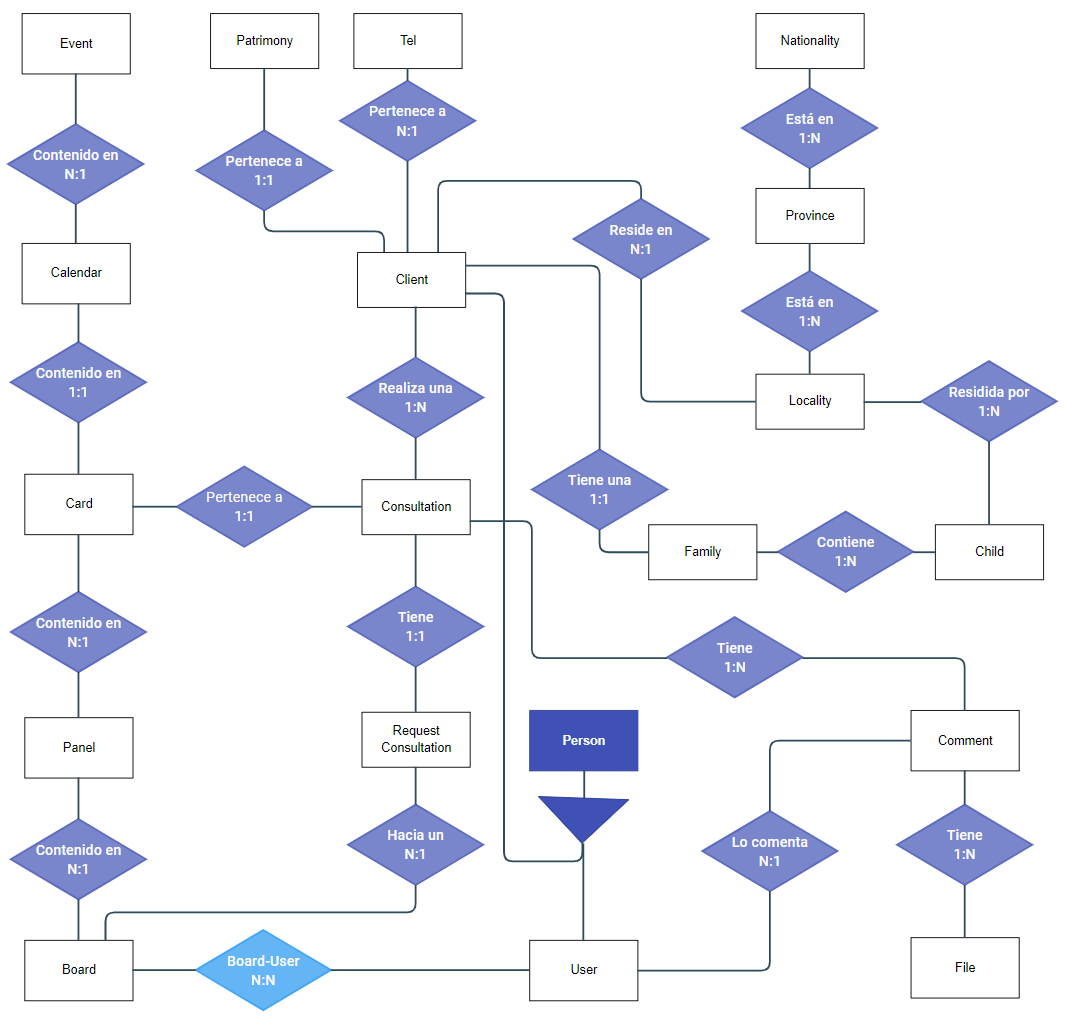
\includegraphics[width=1\linewidth]{fig/der.png}
    \caption{Diagrama Entidad Relación}
    \label{fig:der}
\end{figure}

\newpage

La implementación del modelo se lleva a cabo en Django. Sin embargo, para simplificar la explicación, se han omitido otras entidades relacionadas al usuario propias de Django, como tokens, grupos, etc. A continuación, se presenta el resultado visualizado mediante DBeaver, utilizado como gestor de la base de datos.

\begin{figure}[H]
    \centering
    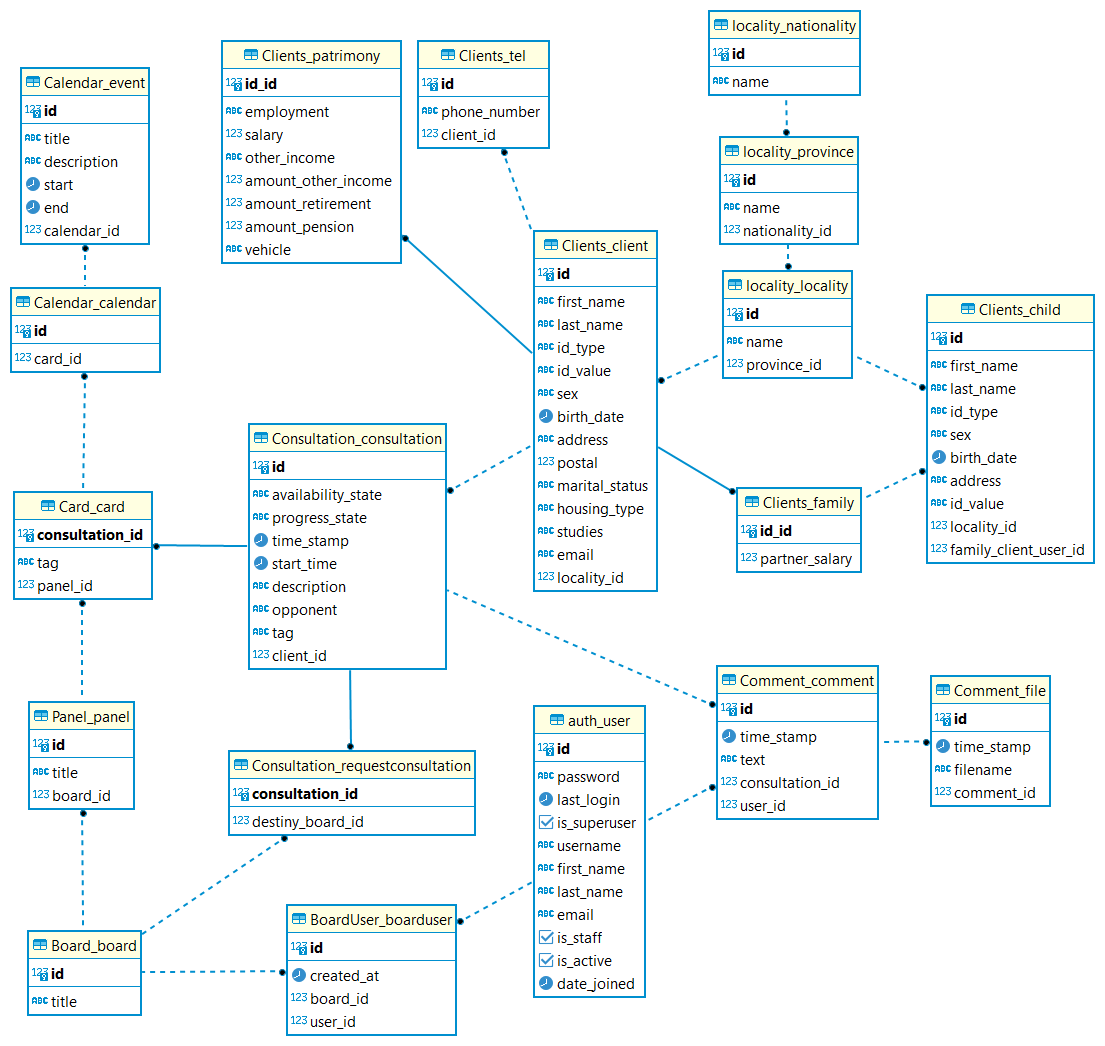
\includegraphics[width=1\linewidth]{fig/dbeaver.png}
    \caption{Implementación del Modelo Entidad Relación}
    \label{fig:dbeaver}
\end{figure}




\section{Requerimientos de Interfaces Externas}


En esta sección, se presenta los requerimientos de de Interfaces, que sirve como un elemento para la visualización y estructuración de la interfaz de usuario. A continuación, se exhiben los mockup representativos del diseño propuesto para la interfaz gráfica de usuario (GUI).

\subsection{Consultoría}

La Figura \ref{fig:gui-consultancy} exhibe un mockup que encapsula la apariencia y disposición previstas de la interfaz de usuario, específicamente en el contexto de la funcionalidad de consultoría.

Dada la necesidad de lograr una experiencia intuitiva, se estableció como requisito la implementación de tableros para la asignación de casos, tomando como referencia la utilización previa de Trello en el organismo.

\begin{figure}[h]
\centering
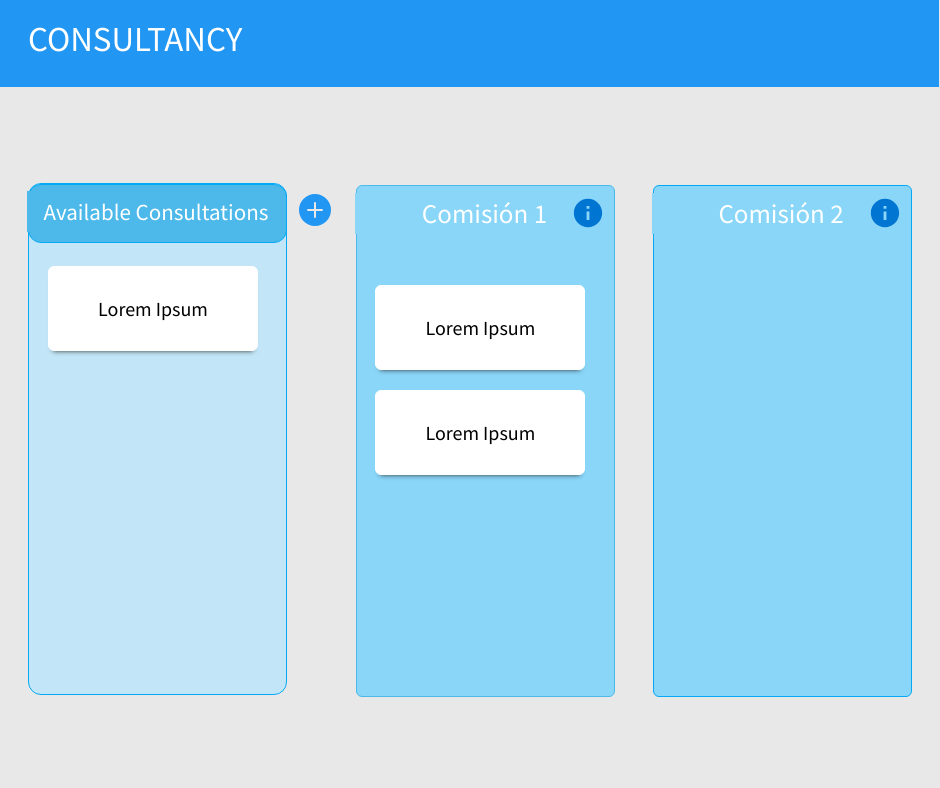
\includegraphics[width=1\linewidth]{fig/GUI-consultancy.png}
\caption{Mockup de la Interfaz Gráfica de Usuario (GUI) para la Página Consultoría}
\label{fig:gui-consultancy}
\end{figure}


A la izquierda, se ubica el tablero de casos sin asignar, mientras que a la derecha se presentan los tableros destinados para enviar las solicitudes de asignación del caso a las diversas comisiones. Cada tarjeta (card) en estos tableros representa una consulta específica.

Adicionalmente, se incorporan dos elementos clave para la interacción:
\begin{itemize}
    \item El botón ``+''  facilita la creación de nuevas consultas.
    \item El botón de información proporciona detalles específicos sobre la comisión correspondiente.
\end{itemize}



\subsection{Tablero de Trabajo para Cada Comisión}

El diseño del tablero de trabajo adopta una lógica similar a la implementada en la funcionalidad de consultoría, manteniendo paneles organizativos que permiten la manipulación intuitiva de tarjetas mediante el sistema de arrastre y soltar.


\begin{figure}[H]
\centering
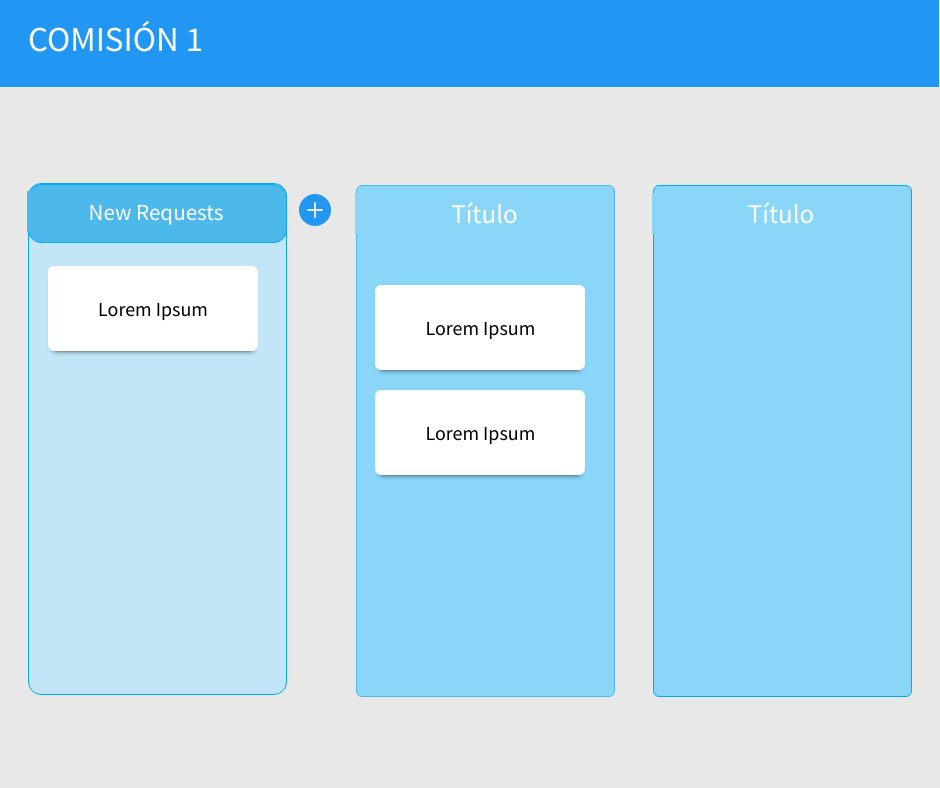
\includegraphics[width=1\linewidth]{fig/board.png}
\caption{Mockup de la Interfaz Gráfica de Usuario (GUI) para el Tablero de Comisión}
\label{fig:board}
\end{figure}


En el lado izquierdo de la imagen, se sitúa el panel de entrada, destinado a recibir las solicitudes entrantes. A la derecha, se encuentran paneles específicos de la comisión, ajustados según las necesidades particulares. La funcionalidad del botón "+" simplifica la creación de paneles adicionales. Por ejemplo, se podrían generar tableros para representar el estado de la consulta o agruparlos según profesor.

Finalmente, las tarjetas blancas dentro de los paneles representan cada consulta con una etiqueta referente.


\subsection{Inicio de Sesión}
Para garantizar la seguridad y autenticación de los usuarios, se ha implementado se tiene como requisito una interfaz de inicio de sesión al sistema. La Figura \ref{fig:enter-label} presenta el diseño visual asociado con la página de inicio de sesión.

\begin{figure}[H]
    \centering
    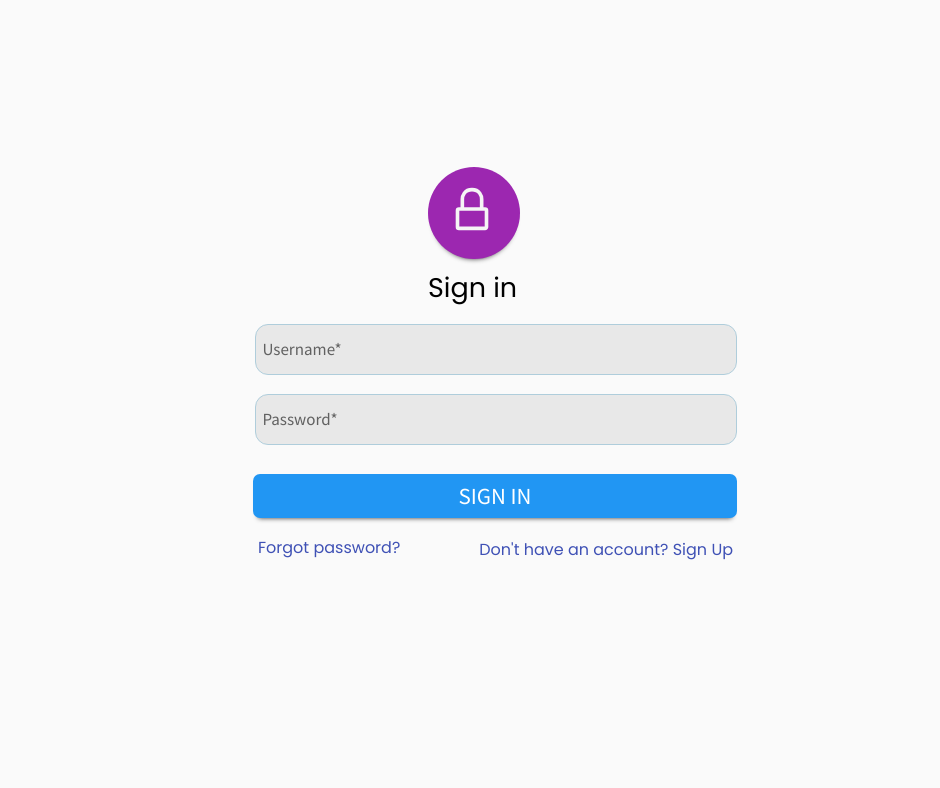
\includegraphics[width=1\linewidth]{fig/signin.png}
    \caption{Mockup de la Interfaz de Inicio de Sesión}
    \label{fig:signin}
\end{figure}

Como se evidencia en esta interfáz, el requisito de inicio de sesión solicita la introducción de un usuario y contraseña para acceder al sistema. Además, se ha incorporado la opción de recuperar la contraseña en caso de olvido, así como la capacidad de crear una nueva sesión para los usuarios que aún no cuentan con una cuenta registrada.


\subsection{Información de la Consulta}

Un requisito fundamental del sistema es la capacidad de visualizar la información detallada de cada consulta. Esta sección abarca diversos aspectos esenciales, incluyendo datos específicos de la consulta, una sección dedicada a comentarios, y una interfaz de calendario para gestionar fechas clave.

La Figura \ref{fig:info-consult-gui} presenta un mockup que ilustra la propuesta visual para la interfaz de información de consulta.

\begin{figure}[H]
\centering
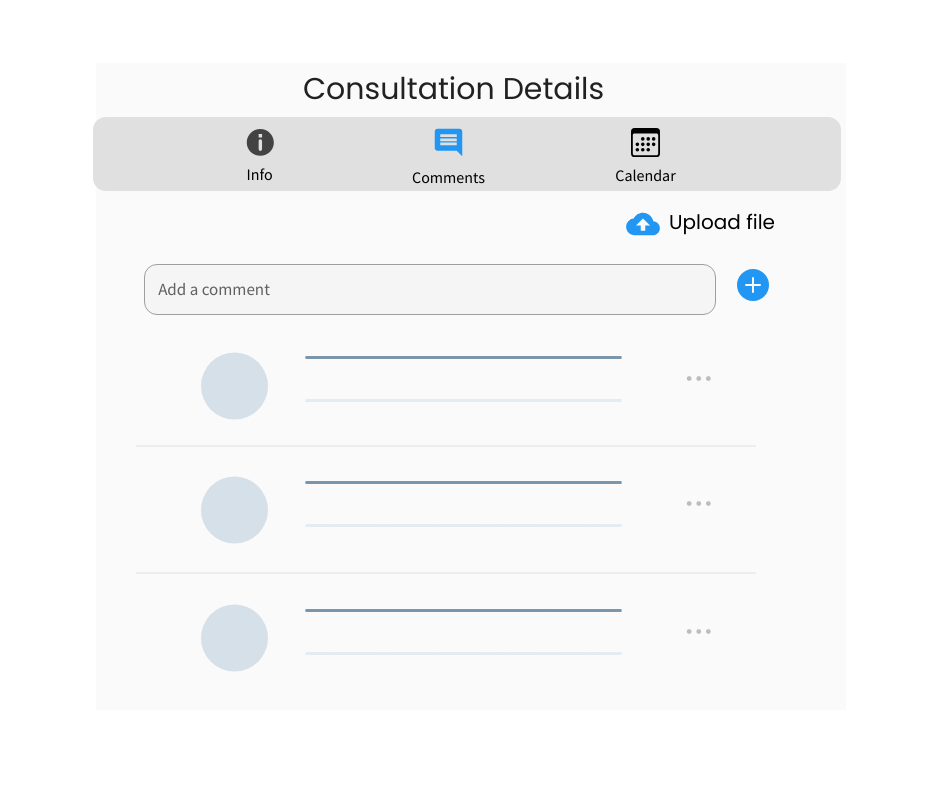
\includegraphics[width=1\linewidth]{fig/comment-gui.png}
\caption{Mockup de la Interfaz de Información de Consulta}
\label{fig:info-consult-gui}
\end{figure}

Esta interfaz permite interactuar a través de la sección de comentarios, permitiendo a los usuarios intercambiar información relevante, registrar datos y adjuntar archivos. Por otro lado, el calendario facilita la organización y seguimiento de eventos asociados a la consulta.

\subsection{Tablas de Control}

Se han requerido tablas para la visualización integral de todos los registros de consultas y clientes. En este contexto, se presenta un ejemplo con la tabla específica de consultas en la Figura \ref{fig:table-consult-gui}.

\begin{figure}[H]
\centering
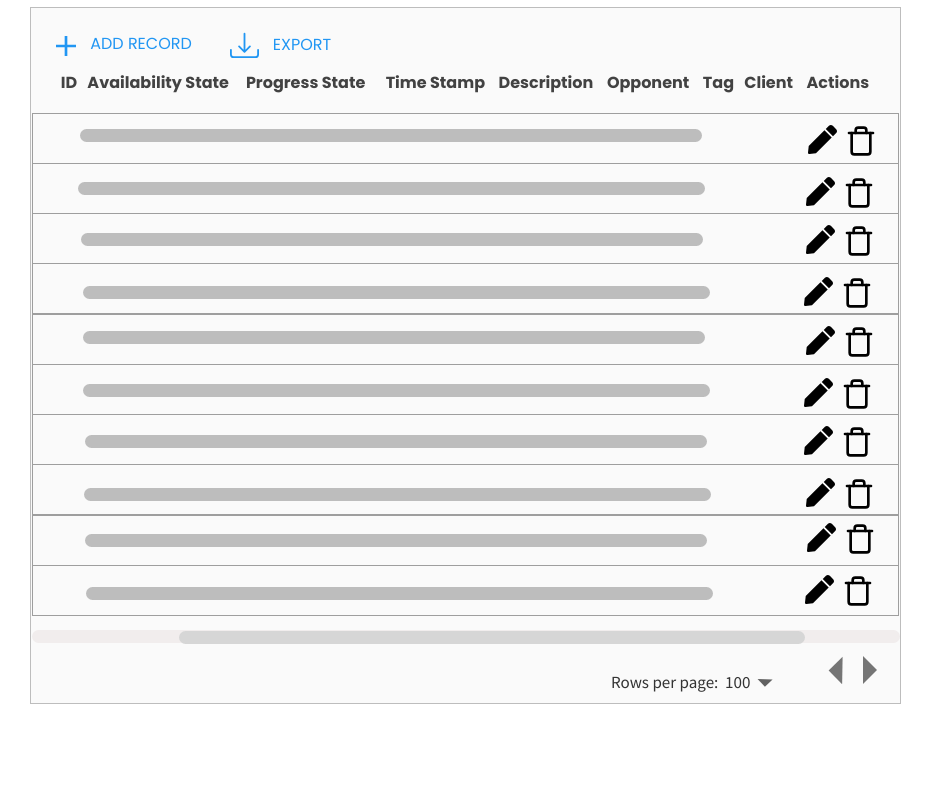
\includegraphics[width=1\linewidth]{fig/table-comment-gui.png}
\caption{Mockup de la Interfaz para las Tablas de Consultas}
\label{fig:table-consult-gui}
\end{figure}



\section{Requerimientos Funcionales}
Según Somerville \cite{Somerville}, Los requerimientos funcionaless son ``Son enunciados acerca de servicios que el sistema
debe proveer, de cómo debería reaccionar el sistema a entradas particulares y de cómo debería comportarse el sistema en situaciones específicas. En algunos casos, los requerimientos funcionales también explican lo que no debe hacer el sistema''

En el marco de este proyecto, los requerimientos funcionales se agrupan según sus funcionalidades específicas:

\begin{table}[H]
\centering
\begin{tabular}{|l|l|}
\hline
\textbf{Referencia} & \textbf{Función} \\
\hline
\textbf{RF.1} & Sistema de solicitudes de asignación de casos \\
\hline
\textbf{RF.2} & Sistema de gestión de casos por comisión \\
\hline
\textbf{RF.3} & Sistema de registro de clientes y consultas \\
\hline
\textbf{RF.4} & Sistema de alertas y notificaciones \\
\hline
\textbf{RF.5} & Registro y Autenticación de Usuarios \\
\hline
\end{tabular}
\caption{Requerimientos Funcionales}
\label{tab:rf}
\end{table}



\subsection{Sistema de Solicitudes de Asignación de Casos}

\begin{table}[H]
    \centering
    \begin{tabular}{|c|p{10cm}|}
        \hline
        \textbf{Referencia} & \textbf{Función} \\
        \hline
        RF.1.1 & Un Tomador de Caso podrá revisar la información de una consulta. \\
        \hline
        RF.1.2 & Un Tomador de Caso podrá revisar la cantidad de casos con sus estados de actividad de una comisión. \\
        \hline
        RF.1.3 & Un Tomador de Caso podrá revisar el historial reciente de solicitudes de una comisión. \\
        \hline
        RF.1.4 & Un Tomador de Caso podrá enviar una solicitud de asignación de un caso a una comisión. \\
        \hline
        RF.1.5 & Un Tomador de Caso podrá deshacer una solicitud de asignación. \\
        \hline
        RF.1.6 & Un Tomador de Caso podrá revisar la totalidad de casos. \\
        \hline
        RF.1.7 & Un Tomador de Caso podrá revisar la totalidad de clientes. \\
        \hline
    \end{tabular}
    \caption{Requerimientos Funcionales para Tomadores de Caso}
    \label{tab:rf-tomadores-caso}
\end{table}



\subsection{Sistema de Gestión de Casos por Comisión}
\begin{table}[H]
    \centering
    \begin{tabular}{|c|p{10cm}|}
        \hline
        \textbf{Requerimiento} & \textbf{Función} \\
        \hline
        RF.2.1 & Un usuario de una comisión tendrá la capacidad de aceptar o rechazar una solicitud de asignación de un nuevo caso a su comisión. \\
        \hline
        RF.2.2 & Un usuario de una comisión podrá visualizar los casos asignados a la comisión, incluyendo su estado y detalles relevantes. \\
        \hline
        RF.2.3 & Un usuario de una comisión podrá realizar modificaciones en los casos asignados a la comisión, actualizando la información según sea necesario. \\
        \hline
        RF.2.4 & Un usuario de una comisión podrá comentar en los casos asignados a la comisión, proporcionando información adicional o aclaraciones con la posibilidad de adjuntar archivos. \\
        \hline
        RF.2.5 & Un usuario de una comisión tendrá la opción de agregar y quitar eventos en los casos asignados a la comisión, permitiendo un seguimiento detallado de las actividades relacionadas con cada caso. \\
        \hline
    \end{tabular}
    \caption{Requerimientos Funcionales del Sistema de Gestión de Casos por Comisión}
    \label{tab:rf-gestion-casos-comision}
\end{table}

\subsection{Sistema de Registro de Clientes y Consultas}

\begin{table}[H]
    \centering
    \begin{tabular}{|l|p{10cm}|}
        \hline
        \textbf{Requerimiento} & \textbf{Descripción} \\
        \hline
        RF.3.1 & Un Tomador de Caso o Super Usuario podrá almacenar los datos de un cliente en el sistema. \\
        \hline
        RF.3.2 & Un Tomador de Caso o Super Usuario podrá registrar los detalles de una consulta de un cliente en el sistema. \\
        \hline
        RF.3.3 & El sistema permitirá cargar clientes mediante la integración con Google Forms, agilizando el ingreso de datos al sistema. \\
        \hline
        RF.3.4 & El sistema permitirá cargar consultas mediante la integración con Google Forms, facilitando el registro eficiente de información relacionada con las consultas de los clientes. \\
        \hline
    \end{tabular}
    \caption{Requerimientos del Sistema de Registro de Clientes y Consultas}
    \label{tab:registro-clientes-consultas}
\end{table}


\subsection{Sistema de Notificaciones y Alertas}

\begin{table}[H]
    \centering
    \begin{tabular}{|l|p{10cm}|}
        \hline
        \textbf{Requerimiento} & \textbf{Descripción} \\
        \hline
        RF.4.1 & El sistema podrá enviar correos electrónicos para notificar a los Tomadores de Caso cuando una solicitud es aceptada o rechazada. \\
        \hline
        RF.4.2 & El sistema podrá enviar correos electrónicos a los usuarios de una comisión al llegar una nueva solicitud de asignación de caso. \\
        \hline
        RF.4.3 & El sistema enviará alertas en tiempo real a los Tomadores de Caso cuando una solicitud es aceptada o rechazada. \\
        \hline
        RF.4.4 & El sistema enviará alertas a los usuarios de una comisión al llegar una solicitud de asignación de caso. \\
        \hline
        RF.4.5 & El sistema enviará alertas cuando ingresa un nuevo cliente o consulta a través de Google Forms, manteniendo a los usuarios informados sobre las actualizaciones en el sistema. \\
        \hline
    \end{tabular}
    \caption{Requerimientos del Sistema de Notificaciones y Alertas.}
    \label{tab:notificaciones-alertas}
\end{table}

\subsection{Registro y Autenticación de Usuarios}

\begin{table}[H]
    \centering
    \begin{tabular}{|l|p{10cm}|}
        \hline
        \textbf{Requerimiento} & \textbf{Descripción} \\
        \hline
        RF.5.1 & Un usuario podrá acceder a la plataforma mediante un nombre de usuario y contraseña. \\
        \hline
        RF.5.2 & Un usuario podrá registrarse en la plataforma a través de un proceso de autenticación vía correo electrónico. El acceso a la plataforma estará condicionado a la aceptación por parte de un usuario administrador. \\
        \hline
        RF.5.3 & Un usuario tendrá la capacidad de cambiar su contraseña en caso de olvidarla. \\
        \hline
        RF.5.4 & La plataforma permitirá a los usuarios visualizar únicamente las páginas para las cuales tengan permisos. \\
        \hline
    \end{tabular}
    \caption{Requerimientos de Registro y Autenticación de Usuarios.}
    \label{tab:registro-autenticacion}
\end{table}

\section{Requerimientos No Funcionales}
Según Somerville \cite{Somerville}, los requerimientos no funcionales son ``Son limitaciones sobre servicios o funciones que
ofrece el sistema. Incluyen restricciones tanto de temporización y del proceso de
desarrollo, como impuestas por los estándares. Los requerimientos no funcionales
se suelen aplicar al sistema como un todo, más que a características o a servicios
individuales del sistema.''

\begin{table}[H]
\centering
\begin{tabular}{|l|l|}
\hline
\textbf{Referencia} & \textbf{Función} \\
\hline
\textbf{RNF.1} & Requerimientos del producto \\
\hline
\textbf{RNF.2} & Requerimientos de la organización \\
\hline
\textbf{RNF.3} & Requerimientos externos \\
\hline
\end{tabular}
\caption{Requerimientos No Funcionales}
\label{tab:rnf}
\end{table}

\subsection{Requerimientos del producto}

\begin{table}[H]
    \centering
    \begin{tabular}{|l|p{10cm}|}
        \hline
        \textbf{Requerimiento} & \textbf{Descripción} \\
        \hline
        RNF.1.1 & El sistema se podrá acceder a través de la web desde una computadora con acceso a internet. \\
        \hline
        RNF.1.2 & La interfaz de usuario deberá ser intuitiva y fácil de usar, siguiendo los principios de diseño de experiencia de usuario (UX). \\
        \hline
        RNF.1.3 & El sistema deberá ser capaz de manejar simultáneamente por 5 a 10 usuarios sin degradación del rendimiento. \\
        \hline
        RNF.1.4 & El acceso a ciertas funcionalidades estará restringido a usuarios autorizados mediante roles y permisos. \\
        \hline
    \end{tabular}
    \caption{Requerimientos del Producto.}
    \label{tab:rnf-producto}
\end{table}

\subsection{Requerimientos de la organización}

\begin{table}[H]
    \centering
    \begin{tabular}{|l|p{10cm}|}
        \hline
        \textbf{Requerimiento} & \textbf{Descripción} \\
        \hline
        RNF.2.1 & La PC del usuario deberá tener un mínimo de 4GB de RAM y tarjeta de red para la conexión a internet. \\
        \hline
        RNF.2.2 & La plataforma será compatible con versiones estables de Chrome \(>=\) 120.0.6099.* y accesible a través de pantallas medianas a grandes. \\
        \hline
        RNF.2.3 & El código fuente deberá seguir buenas prácticas de desarrollo y ser fácilmente mantenible. \\
        \hline
    \end{tabular}
    \caption{Requerimientos de la Organización.}
    \label{tab:rnf-organizacion}
\end{table}

\subsection{Requerimientos externos}

\begin{table}[H]
    \centering
    \begin{tabular}{|l|p{10cm}|}
        \hline
        \textbf{Requerimiento} & \textbf{Descripción} \\
        \hline
        RNF.3.1 & Un usuario deberá aceptar los términos y condiciones para el registro a la plataforma. \\
        \hline
        RNF.3.2 & El sistema debe aplicar una política de complejidad de contraseñas que incluya la longitud mínima, uso de mayúsculas, minúsculas, números y caracteres especiales. \\
        \hline
        RNF.3.3 & Se debe implementar una protección efectiva contra ataques de fuerza bruta en las interfaces administrativas, incluyendo mecanismos de bloqueo temporal de cuentas. \\
        \hline
        RNF.3.4 & La integración con Google Forms y la API debe utilizar tokens de seguridad para autenticar y autorizar las solicitudes, manteniendo un flujo seguro de información. \\
        \hline
        RNF.3.5 & La plataforma deberá implementar medidas de seguridad contra ataques CSRF Token. \\
        \hline
        RNF.3.6 & La comunicación entre el servidor y los usuarios debe estar cifrada mediante un certificado SSL proporcionado por Let's Encrypt y configurado en el servidor Nginx. \\
        \hline
    \end{tabular}
    \caption{Requerimientos Externos.}
    \label{tab:rnf-externos}
\end{table}


\section{Definición de Roles y Responsabilidades}

\begin{table}[H]
    \centering
    \begin{tabular}{|p{3cm}|p{12cm}|}
        \hline
        \textbf{Tomador de Caso} & Este usuario tiene acceso al tablero de la consultoría y al panel de control. Su responsabilidad principal es agregar clientes y consultas de forma manual, además de asignar las consultas a una comisión específica. Los Tomadores de Caso pueden visualizar el estado de cada comisión, revisando la cantidad de casos activos y las últimas solicitudes enviadas.\\
        \hline
        \textbf{Integrante de Comisión (Profesor)} & Este rol se asigna a los integrantes de una comisión con acceso al tablero. Sus responsabilidades incluyen aceptar o rechazar solicitudes de asignación de casos o consultas. Además, se encargan de gestionar el seguimiento y progreso de cada caso asignado a su comisión.\\
        \hline
        \textbf{Jefe de Patrocinio (Administrador)} & También conocido como administrador, este usuario tiene privilegios que le otorgan acceso total a la plataforma. Sus responsabilidades principales incluyen la gestión de usuarios, permisos y roles, asegurando el correcto funcionamiento y la seguridad de la plataforma.\\
        \hline
        \textbf{Cliente (por Google Forms)} & Consultante que busca patrocinio gratuito. Este actor no tiene acceso directo a la plataforma y no ingresa a ella. Su interacción se limita a completar formularios de registro de cliente y consulta, los cuales se cargan automáticamente en la plataforma desde \textbf{Google Forms}.\\
        \hline

    \end{tabular}
    \caption{Roles y Responsabilidades de los Actores en la Plataforma}
    \label{tab:roles-responsabilidades}
\end{table}


\section{Diagrama de Caso de Uso del Sistema}
A continuación, se presentan los diagramas de caso de uso \ref{fig:caso-de-uso} para identificar a los actores implicados en una interacción. Si bien en este caso no se relacionan los casos de uso a alto nivel con diferentes actores, no significa que no exista una relación. Por otro lado, debe entenderse que Google Forms también cumple un rol e interactúa con el sistema principal Case Management System.

\begin{figure}[H]
\centering
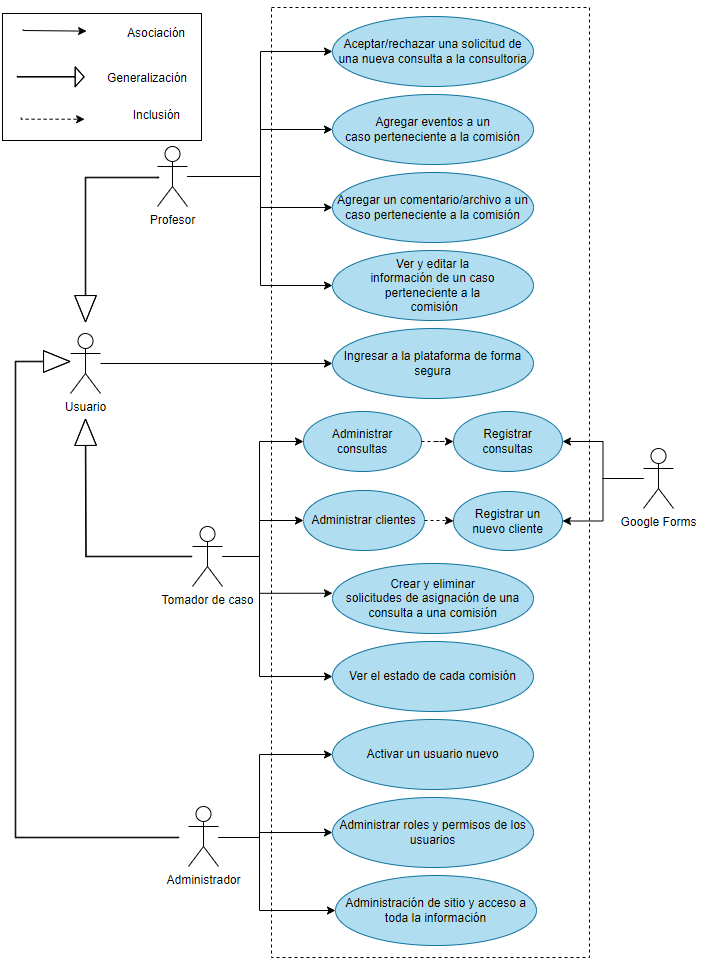
\includegraphics[width=1\linewidth]{fig/caso-de-uso.png}
\caption{Diagrama Caso de Uso}
\label{fig:caso-de-uso}
\end{figure}

\begin{itemize}
\item \textbf{CU.1}: Aceptar/rechazar una solicitud de una nueva consulta a la consultoría.
\item \textbf{CU.2}: Agregar eventos a un caso perteneciente a la comisión.
\item \textbf{CU.3}: Agregar un comentario/archivo a un caso perteneciente a la comisión.
\item \textbf{CU.4}: Ingresar a la plataforma de forma segura.
\item \textbf{CU.5}: Administrar consultas.
\item \textbf{CU.6}: Administrar clientes.
\item \textbf{CU.7}: Crear y eliminar solicitudes de asignación de una consulta a una comisión.
\item \textbf{CU.8}: Ver el estado de cada comisión.
\item \textbf{CU.9}: Activar a un usuario nuevo.
\item \textbf{CU.10}: Administrar roles y permisos de los usuarios.
\item \textbf{CU.11}: Administración de sitio y acceso a toda la información.
\end{itemize}


\section{Diagrama de Secuencia Nominal Simplificado}
A continuación, se incluye un diagrama de secuencia \ref{fig:secuencia-nominal} simplificado de alto nivel que representa una secuencia nominal para agregar comprensión a la funcionalidad de cada actor y su interacción con otros actores.

\begin{figure}[H]
\centering
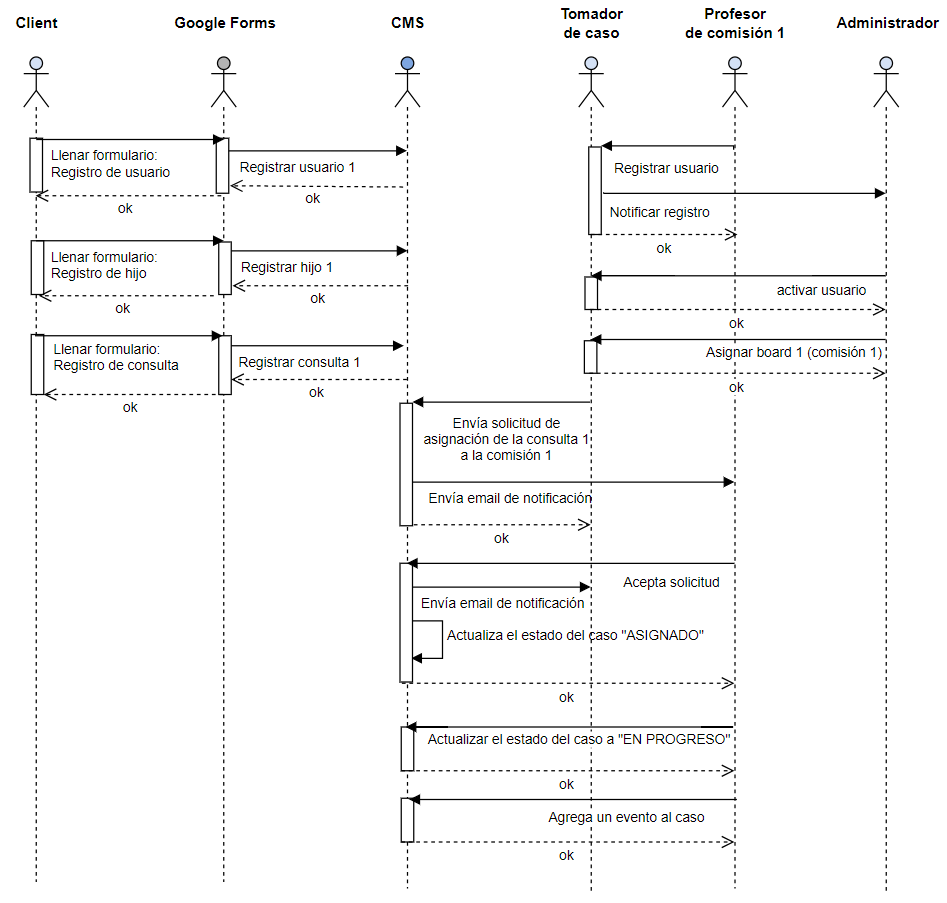
\includegraphics[width=1\linewidth]{fig/secuencia-basica.png}
\caption{Diagrama de Secuencia Simplificado}
\label{fig:secuencia-nominal}
\end{figure}

En este diagrama, participan varios actores, incluyendo un cliente con un solo hijo, el sistema externo Google Forms, el sistema Case Management System, el usuario tomador de caso, el profesor de la comisión número uno y el jefe de patrocinio o administrador.

Además, se detallan dos eventos en paralelo: el registro de un usuario en la plataforma y el registro de un cliente con una nueva consulta.

\section{Matriz de Trazabilidad}
La siguiente matriz de trazabilidad relaciona cada uno de los requerimientos con los casos de uso.

\begin{table}[H]
    \centering
    \small
    \begin{tabular}{|c|@{}c|@{}c|@{}c|@{}c|@{}c|@{}c|@{}c|@{}c|@{}c|@{}c|@{}c|}
    \hline
               & \textbf{CU1} & \textbf{CU2} & \textbf{CU3} & \textbf{CU4} & \textbf{CU5} & \textbf{CU6} & \textbf{CU7} & \textbf{CU8} & \textbf{CU9} & \textbf{CU10} & \textbf{CU11}\\
    \hline
    \hline
        \textbf{RF.1.1} &  &  & & &  & $\bullet$&  &  &  & & \\
        \hline
        \textbf{RF.1.2} &  &  & & &  &  &  &  & $\bullet$ & & \\
        \hline
        \textbf{RF.1.3} &  &  & &  &  &  &  &  & $\bullet$ & & \\
        \hline
        \textbf{RF.1.4} &  &  & &  &  &  &  & $\bullet$ &  & & \\
        \hline
        \textbf{RF.1.5} &  &  & &  &  &  &  & $\bullet$ &  & & \\
        \hline
        \textbf{RF.1.6} &  &  & &  &  & $\bullet$ &  &  &  & & \\
        \hline
        \textbf{RF.1.7} &  &  & &  &  &  &  $\bullet$ &  &  & & \\
        \hline
        \textbf{RF.2.1} & $\bullet$ &  &  & &  &  &  &  &  & & \\
        \hline
        \textbf{RF.2.2} &  &  &  & & $\bullet$ &  &  &  &  & & \\
        \hline
        \textbf{RF.2.3} &  &  & & & $\bullet$ &  &  &  &  & & \\
        \hline
        \textbf{RF.2.4} &  &  & $\bullet$ & & &  &  &  &  & & \\
        \hline
        \textbf{RF.2.5} &  & $\bullet$ &  & & &  &  &  &  & & \\
        \hline
        \textbf{RF.3.1} &  &  &  & &  &  & $\bullet$ &  &  & & $\bullet$ \\
        \hline
        \textbf{RF.3.2} &  &  &  & & & $\bullet$ &  &  &  & & $\bullet$ \\
        \hline
        \textbf{RF.3.3} &  &  &  & & &  & $\bullet$ &  &  & & \\
        \hline
        \textbf{RF.3.4} &  &  &  & & & $\bullet$ &  &  &  & & \\
        \hline
        \textbf{RF.4.1} & $\bullet$ & & &  &  &  &  &  &  & & \\
        \hline
        \textbf{RF.4.2} &  &  & & &  &  &  & $\bullet$ &  & & \\
        \hline
        \textbf{RF.4.3} & $\bullet$ &  & &  &  &  &  &  &  & & \\
        \hline
        \textbf{RF.4.4} &  &  &  & &  &  &  & $\bullet$ &  & & \\
        \hline
        \textbf{RF.4.5} &  &  &  & & &  & $\bullet$ &  &  & & \\
        \hline
        \textbf{RF.5.1} &  &  &  & $\bullet$ & &  &  &  &  & & \\
        \hline
        \textbf{RF.5.2} &  &  &  & $\bullet$ & &  &  &  & & & \\
        \hline
        \textbf{RF.5.3} &  &  &  & $\bullet$ &  &  &  &  &  & & \\
        \hline
        \textbf{RF.5.4} &  &  &  &&  &  &  &  &  & $\bullet$ & \\
    \hline
        \textbf{RNF.1.1} &  &  & & &  &  &  &  &  & & \\
        \hline
        \textbf{RNF.1.2} &  &  & & &  &  &  &  &  & & \\
        \hline
        \textbf{RNF.1.3} &  &  & & &  &  &  &  &  & & \\
        \hline
        \textbf{RNF.1.4} &  &  & & &  &  &  &  &  & $\bullet$ & \\
        \hline
        \textbf{RNF.2.1} &  &  & & &  &  &  &  &  & & \\
        \hline
        \textbf{RNF.2.2} &  &  & & &  &  &  &  &  & & \\
        \hline
        \textbf{RNF.2.3} &  &  & & &  &  &  &  &  & & \\
        \hline
        \textbf{RNF.3.1} &  &  & & &  &  &  &  &  & & \\
        \hline
        \textbf{RNF.3.2} &  &  &&  &  &  &  &  &  & & \\
        \hline
        \textbf{RNF.3.3} &  &  & & &  &  &  &  &  & & \\
        \hline
        \textbf{RNF.3.4} &  &  & & &  &  &  &  &  & & \\
        \hline
        \textbf{RNF.3.5} &  &  & & &  &  &  &  &  & & \\
        \hline
        \textbf{RNF.3.6} &  &  &  & &  &  &  &  &  & & \\
    \hline
    \end{tabular}
    \caption{Matriz de Trazabilidad}
    \label{tab:matriz-trazabilidad}
\end{table}


    \chapter{Arquitectura y Diseño}\label{cap:arquitectura-diseño}

\section{Introducción}
En este capítulo, se presenta la arquitectura y el diseño del sistema implementado. Se abordan los principios y decisiones arquitectónicas que guiaron el desarrollo del sistema, así como los modelos y diagramas que ilustran la estructura y comportamiento del mismo.


\section{Modelado del sistema}
Según Somerville, el modelado de sistemas es un proceso para desarrollar modelos abstractos que representan diferentes perspectivas de un sistema. Estos modelos, que a menudo utilizan notaciones gráficas basadas en el Lenguaje de Modelado Unificado (UML), desempeñan un papel importante en la ingeniería de requerimientos y el diseño del sistema \cite{Somerville}. 
En esta sección se modelan las perspectivas de contexto o entorno, de interacción, estructural y de comportamiento para proporcionar una comprensión integral del sistema.


\subsection{Modelo de Contexto}

En la figura \ref{fig:c4-01}, se identifican dos sistemas externos que interactúan con la plataforma:

\begin{itemize}
    \item \textbf{Google Forms:} Utilizado para el envío de formularios, facilitando el ingreso de consultantes y consultas.
    \item \textbf{Email:} El sistema de correo electrónico, como Gmail, se conecta a la plataforma para el envío de notificaciones y el registro de nuevos usuarios.
\end{itemize}

Por otro lado, se encuentran los distintos tipos de usuarios que acceden a la plataforma:

\begin{itemize}
    \item \textbf{Tomadores de Caso:} Administran los casos, asignándolos a diferentes comisiones.
    \item \textbf{Jefes de Patrocinio:} Ingresan a la página de administración para gestionar permisos de usuarios, aprobar nuevos ingresos, visualizar información general y editar configuraciones.
    \item \textbf{Integrantes de Comisión:} Profesores, jefes de trabajo práctico y/o jefe de comisión que acceden al tablero de su comisión para gestionar los casos.
    \item \textbf{Alumnos:} Los alumnos no acceden directamente a la plataforma; en su lugar, envían información al profesor, quien gestiona los casos.
    \item \textbf{Clientes:} No ingresan a la plataforma; en su lugar, completan formularios que se envían al sistema.
\end{itemize}

\begin{figure}[H]
    \centering
    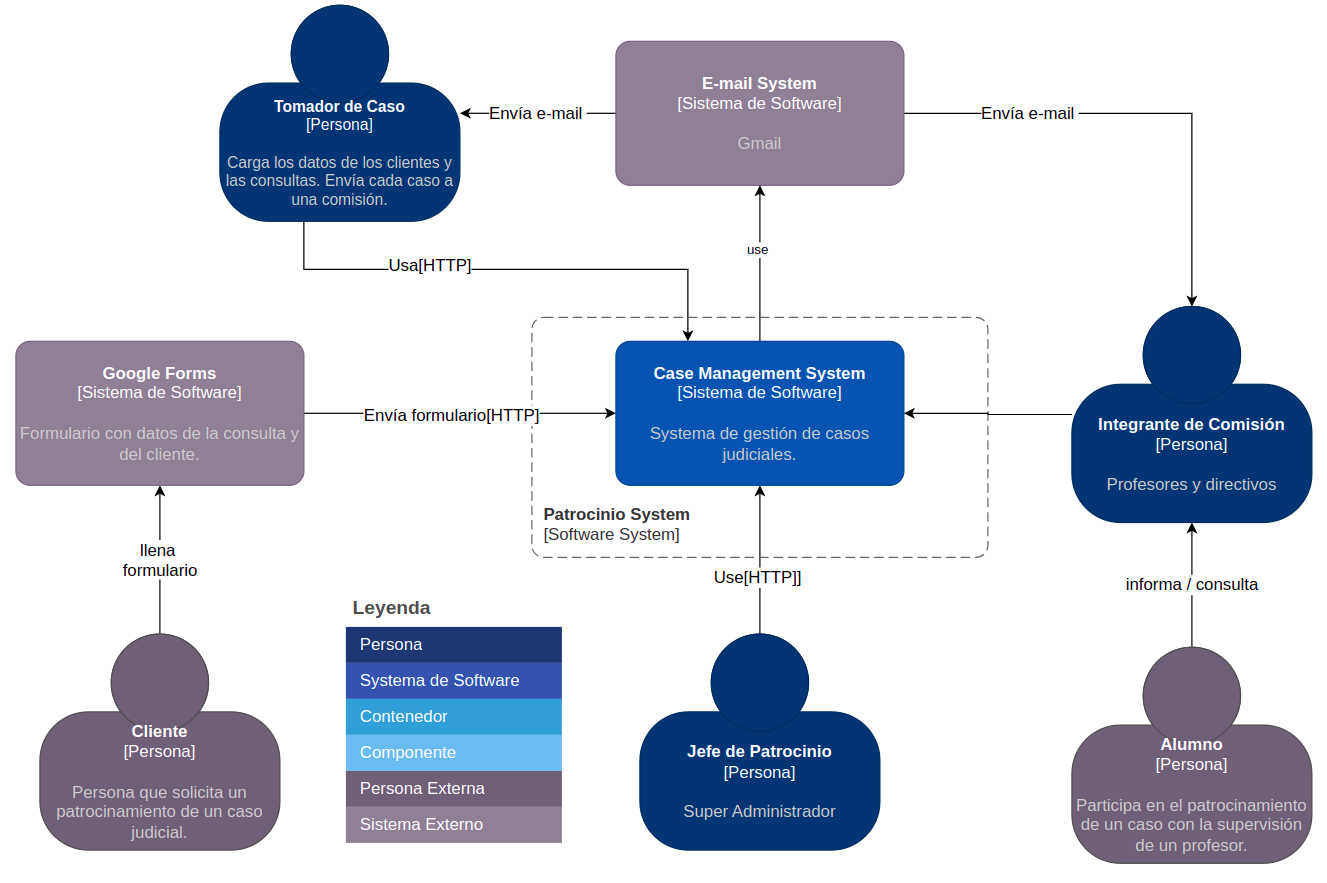
\includegraphics[width=1.1\linewidth]{fig/c4-1.png}
    \caption{Diagrama de Contexto C4}
    \label{fig:c4-01}
\end{figure}



\subsection{Modelo de Contenedores}
Si profundizamos, observamos cómo está conformado el sistema a nivel de contenedores.

Un ``contenedor'' no se limita a la noción convencional de un contenedor Docker; más bien, representa una aplicación, un almacén de datos o cualquier entidad desplegable de manera independiente, abarcando desde aplicaciones web hasta sistemas de archivos.

\begin{figure}[h]
\centering
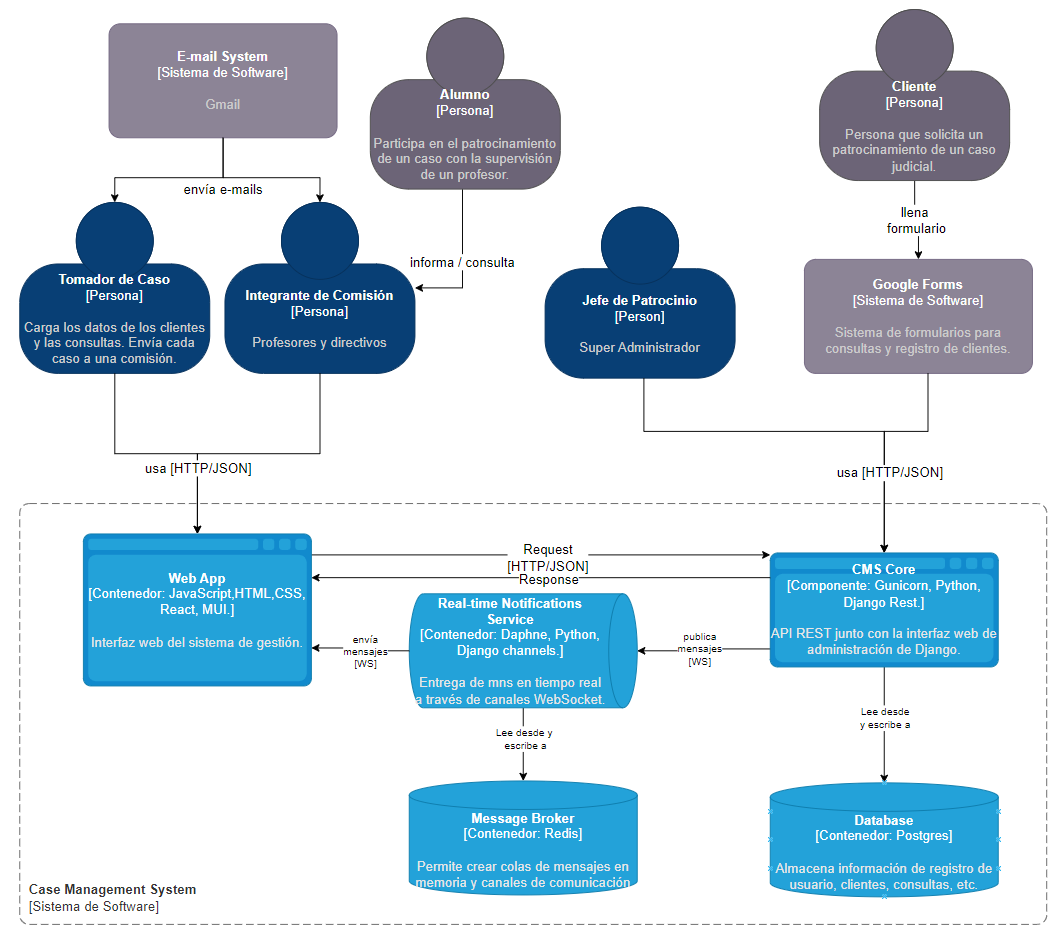
\includegraphics[width=1\linewidth]{fig/c4-2.png}
\caption{Diagrama de Contenedores C4}
\label{fig:c4-02}
\end{figure}

\begin{itemize}
\item \textbf{Web App:} Proporciona una interfaz web para el sistema de gestión de casos destinado a las comisiones y consultoría.
\item \textbf{Real-time Notifications Service:} Utiliza Django ASGI con WebSockets para la entrega de notificaciones en tiempo real.
\item \textbf{Redis:} Actúa como un almacén en memoria y se utiliza para gestionar las comunicaciones en tiempo real a través de Pub/Sub.
\item \textbf{CMS Core:} Proporciona una API REST en Django con la lógica de negocio. También ofrece la interfaz de administración de Django.
\end{itemize}




\subsection{Modelo de Componentes}
A continuación, se desglosan algunos contenedores para identificar los componentes estructurales principales y sus interacciones mediante los siguientes diagramas.

En el diagrama del contenedor CMS Core, se presentan los componentes clave y sus relaciones internas.
\begin{figure}[H]
\centering
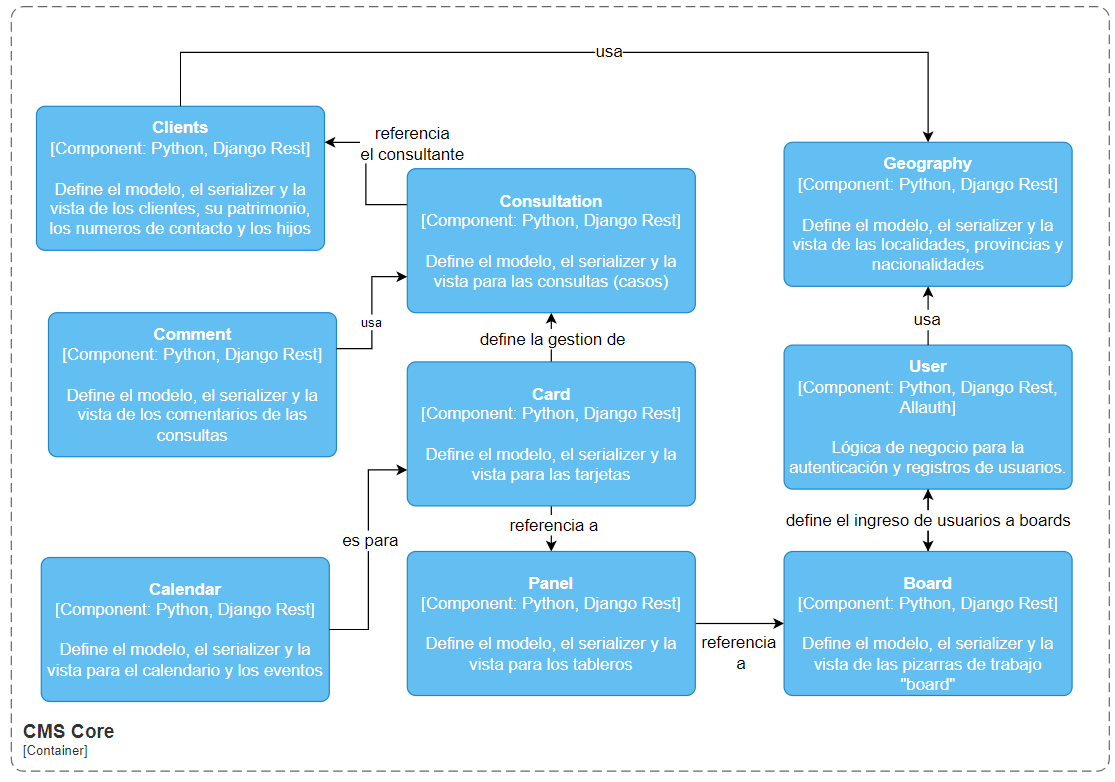
\includegraphics[width=1\linewidth]{fig/container-cms-core.png}
\caption{Diagrama de Componentes C4 del Contenedor CMS Core}
\label{fig:c4-03-cmscore}
\end{figure}
Este diagrama ilustra cómo el contenedor CMS Core incorpora cada componente de la API REST de manera modular, junto con la interfaz de usuario proporcionada por Django para la administración.

Asimismo, a continuación, se presenta el diagrama de componentes del contenedor Web App con sus principales elementos.
\begin{figure}[H]
\centering
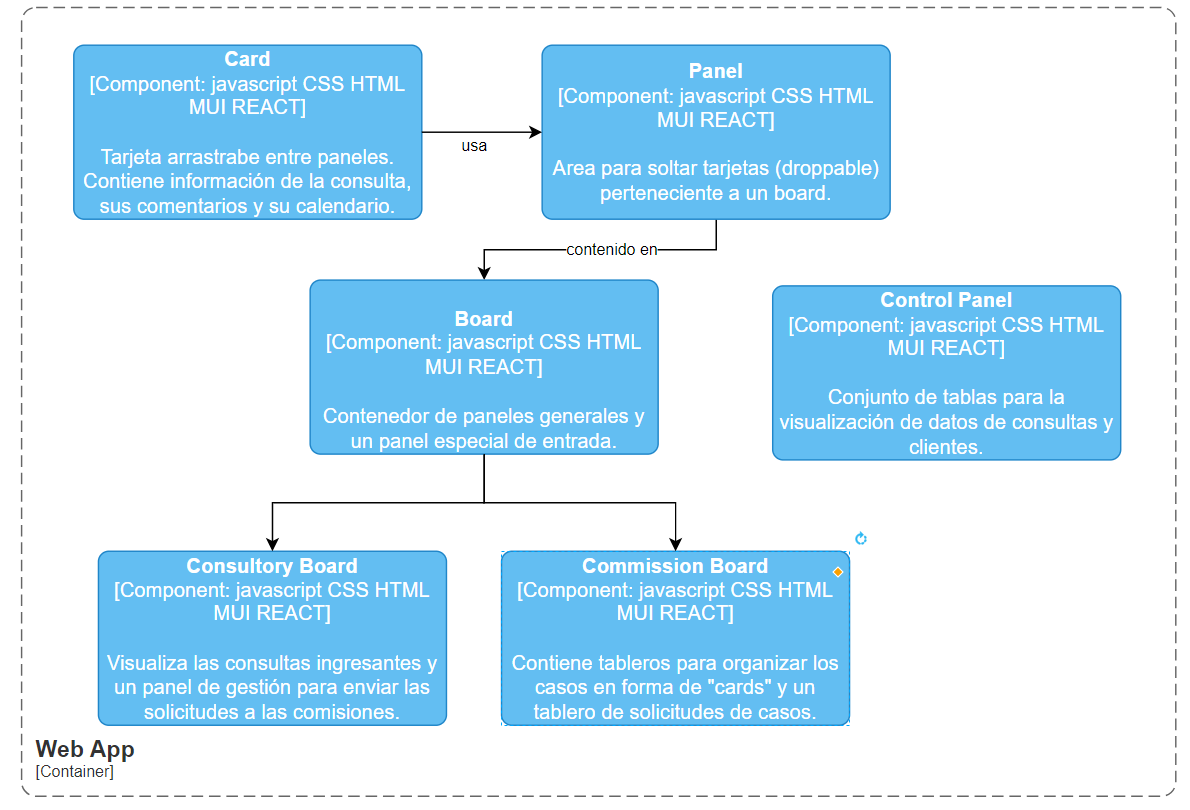
\includegraphics[width=1\linewidth]{fig/container-web-app.png}
\caption{Diagrama de Componentes C4 del Contenedor Web App}
\label{fig:c4-03-webapp}
\end{figure}
En este diagrama, se detalla la estructura del tablero (Board), que contiene paneles y, a su vez, cada panel alberga tarjetas (Cards). Además, se distinguen dos tipos de tableros: ``Consultancy'' para la consultoría y ``Commission Board'' para la pizarra de trabajo de cada comisión. Por separado, se encuentra el ``Control Panel'', que consta de dos tablas para consultas y consultantes.


\section{Arquitectura}
La implementación del software seguirá el patrón de arquitectura cliente-servidor. Esta elección se fundamenta en la necesidad de alojar la aplicación web en el servidor de aplicaciones, permitiendo a los usuarios acceder a ella desde cualquier dispositivo con conexión a internet. Se optará por la arquitectura REST para la comunicación cliente-servidor. Además, para el sistema de notificaciones, se aplicará el patrón de arquitectura Mediador (Broker Pattern), haciendo uso del diseño de publicador-suscriptor.

\section{Desarrollo Modular de la Arquitectura REST en DRF}

Cuando se menciono que la API REST está estructurada de forma modular, se refiere a que cada componente se organiza como un módulo independiente (ver \ref{section:mt-api-ref}). Cada uno de estos módulos define las rutas, modelos y vistas necesarias para su funcionamiento.

\begin{figure}[H]
\centering
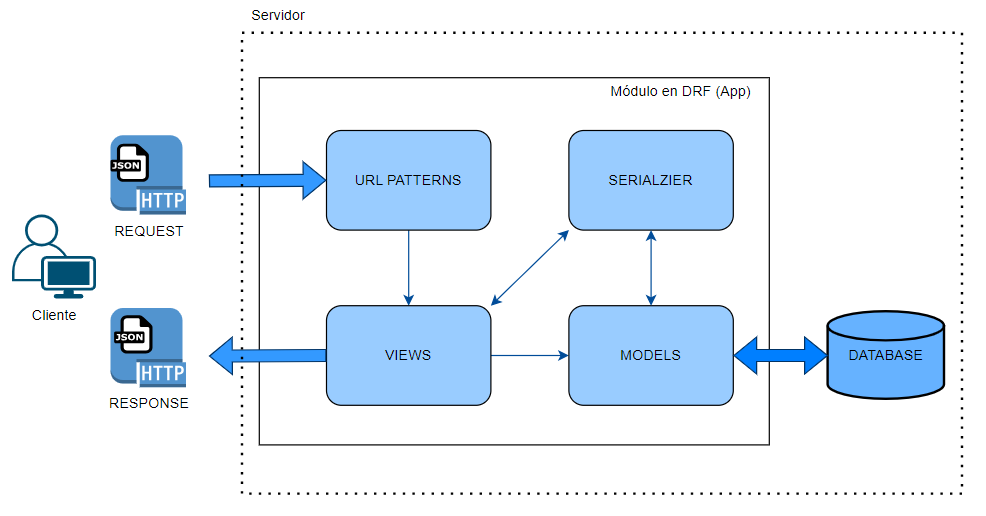
\includegraphics[width=1\linewidth]{fig/app-drf.png}
\caption{Diagrama de un Módulo en DRF}
\label{fig:app-drf}
\end{figure}

En la figura \ref{fig:app-drf}, los serializadores traducen la información de los modelos a un formato serializado (JSON) y viceversa. Las vistas establecen la lógica de negocio para manipular y procesar los datos antes de enviar una respuesta al cliente. Por otro lado, los modelos representan la estructura de los datos almacenados en la base de datos, proporcionando una abstracción entre la base de datos y las representaciones de datos expuestas a través de la API.

\section{Patrón de Arquitectura Mediador (Broker pattern)}
La implementación del patrón de arquitectura Mediador (Broker pattern) se logró mediante el uso de Django Channels y Redis como el componente Broker que coordina la comunicación entre los diversos elementos del sistema de notificaciones en tiempo real. En este contexto, el servidor publica sus servicios en el Broker, representados como ``canales'' (un canal para la consultoría y un canal por comisión).

Cuando un cliente requiere un servicio específico, se comunica con el Broker, el cual redirige al cliente hacia el servicio correspondiente según su registro.


\section{Implementación del Patrón de Diseño Pub/Sub sobre el Protocolo de comunicación Web Sockets}

En relación a la sección anterior, respecto al sistema de notificaciones en tiempor real, la implementación del patrón de diseño Publicador-Suscriptor (Pub/Sub \ref{sec:pub-sub}) sobre el protocolo de comunicación WebSockets se utiliza en la suscripción de un cliente a un canal y la publicación de mensajes del servidor a dicho canal.

\begin{figure}[H]
    \centering
    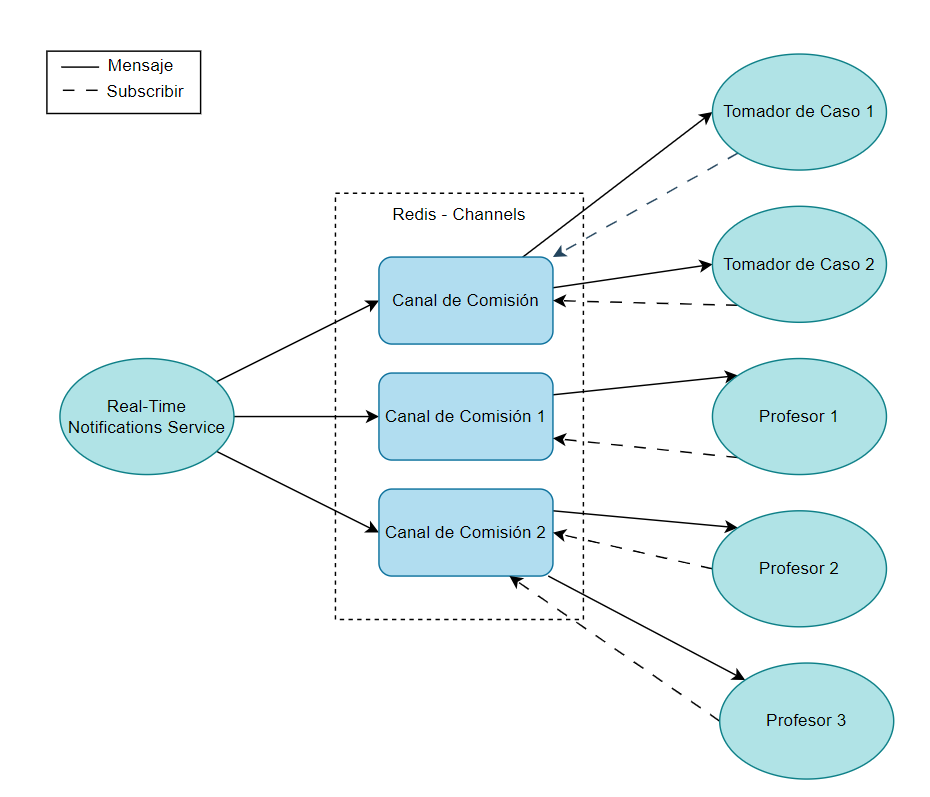
\includegraphics[width=0.9\linewidth]{fig/channels.png}
    \caption{Diagrama Implementación del Patrón Pub/Sub}
    \label{fig:channels-redis}
\end{figure}

Como se observa en la imagen, los canales representan una consultoría y un canal por cada comisión.


\section{Implementación Arrastrar y soltar}
Se utilizó el framework de JavaScript \textit{React-beautiful-dnd} para la creación de los ``Boards'', permitiendo al usuario tener una experiencia más intuitiva y rápida con la función de ``Arrastrar y soltar''. La similitud con Trello fue determinada en la etapa de gobernanza de datos y reingeniería de procesos, donde participó el equipo del Patrocinio Jurídico Gratuito de la Facultad de Derecho.

\begin{figure}[H] \centering 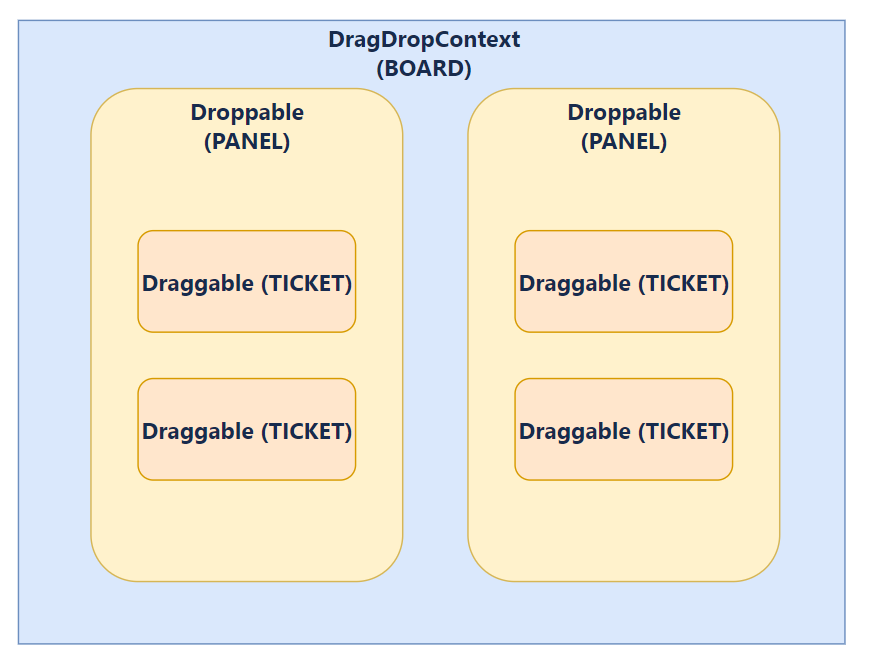
\includegraphics[width=1\linewidth]{fig/drag-drop.png} \caption{Estructura Drag and Drop} \label{fig:enter-label} \end{figure}

\begin{itemize}
    \item \textbf{DragDropContext}: Envuelve la parte de la aplicación para la que desea habilitar la función de arrastrar y soltar.
    \item \textbf{Droppable}: Esta es el área donde puede soltar y contiene.
    \item \textbf{Draggable}: Estos son los elementos que se pueden arrastrar.
\end{itemize}

A continuación, se presenta un diagrama de componentes que ilustra la estructura y relación de los elementos clave en la implementación del patrón de "Arrastrar y soltar" en el frontend.

\begin{figure}[H]
\centering
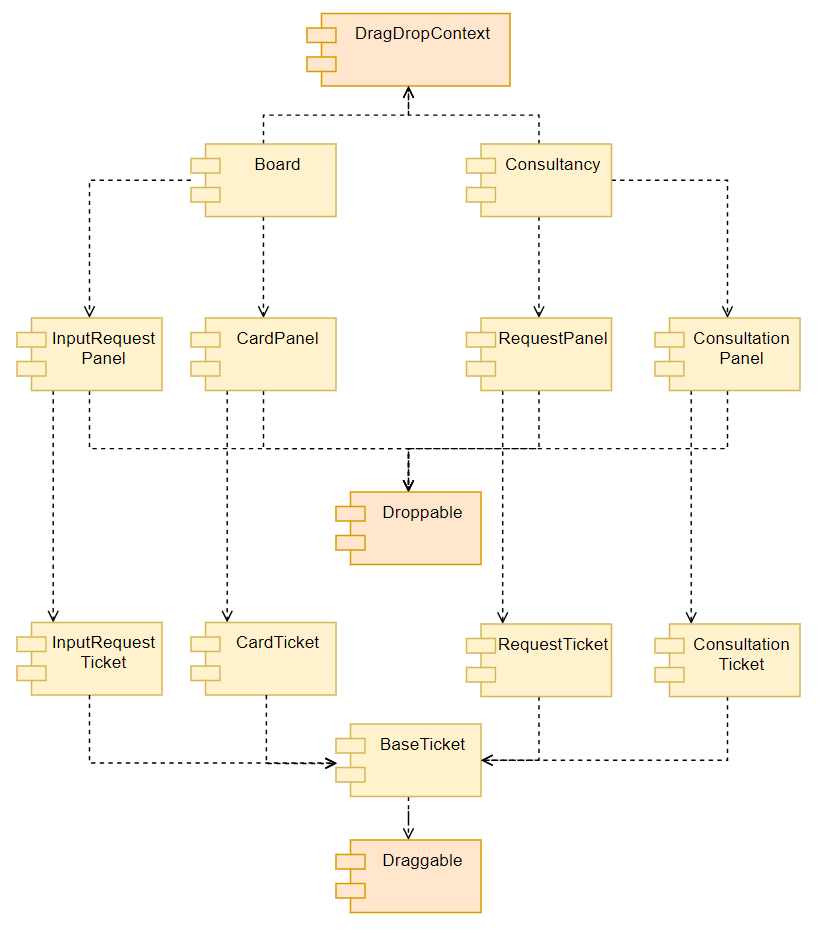
\includegraphics[width=0.90\linewidth]{fig/drag-drop-componentes.png}
\caption{Diagrama de Componentes Drag and Drop}
\label{fig:drag-drop-componentes}
\end{figure}

En la figura, se pueden observar diferentes tipos de pizarras, paneles y tickets. Cada pizarra representa un área de trabajo donde se organizan los paneles. Para cada pizarra, existen dos tipos de paneles: uno para la entrada de tickets y otro para la administración de los tickets propios de la consultoría o comisión, según corresponda. Los tickets se dividen en tres categorías: Solicitud, Consulta y Card. Los tickets de Solicitud se refieren a la solicitud de asignación de una consulta. Los tickets de Consulta son aquellos que se encuentran en la consultoría sin asignar, mientras que los tickets Card se refieren a los tickets asignados a una comisión.

    \input{sections/06_Implementación_Test}
    \chapter{Despliegue y Operación}\label{cap:sum}

\section{Introducción}
Este capítulo aborda el proceso integral de instalación y puesta en marcha del servicio, detallando el despliegue de la pila de contenedores en Swarm. Además, se proporciona una guía práctica sobre el uso efectivo de la misma.


\section{Instalación de la Plataforma}

Para iniciar el proceso de instalación, es necesario contar con el repositorio de deploy. Puede clonar el repositorio desde GitHub utilizando el siguiente comando:


%estilo de comando
\lstdefinestyle{consola} {
    numbers=none,
    xleftmargin=\parindent,
    xrightmargin=\parindent,
    aboveskip=3mm,
    belowskip=0.01mm,
    basicstyle=\small\bf\ttfamily,
    backgroundcolor=\color{black!08},
}


\begin{lstlisting}[style=consola]
$ git clone git@github.com:proyecto-patrocinio/proyecto-patrocinio.git
\end{lstlisting}

Una vez clonado el repositorio, es fundamental realizar la configuración previa de los archivos.
 A continuación, se proporciona una descripción detallada de los archivos de configuración del repositorio de deploy. 

\lstset{
  basicstyle=\ttfamily,
  breaklines=true,
  postbreak=\mbox{\textcolor{red}{$\hookrightarrow$}\space},
}

\begin{lstlisting}
.
|-- .env
|-- docker-compose.yml
|-- dotenv.sh
|-- README.md
|-- resources
|   |-- backend.env
|   |-- frontend.env
|   |-- nginx.conf
|   |-- postgres.env
|   |-- templates
|   |   |-- account
|   |   |   |-- email_confirmation_message.html
|   |   |   |-- email_confirmation_signup_message.html
|   |   |-- notifications
|   |   |   |-- new_request.html
|   |   |   |-- request_accepted.html
|   |   |   |-- request_rejected.html
|   |-- terms_and_policies.md
\end{lstlisting}




\subsection{Configuración de Templates}
\begin{enumerate}
    \item En la carpeta \texttt{\textbf{templates/account}}, se encuentran los siguientes templates:

\begin{itemize}
    \item \texttt{email\_confirmation\_signup\_message}: HTML enviado por email en la confirmación del registro de una cuenta.
    \item \texttt{email\_confirmation\_message}: HTML enviado por email cuando se solicita reenviar el email para el registro de usuario.
    \item \texttt{password\_reset\_key\_message}: HTML enviado por email cuando se solicitó cambiar contraseña olvidada.
\end{itemize}


 \item  En la carpeta \texttt{\textbf{templates/notifications}}, se encuentran los siguientes templates:

\begin{itemize}
    \item \texttt{new\_request}: HTML enviado por email para notificar al usuario cuando la comisión tiene una nueva solicitud de asignación de caso.
    \item \texttt{request\_accepted}: HTML enviado por email en la notificación al tomador de caso cuando una comisión aceptó una solicitud.
    \item \texttt{request\_rejected}: HTML enviado por email en la notificación al tomador de caso cuando una comisión rechazó una solicitud.
\end{itemize}


\end{enumerate}



\subsection{Configuración de Variables de Entorno en el Archivo \texttt{.env}}

En el archivo \texttt{.env}, se deben establecer las siguientes variables de entorno que serán reenderizadas por el archivo compose \textit{docker-compose.yml}. A continuación, se presenta una tabla con descripciones de cada variable:

\begin{table}[H]
    \centering
    \begin{tabular}{|l|p{7cm}|}
    \hline
    \textbf{Variable de Entorno} & \textbf{Descripción} \\
    \hline
    CMS\_BACKEND\_IMAGE & Nombre de la imagen de Docker para el backend. \\
    \hline
    CMS\_FRONTEND\_IMAGE & Nombre de la imagen de Docker para el frontend.\\
    \hline
    CMS\_PROXY\_PORT & Puerto del servidor proxy Nginx. \\
    \hline
    CMS\_NGINX\_CONFIG\_FILE & Ruta al archivo de configuración de NGINX. \\
    \hline
    CMS\_BACKEND\_ENV\_FILE & Ruta al archivo de variables de entorno para el backend. \\
    \hline
    CMS\_POSTGRES\_ENV\_FILE & Ruta al archivo de variables de entorno para PostgreSQL. \\
    \hline
    CMS\_FRONTEND\_ENV\_FILE & Ruta al archivo de variables de entorno para el frontend. \\
    \hline
    CMS\_TEMPLATES\_ACCOUNT\_PATH & Ruta al directorio de plantillas de ``account''. \\
    \hline
    CMS\_TEMPLATES\_NOTIFICATION\_PATH & Ruta al directorio de plantillas de ``notifications''.\\
    \hline
    CMS\_TERMS\_AND\_POLICIES\_FILE & Ruta al archivo de términos y políticas. \\
    \hline
    \end{tabular}
    \caption{Configuración de Variables de Entorno en el Archivo \texttt{.env}}
    \label{tab:env-file-variables}
\end{table}

Consulte el anexo para revisar las variables utilizadas: \ref{sec:anexo:configfile-env}.


\subsection{Configuración de Variables de Entorno en \texttt{backend.env}}

En el archivo \texttt{\textbf{backend.env}}, se deben configurar las siguientes variables de entorno. A continuación, se presenta una tabla con descripciones de cada variable:

\begin{table}[H]
    \centering
    \begin{tabular}{|l|p{7cm}|}
    \hline
    \textbf{Variable de Entorno} & \textbf{Descripción} \\
    \hline
    DEBUG & Modo de depuración (0 para desactivado, 1 para activado). \\
    \hline
    DJANGO\_ALLOWED\_HOSTS & Lista de hosts permitidos separados por espacios. \\
    \hline
    SQL\_ENGINE & Motor de base de datos para Django. Por ejemplo para postgres es `django.db.backends.postgresql'.\\
    \hline
    SQL\_DATABASE & Nombre de la base de datos. \\
    \hline
    SQL\_USER & Usuario de la base de datos. \\
    \hline
    SQL\_PASSWORD & Contraseña de la base de datos. \\
    \hline
    SQL\_HOST & Dirección del servidor de base de datos. \\
    \hline
    SQL\_PORT & Puerto del servidor de base de datos. \\
    \hline
    DATABASE & Tipo de base de datos. En este caso es `postgres'.\\
    \hline
    EMAIL\_HOST\_USER & Usuario del servidor de correo electrónico. \\
    \hline
    EMAIL\_HOST\_PASSWORD & Contraseña del servidor de correo electrónico. \\
    \hline
    CORS\_ALLOWED\_ORIGINS & Lista de orígenes permitidos para CORS. \\
    \hline
    HOSTNAME & Nombre del host de la aplicación. \\
    \hline
    CONSULTANCY\_BOARD\_NAME & Nombre de la comisión de consultoría. \\
    \hline
    DEFAULT\_HTTP\_PROTOCOL & Protocolo HTTP. \\
    \hline
    CSRF\_TRUSTED\_ORIGINS & Lista de orígenes confiables para CSRF. \\
    \hline
    LOG\_ROTATE\_DAYS & Días antes de rotar los archivos de log. \\
    \hline
    SECRET\_KEY & Clave secreta de Django. \\
    \hline
    DJANGO\_SUPERUSER\_USERNAME & Nombre de usuario del superusuario administrador para acceder a la web admin de Django. \\
    \hline
    DJANGO\_SUPERUSER\_PASSWORD & Contraseña del superusuario administrador del proyecto. \\
    \hline
    DJANGO\_SUPERUSER\_EMAIL & Correo electrónico del superusuario administrador. \\
    \hline
    \end{tabular}
    \caption{Configuración de Variables de Entorno en \texttt{backend.env}}
    \label{tab:env-variables}
\end{table}


Consulte el anexo para revisar las variables utilizadas: \ref{sec:anexo:configfile-backend-env}.


\subsection{Configuración de Variables de Entorno en \texttt{frontend.env}}

En el archivo \texttt{frontend.env}, se deben configurar las siguientes variables de entorno. A continuación, se presenta una tabla con descripciones de cada variable:

\begin{table}[H]
    \centering
    \begin{tabular}{|p{7cm}|p{7cm}|}
    \hline
    \textbf{Variable de Entorno} & \textbf{Descripción} \\
    \hline
    REACT\_APP\_URL\_BASE\_API
    \_REST\_PATROCINIO & URL base de la API REST de Patrocinio. Ejemplo https://\{\{dominio\}\}/api/. \\
    \hline
    REACT\_APP\_WS\_NOTIFICATION
    \_PATH\_PATROCINIO & Ruta del servidor asincrónico para notificaciones. Ejemplo wss://\{\{dominio\}\}/ws/notification/\\
        \hline
    \end{tabular}
    \caption{Configuración de Variables de Entorno en \texttt{frontend.env}}
    \label{tab:frontend-env-variables}
\end{table}
El resto de variables de entorno de este archivo no deben tocarse, son específicas para acceder a los endpoints del backend.

Consulte el anexo para revisar las variables utilizadas: \ref{sec:anexo:configfile-frontend-env}.



\subsection{Configuración de Variables de Entorno para la Base de Datos}

En el archivo \texttt{\textbf{backend.env}}, se deben configurar las siguientes variables de entorno relacionadas con la base de datos. A continuación, se presenta una tabla con descripciones de cada variable:

\begin{table}[H]
    \centering
    \begin{tabular}{|l|p{9cm}|}
    \hline
    \textbf{Variable de Entorno} & \textbf{Descripción} \\
    \hline
    POSTGRES\_DB & Nombre de la base de datos de Patrocinio en PostgreSQL. \\
    \hline
    POSTGRES\_USER & Usuario de la base de datos de Patrocinio en PostgreSQL. \\
    \hline
    PGDATA & Ruta del directorio de datos de PostgreSQL. \\
    \hline
    POSTGRES\_PASSWORD & Contraseña para el usuario de la base de datos de Patrocinio en PostgreSQL. \\
    \hline
    \end{tabular}
    \caption{Configuración de Variables de Entorno para la Base de Datos}
    \label{tab:database-env-variables}
\end{table}


Consulte el anexo para revisar las variables utilizadas: \ref{sec:anexo:configfile-portgres-env}.

\subsection{Archivo de Configuración de Nginx}

El archivo de configuración de Nginx puede obtener más información detallada en la sección correspondiente (\ref{subsec:nginx_explicacion}). Asegúrese de revisar esa sección para comprender y ajustar la configuración de Nginx según sea necesario para el correcto funcionamiento de la plataforma.

\subsection{Archivo \texttt{terms\_and\_policies}}

El archivo \texttt{terms\_and\_policies} debe configurarse según las políticas y términos que la plataforma desea establecer y que los usuarios deberán aceptar. Este archivo es crucial para definir las reglas y condiciones de uso de la plataforma.


\section{Despliegue de la Plataforma}

Para llevar a cabo el despliegue de la plataforma, se deben seguir los pasos detallados en el archivo README del repositorio de deploy.

Hasta la fecha actual, se dispone de un único nodo, que también actúa como nodo maestro, en el cual se ha implementado el despliegue mediante Docker Swarm. Este nodo maestro hospeda todos los servicios necesarios para la plataforma.

Inicialmente, el servidor ya contaba con un servidor Nginx en funcionamiento y un servicio de R Studio. Se procedió a integrar el servicio Case Management System en el servidor Nginx existente.

En la Figura \ref{fig:deploy-in-server} se presenta un diagrama que ilustra los servicios proporcionados por el servidor, destacando la composición del servicio Case Management System, definido a través de un Docker Stack.



Es importante tener en cuenta que si se decide agregar nodos adicionales al clúster de Docker Swarm, será necesario actualizar el controlador de volúmenes de Docker Swarm. Esto se realiza para permitir el intercambio de volúmenes entre los diferentes nodos del clúster.

\begin{figure}[H]
\centering
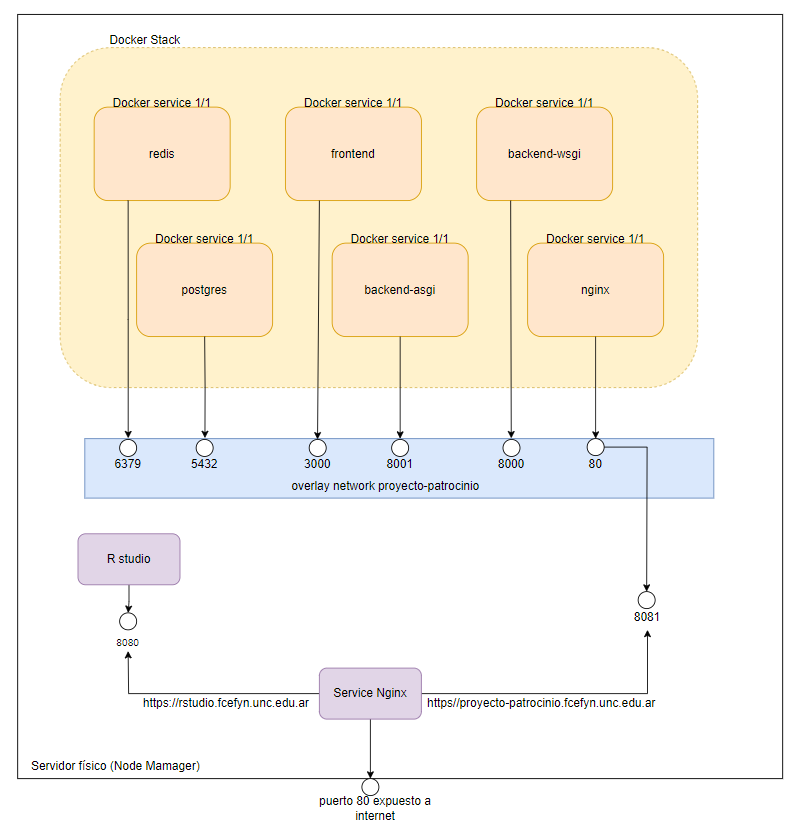
\includegraphics[width=1\linewidth]{fig/deploy.png}
\caption{Diagrama de Despliegue}
\label{fig:deploy-in-server}
\end{figure}

\section{Configuración}

Una vez que la plataforma esté en funcionamiento, el administrador debe acceder al panel web utilizando las credenciales proporcionadas en el archivo de configuración. A continuación, se describen los pasos para realizar la configuración inicial:

\begin{enumerate}
    \item Inicie sesión en la plataforma como administrador.
    \item Ingrese a la siguiente URL: \url{http://{{dominio}}/admin}.
    
    \item Verifique la configuración del dominio en la sección de sitios (Figura \ref{fig:config-sites}). Es esencial asegurarse de que el dominio esté correctamente establecido. Si es necesario realizar cambios, es \textbf{importante}\textbf{ no crear nuevos sitios ni eliminar} el existente, sino editar la información del sitio existente.
\end{enumerate}

\begin{figure}[H]
    \centering
    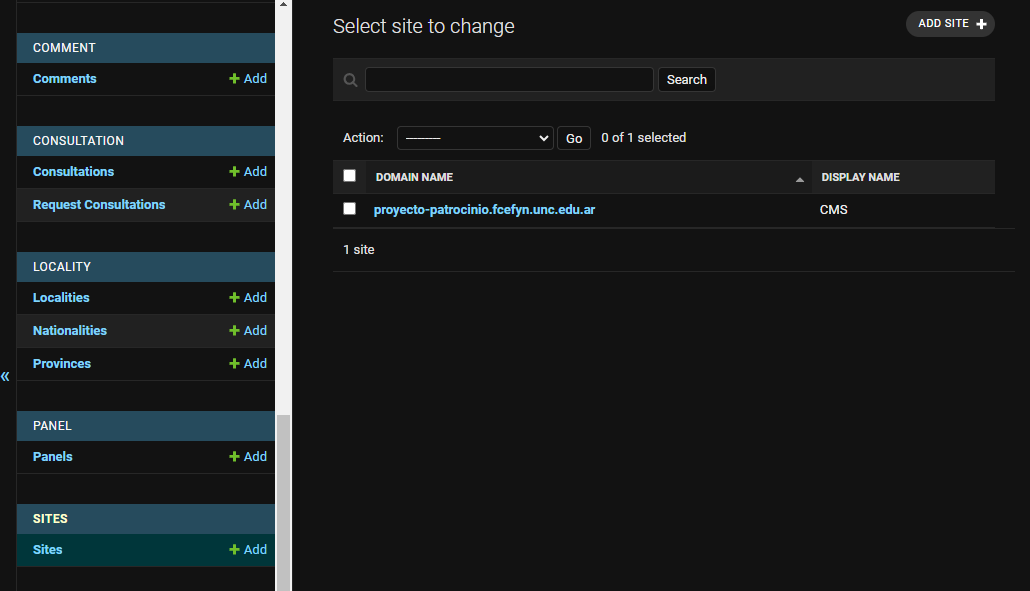
\includegraphics[width=1\linewidth]{fig/sites.png}
    \caption{Configuración de Sitios en el Panel de Administración.}
    \label{fig:config-sites}
\end{figure}


A continuación, el administrador debe crear todas las pizarras de trabajo para cada comisión existente en el patrocinio a través de la sección de \textit{Boards}.

\begin{figure}[H]
    \centering
    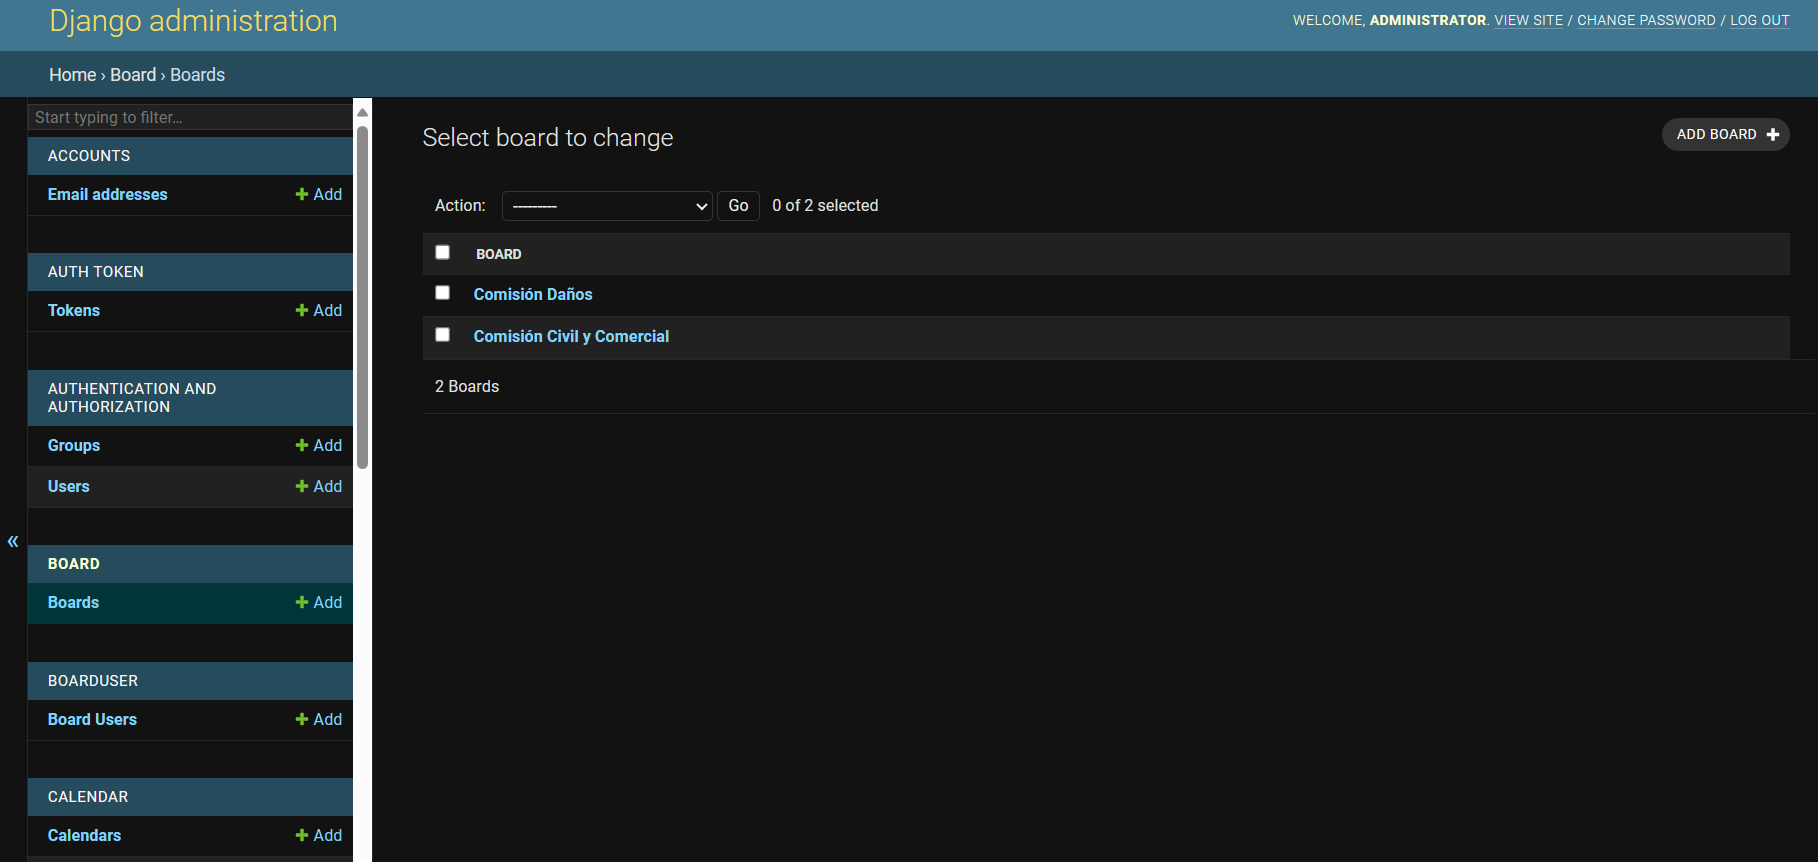
\includegraphics[width=1\linewidth]{fig/boards-admin.png}
    \caption{Creación de Pizarras en la Sección de Administración.}
    \label{fig:boards-admin}
\end{figure}

Finalmente, se deberá registrar una cuenta de usuario para la integración con Google Forms y otorgarle permisos de ``forms''. Para obtener información detallada sobre cómo realizar estos pasos, consulte la sección \ref{sec:registrar-cuenta} para la creación de la cuenta y la sección \ref{subsec:integracion-google-form} para la integración de la cuenta con Google Forms.



\section{Registro de Usuarios}\label{sec:registrar-cuenta}

Para poder registrar un usuario, El usuario deberá seguir los siguientes pasos:

\begin{enumerate}
    \item Ingresar a la página web y seleccionar la opción ``Don't have an account? Sign Up''.
    \item Completar los datos requeridos, acepte los términos y condiciones, y haga clic en el botón ``Sign up''.


    \begin{figure}[H]
        \centering
        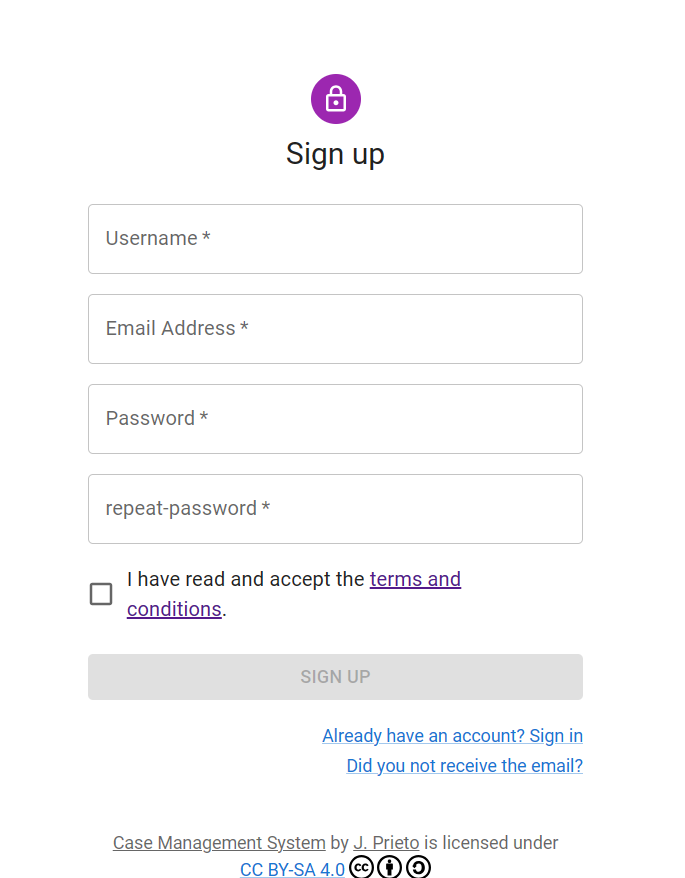
\includegraphics[width=0.7\linewidth]{fig/signup.png}
        \caption{Pantalla de Registro de Usuarios.}
        \label{fig:signup}
    \end{figure}

    \item Revisar la casilla de correlo electrónico y seleccionar el enlace en el correo enviado.

    \textbf{Nota}: El formato de este email, fue previamente configurado con los templates en la etapa de configuración de software.

    \begin{figure}[H]
        \centering
        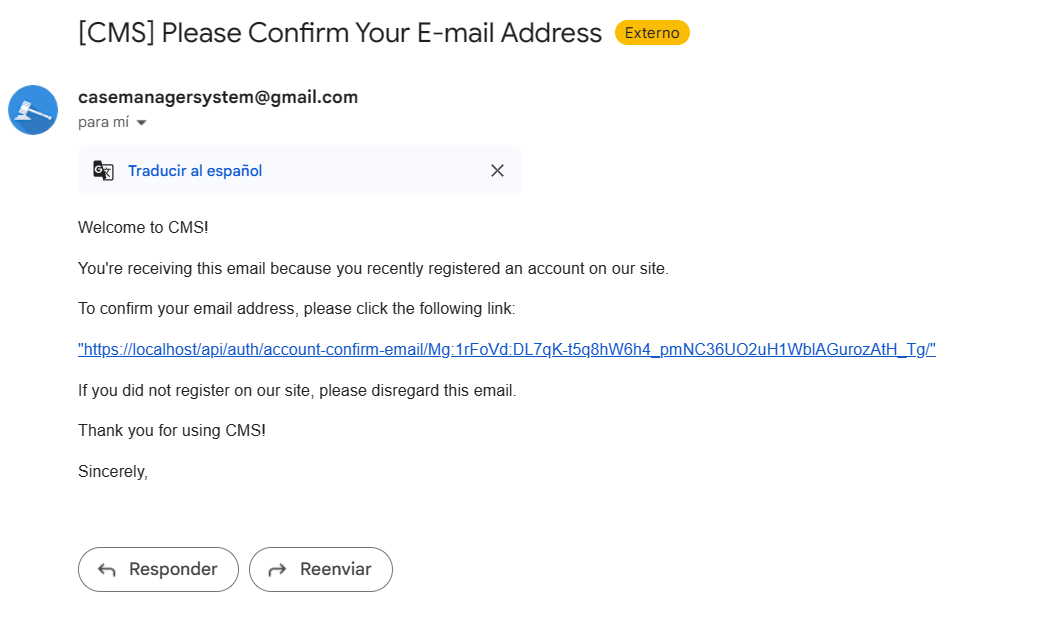
\includegraphics[width=1\linewidth]{fig/confirm-email.png}
        \caption{Confirmación por Correo Electrónico.}
        \label{fig:confirm-email}
    \end{figure}
\end{enumerate}
La página lo redirigirá a la principal, pero aún el usuario no podrá acceder hasta que un administrador habilite su cuenta. Para activar la cuenta, el administrador debe seguir estos pasos:

\begin{enumerate}
    \item Ingresar a la sección de administración y dirigirse a la pestaña de usuarios.
    \item Seleccionar el nuevo usuario y editar la sección de permisos.


    \begin{figure}[H]
        \centering
        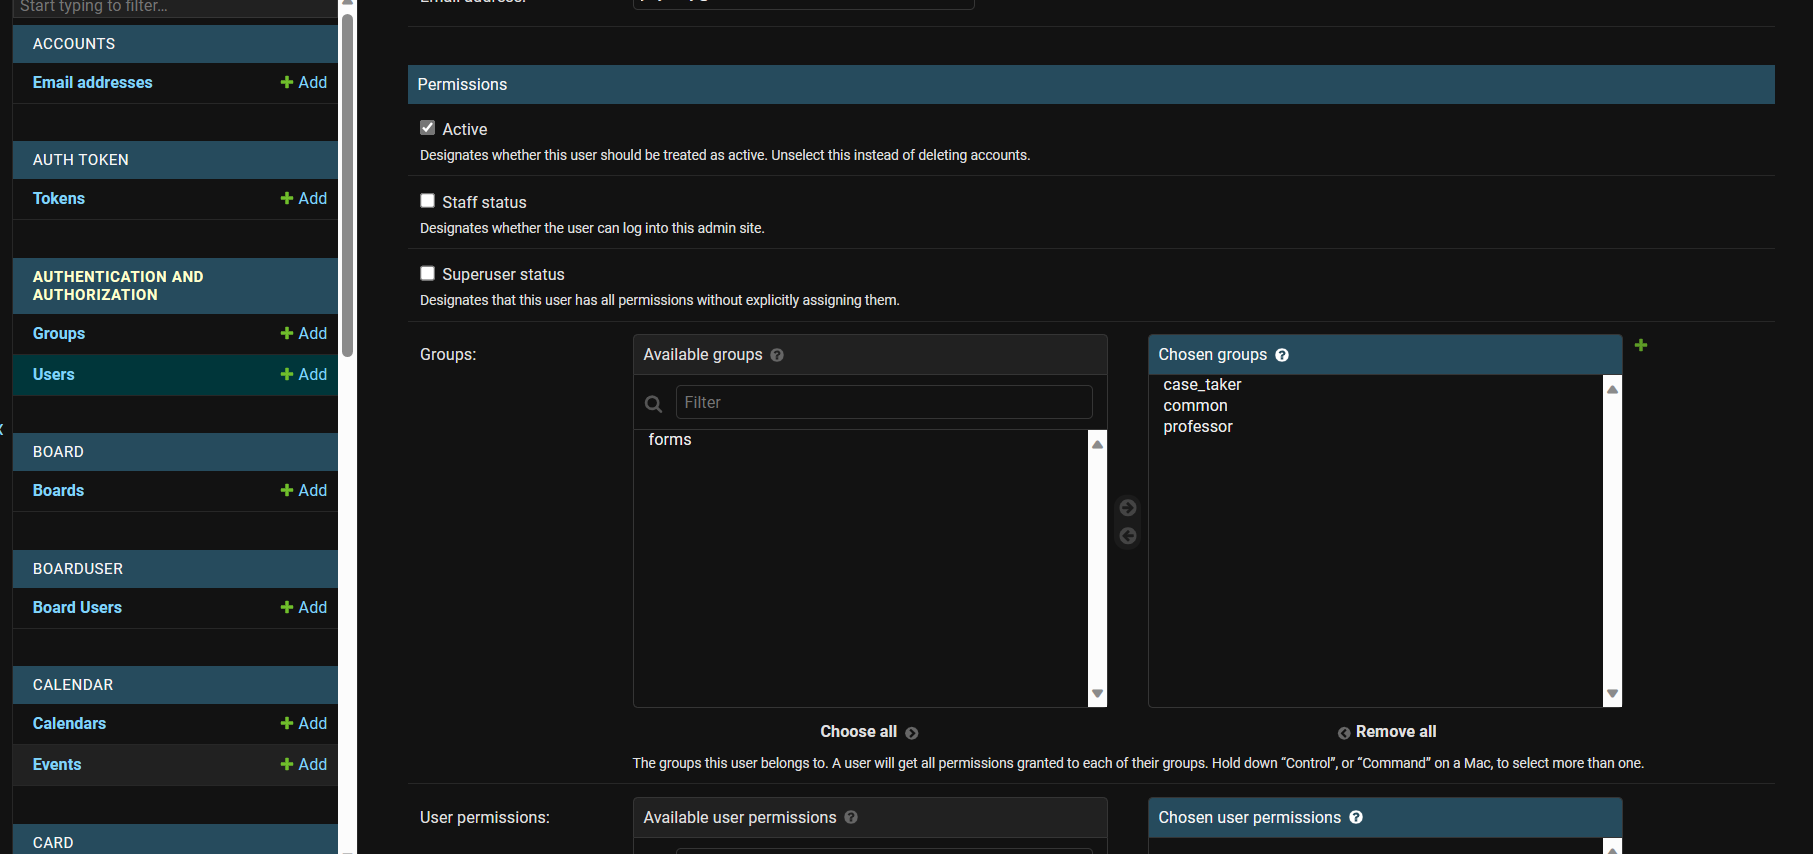
\includegraphics[width=1\linewidth]{fig/user-permission.png}
        \caption{Configuración de Permisos de Usuario.}
        \label{fig:user-permission}
    \end{figure}
    
    \item En la sección, marcar la opción ``Active'' y otorgar los permisos necesarios (ver \ref{sec:permisos-usuarios}) antes de guardar.

\end{enumerate}

Si el usuario es un miembro de una comisión, el administrador también deberá realizar los siguientes pasos adicionales.

\begin{enumerate}
    \item Ingresar a la sección ``Board Users''.
    \item Crear la relación del usuario con la comisión correspondiente.

    \begin{figure}[H]
        \centering
        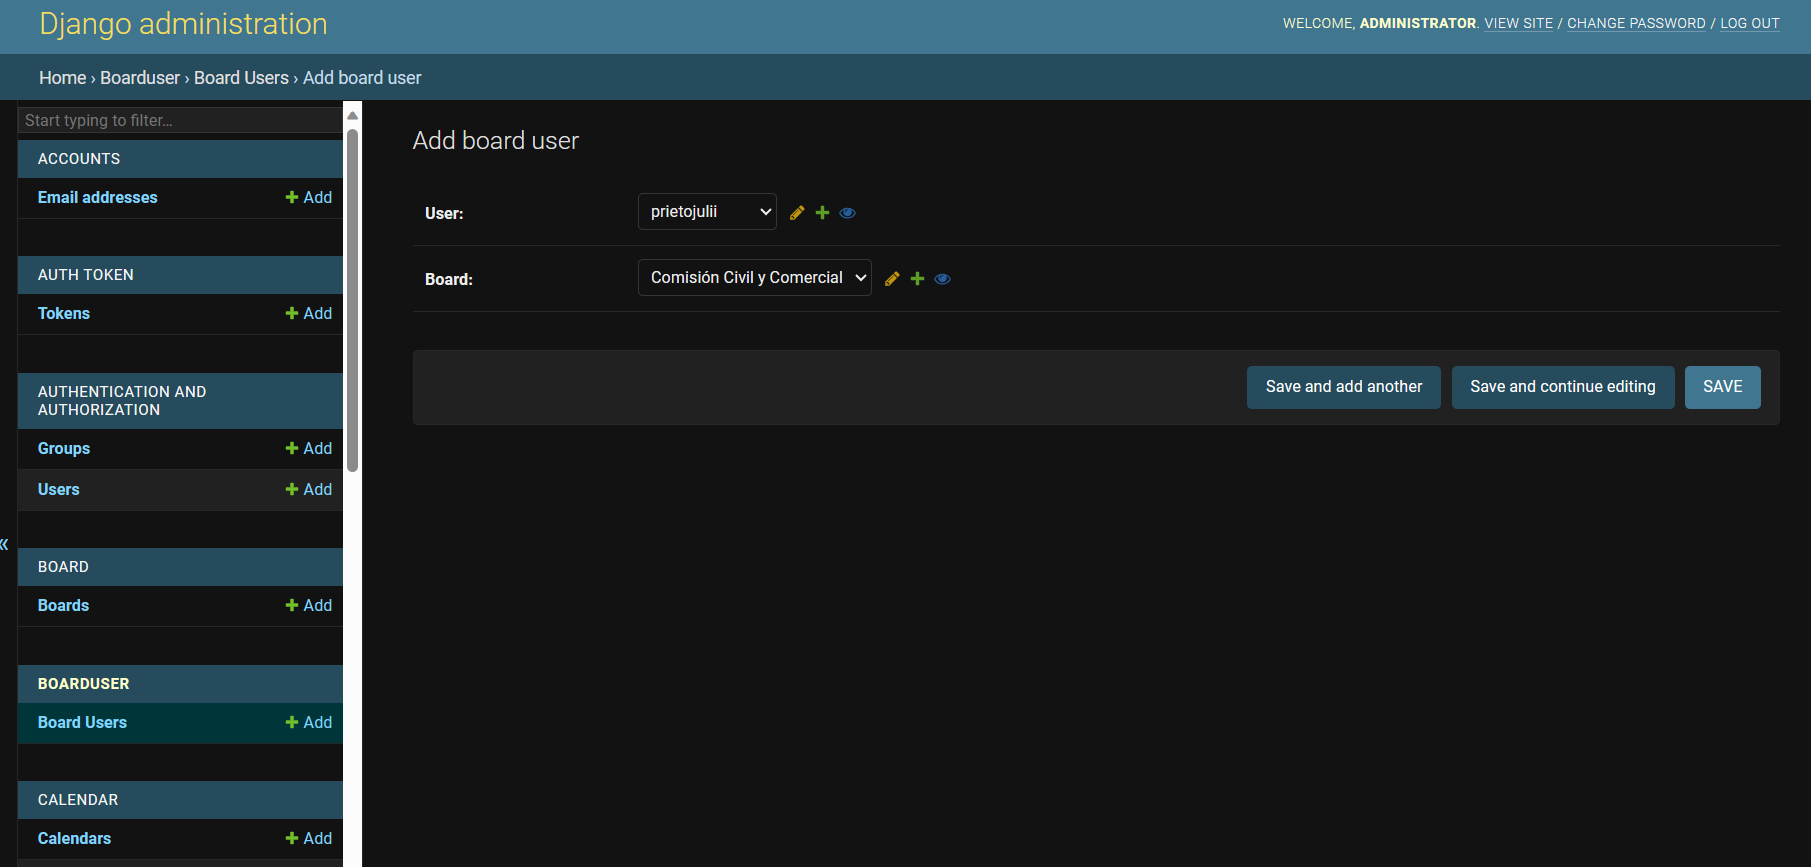
\includegraphics[width=1\linewidth]{fig/board-user.png}
        \caption{Creación de Relación Usuario-Comisión.}
        \label{fig:board-user}
    \end{figure}
    
    \begin{figure}[H]
        \centering
        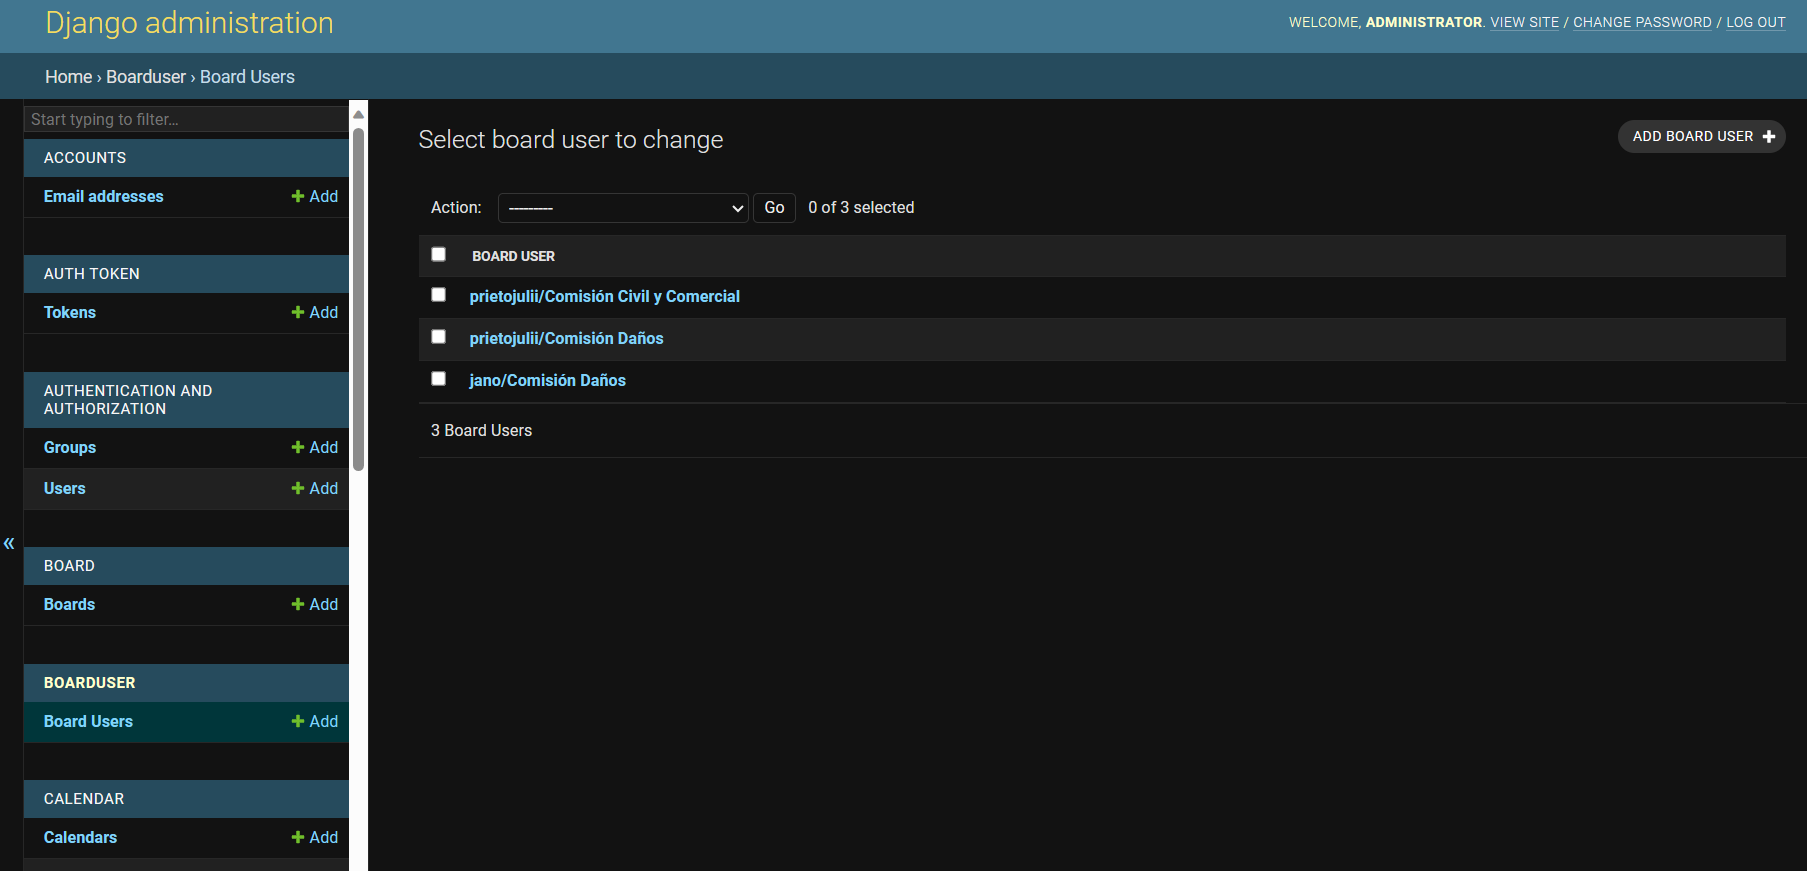
\includegraphics[width=1\linewidth]{fig/board-user-2.png}
        \caption{Lista de Relaciones Usuario-Comisión.}
        \label{fig:board-user-2}
    \end{figure}
\end{enumerate}

Después de completar estos pasos, el usuario podrá iniciar sesión correctamente en la web desde la página de inicio de sesión.

\begin{figure}[H]
    \centering
    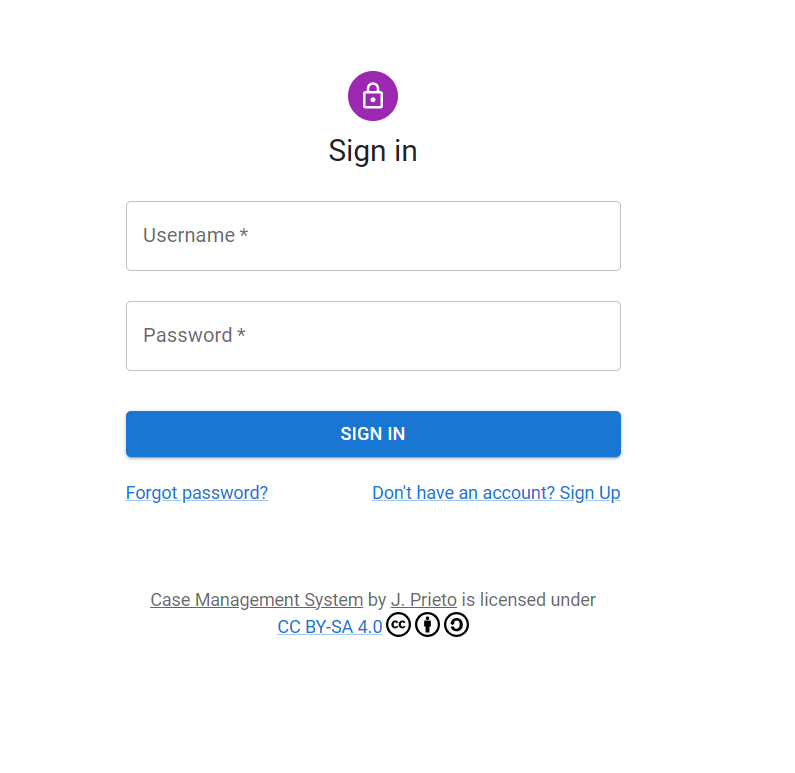
\includegraphics[width=0.7\linewidth]{fig/signin-real-page.png}
    \caption{Página de Inicio de Sesión.}
    \label{fig:signin-real-page-2}
\end{figure}



\section{Permisos de Usuario}\label{sec:permisos-usuarios}

Los grupos de permisos de usuarios se encuentran en la sección "Groups" de la página de administración y se detallan a continuación:

\begin{table}[H]
    \centering
    \begin{tabular}{|c|p{10cm}|}
        \hline
        \textbf{Grupo} & \textbf{Descripción}\\
        \hline
        common & Grupo de permisos básicos necesarios tanto para un tomador de caso como para un profesor.\\
        \hline
        case\_taker & Grupo de permisos para un tomador de caso. Necesarios para el manejo de la consultoría.\\
        \hline
        professor & Grupo de permisos para un profesor. Necesarios para el manejo de una comisión.\\
        \hline
        forms & Grupo de permisos exclusivo para la cuenta de Google Forms, que le permite registrar formularios.\\
        \hline
    \end{tabular}
    \caption{Grupos de Permisos de Usuario.}
    \label{tab:grupos-permisos-usuario}
\end{table}

\section{Permisos de Usuario}\label{sec:permisos-usuarios}

Los grupos de permisos de usuarios se encuentran en la sección "Groups" de la página de administración y se detallan a continuación:

\begin{table}[H]
    \centering
    \begin{tabular}{|c|p{10cm}|}
        \hline
        \textbf{Grupo} & \textbf{Descripción}\\
        \hline
        common & Grupo de permisos básicos necesarios tanto para un tomador de caso como para un profesor.\\
        \hline
        case_taker & Grupo de permisos para un tomador de caso. Necesarios para el manejo de la consultoría.\\
        \hline
        professor & Grupo de permisos para un profesor. Necesarios para el manejo de una comisión.\\
        \hline
        forms & Grupo de permisos exclusivo para la cuenta de Google Forms, que le permite registrar formularios.\\
        \hline
    \end{tabular}
    \caption{Grupos de Permisos de Usuario.}
    \label{tab:grupos-permisos-usuario}
\end{table}

\textbf{Nota:} El grupo de permisos \textit{common} debe asignarse junto con \textit{case\_taker} o \textit{professor}.


\section{Administración}\label{sec:administracion}

La página de administración proporciona una interfaz amigable para visualizar y gestionar todos los datos del sistema. Al ingresar a la página principal, se presenta una disposición organizada de los datos agrupados en secciones. Además, a la derecha, se muestra un historial de acciones recientes.

\begin{figure}[H]
    \centering
    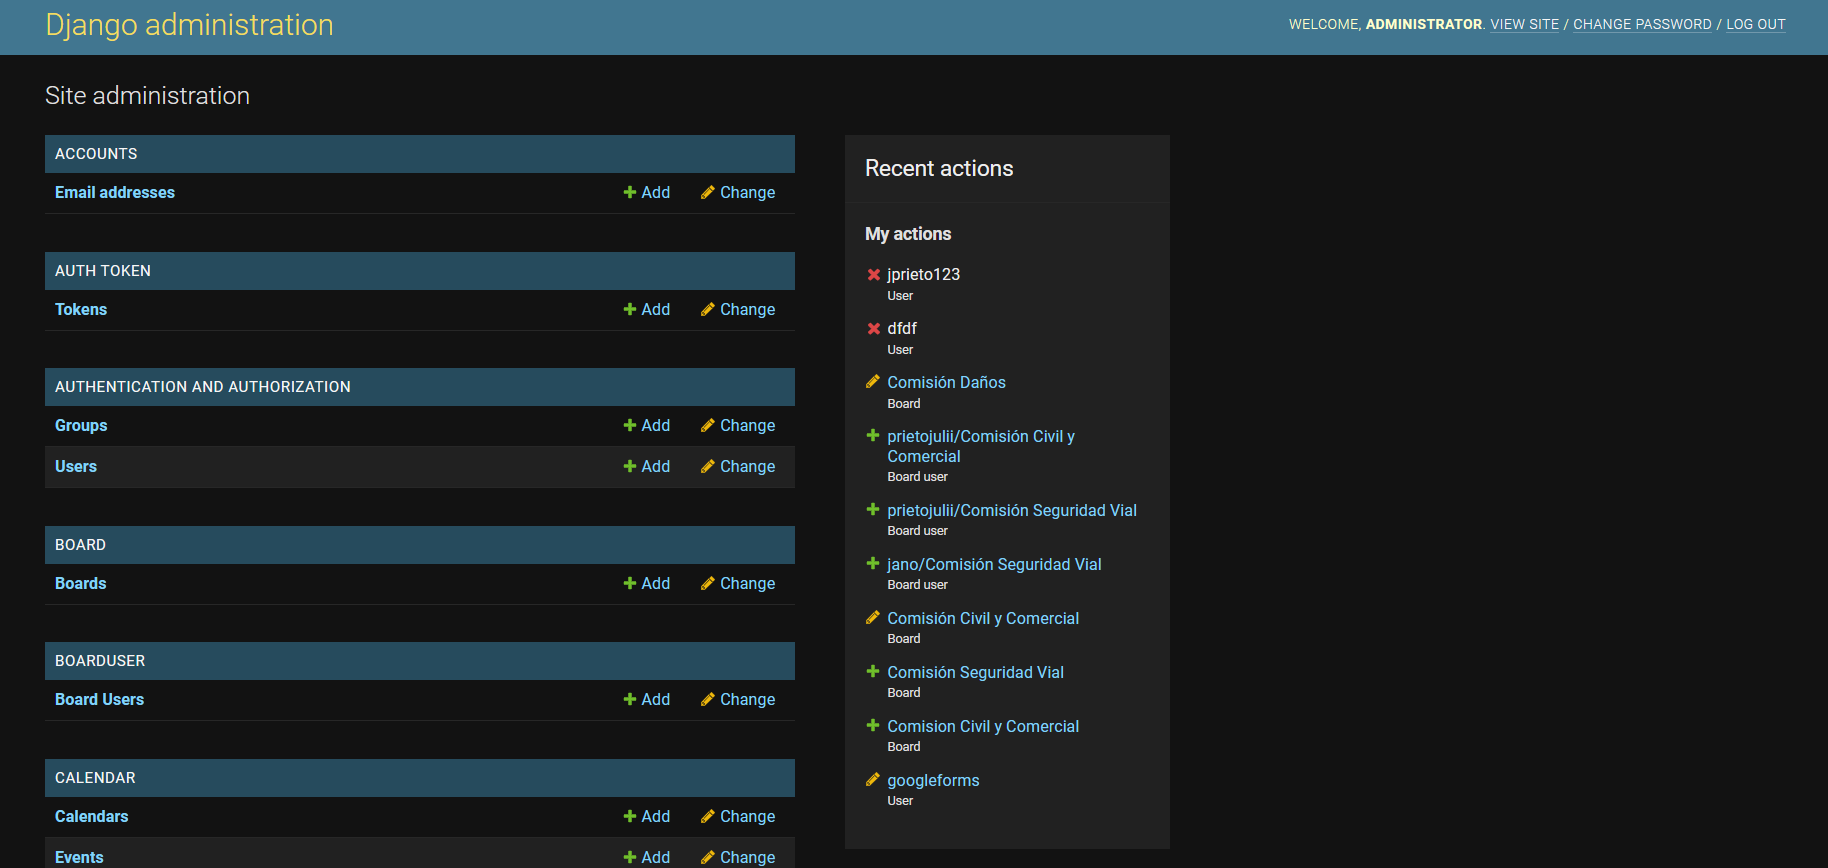
\includegraphics[width=1\linewidth]{fig/administracion.png}
    \caption{Interfaz de Administración de Django.}
    \label{fig:admin-interface}
\end{figure}

En esta interfaz, los administradores pueden realizar diversas acciones, como agregar, editar o eliminar registros, administrar permisos de usuario y conocer el estado del sistma.



\section{Tablero de Trabajo de Consultoría}
La página de consultoría es responsable de la administración de las consultas. Aquí, los tomadores de casos pueden revisar las consultas entrantes, representadas como tickets generados a través de formularios de Google. Pueden analizarlas y verificar si cumplen con las condiciones para ser patrocinadas por la entidad. Los tomadores de casos tienen la capacidad de crear, editar y eliminar consultas o enviarlas a una comisión para solicitar patrocinio.

La página está estructurada mediante paneles. El panel izquierdo contiene las consultas sin asignar, mientras que los paneles siguientes representan comisiones, cada uno con los tickets de las solicitudes de asignación. Para asignar una consulta a una comisión, basta con arrastrar la consulta al tablero de la comisión deseada. También es posible eliminar la solicitud volviendo a arrastrar el ticket al panel izquierdo. Para eliminar el ticket, simplemente posicione el mouse sobre el mismo, seleccione el menú que aparecerá y elija la opción "delete".

\begin{figure}[H]
    \centering
    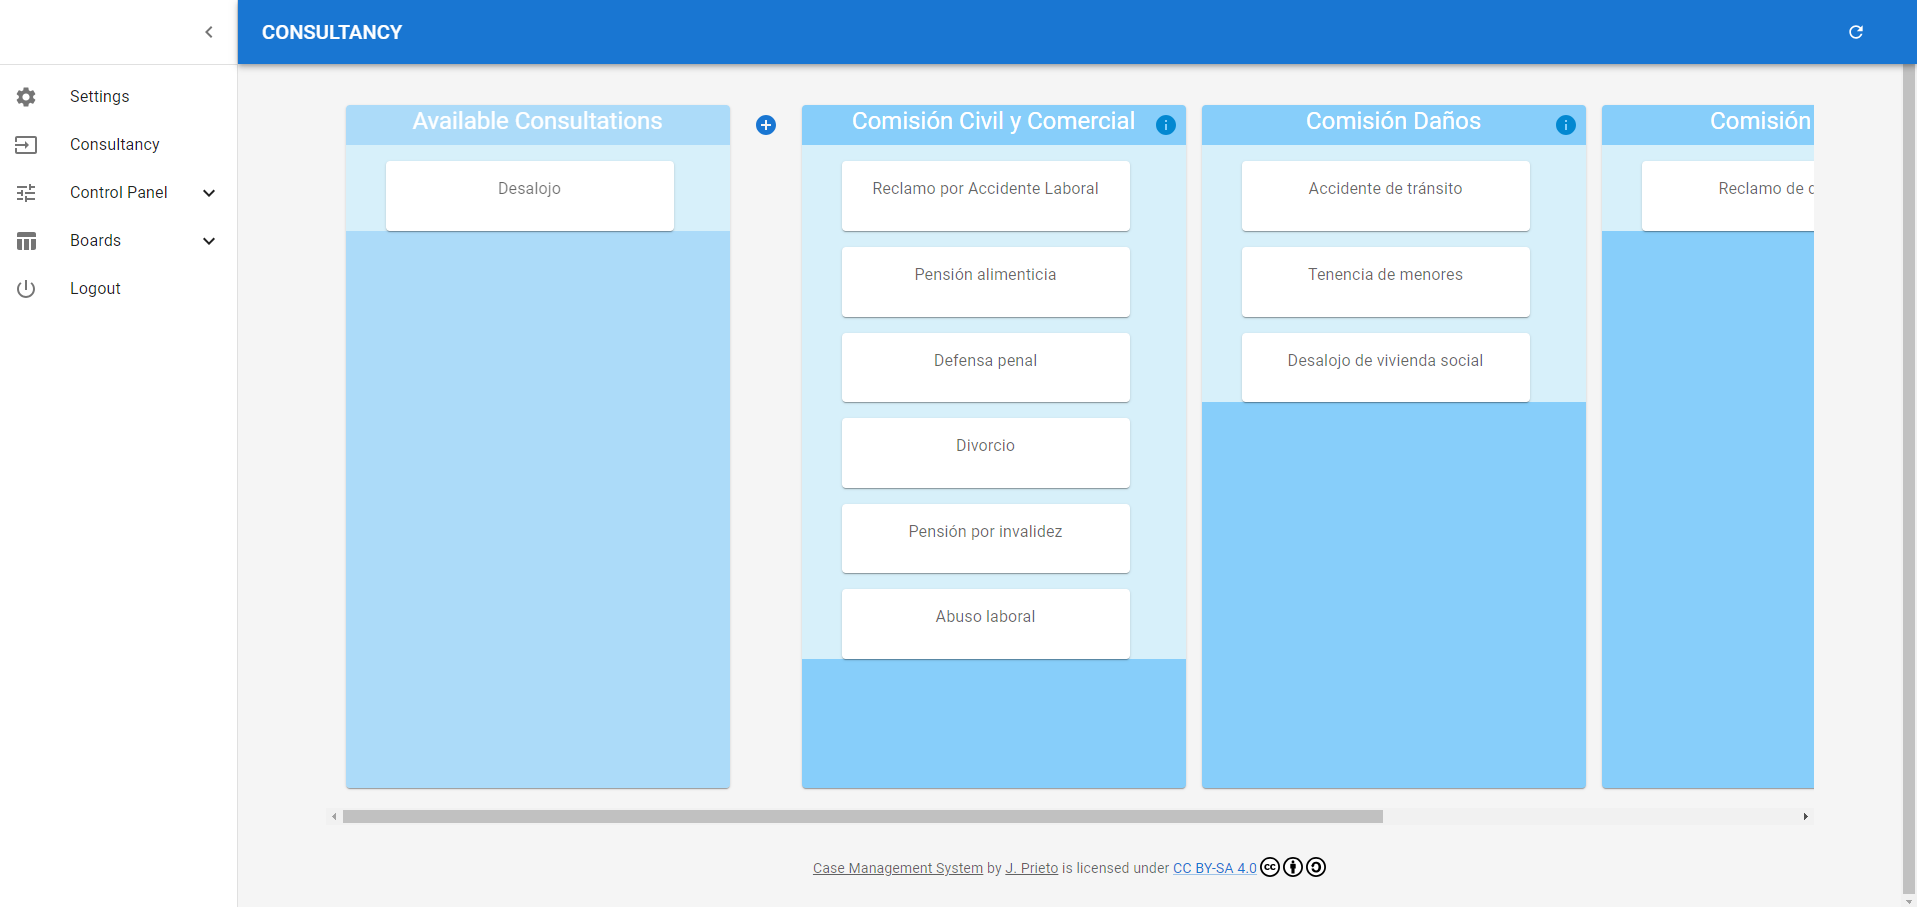
\includegraphics[width=1\linewidth]{fig/consultancy-real-page.png}
    \caption{Página de Consultoría}
    \label{fig:consultancy-real-page}
\end{figure}

Es importante mantener un registro del estado de cada comisión. Cada panel cuenta con un popper en el sector superior derecho que, al hacer clic, muestra la cantidad de consultas asignadas y la cantidad de consultas por estado (por hacer, en progreso o pausadas/bloqueadas). Además, incluye un historial de las asignaciones de los últimos 10 días, que muestra el ``tag'' de la consulta y la fecha de asignación.

\begin{figure}[H]
    \centering
    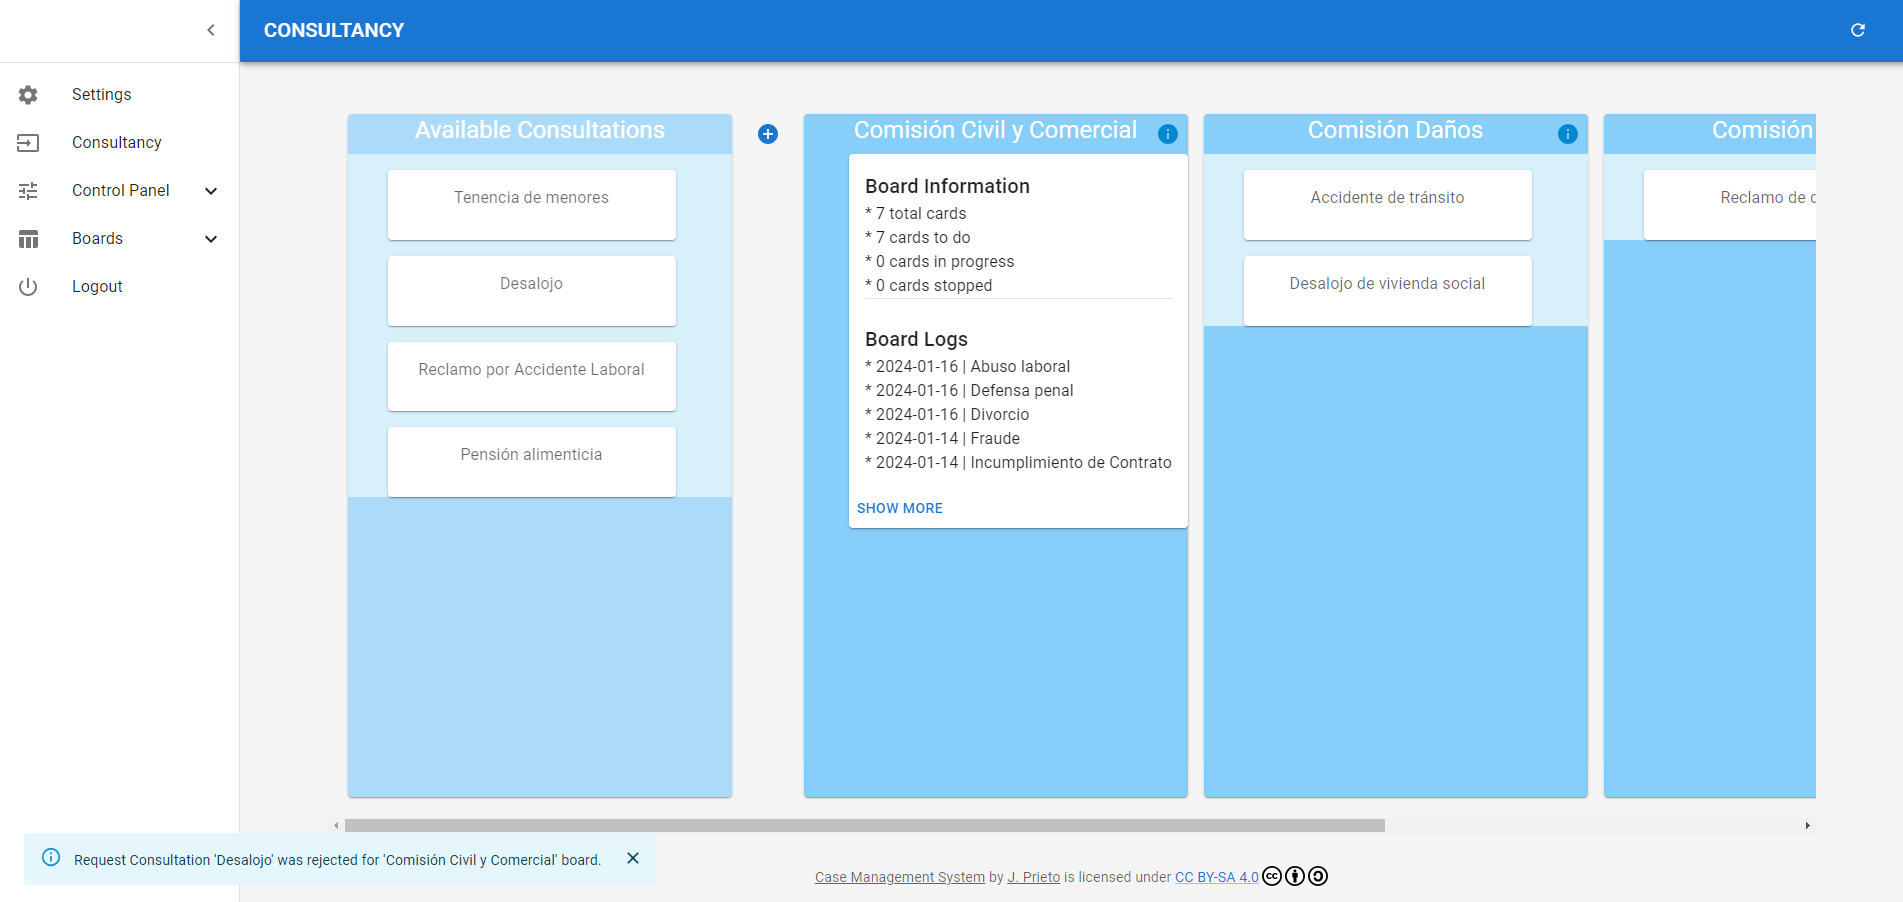
\includegraphics[width=1\linewidth]{fig/consultancy-real-page-logs-1.png}
    \caption{Historial de Asignaciones de una Comisión}
    \label{fig:consultancy-logs-1}
\end{figure}

Cuando la cantidad de consultas asignadas a la comisión en los últimos 10 días es extensa, aparecerá la opción ``show more'', que expandirá un panel con todas las asignaciones.

\begin{figure}[H]
    \centering
    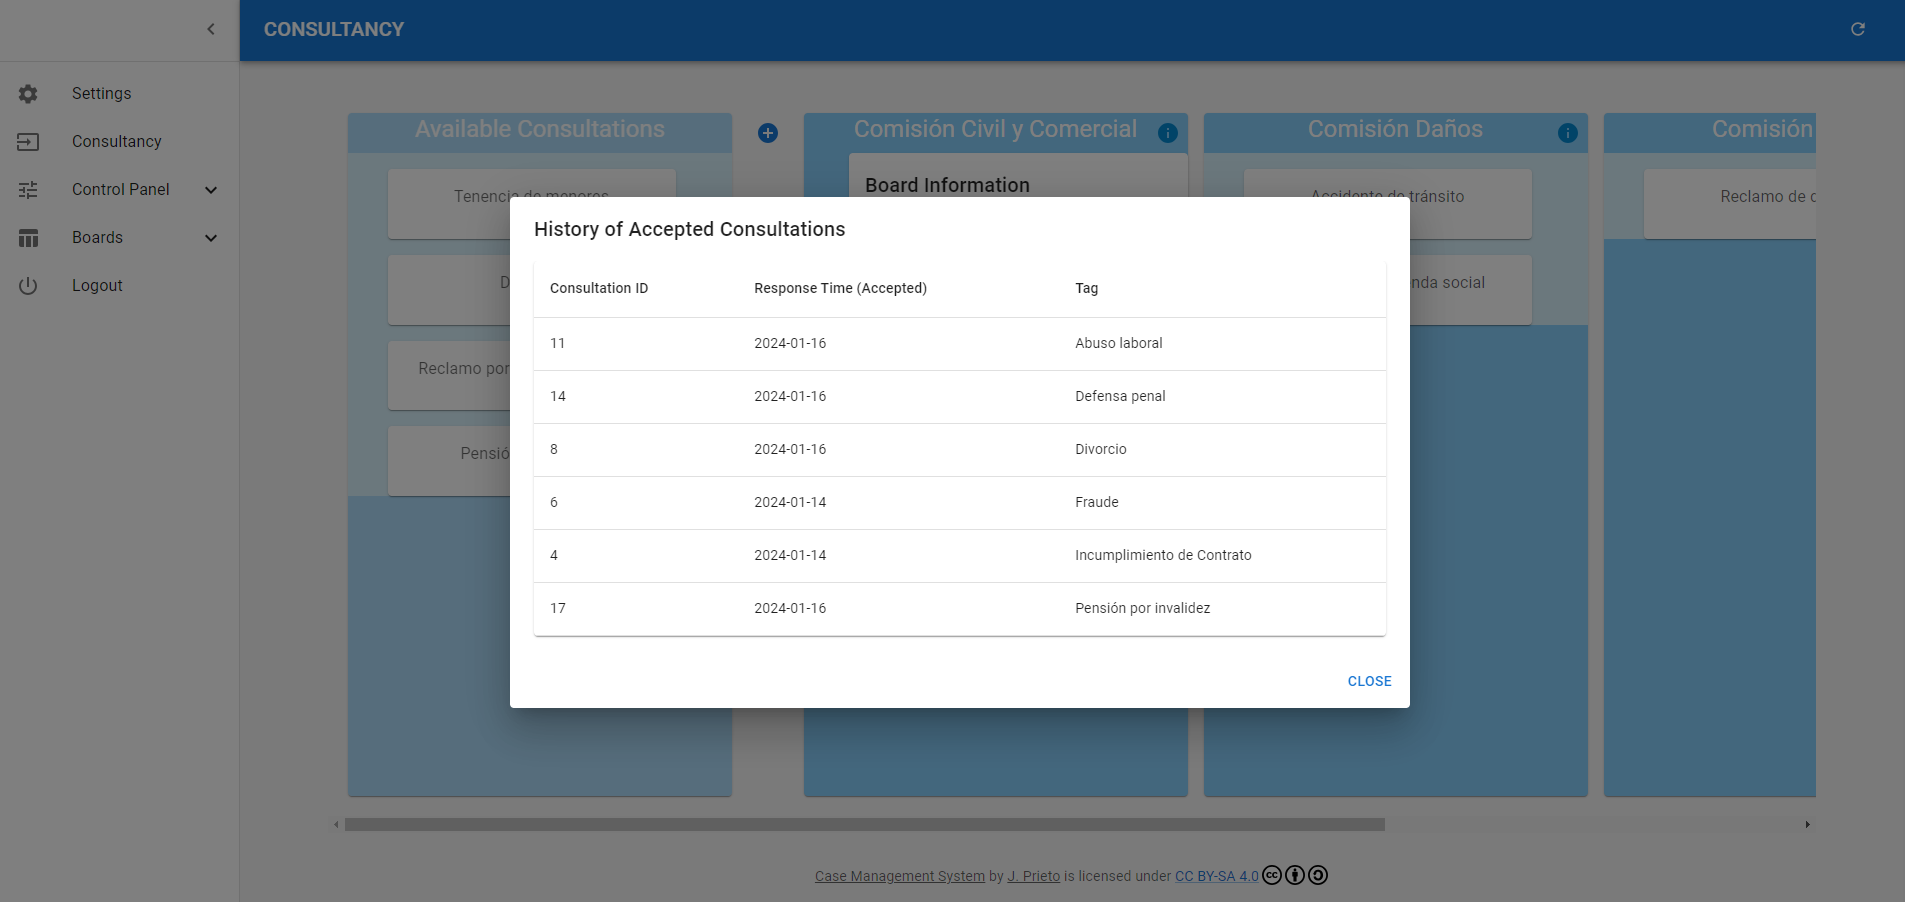
\includegraphics[width=1\linewidth]{fig/consultancy-real-page-logs-2.png}
    \caption{Panel Expandido de Historial de Asignaciones de una Comisión}
    \label{fig:consultancy-logs-2}
\end{figure}

El Usuario Tomador de Caso tiene la capacidad de crear consultas a través de la página de consultoría. Para hacerlo, se selecciona el botón con el símbolo ``+'' ubicado en el panel de entrada, y luego se completa el formulario según se muestra a continuación.

\begin{figure}[H]
    \centering
    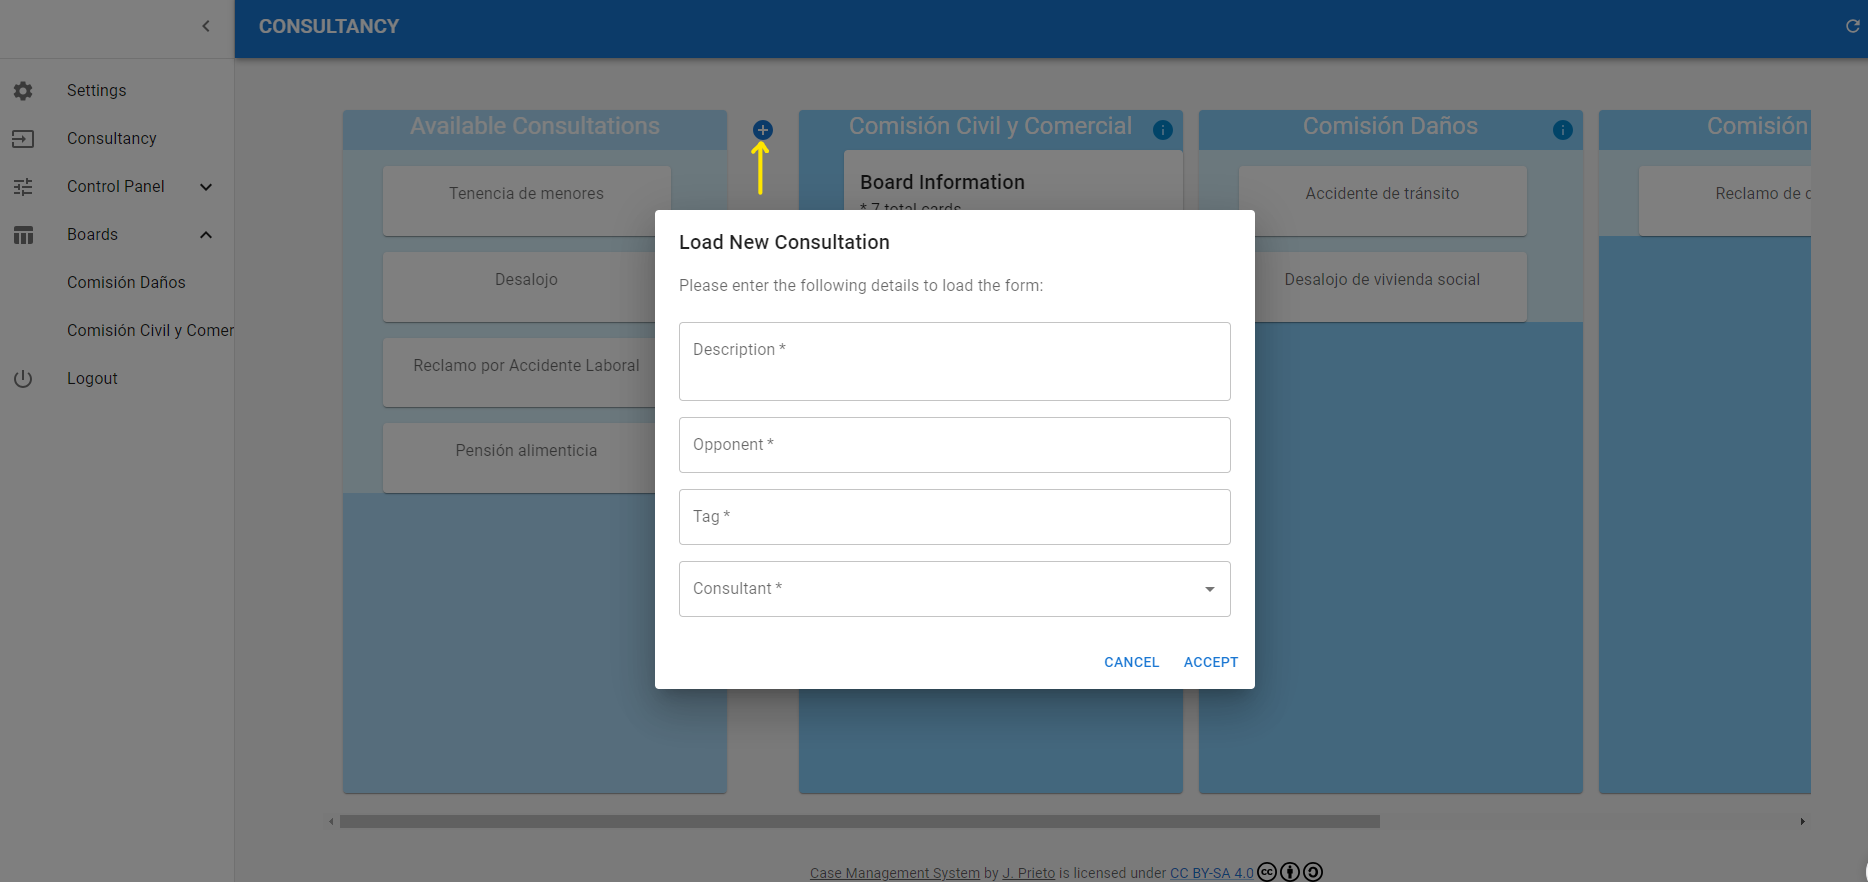
\includegraphics[width=1\linewidth]{fig/crear-consulta-consultancy.png}
    \caption{Formulario para Crear Consulta en la Página de Consultoría}
    \label{fig:formulario-crear-consulta}
\end{figure}




\section{Panel de Control}
El panel de control consta de dos pestañas principales: ``Consultations'' y ``Clients''. Ambas pestañas ofrecen tablas que pueden descargarse en formato PDF o CSV. Además, proporcionan opciones de filtro y permiten la edición, creación o eliminación de registros.

A continuación, se presenta la pestaña de ``Consultations'', que muestra una tabla con todas las consultas.

\begin{figure}[H]
    \centering
    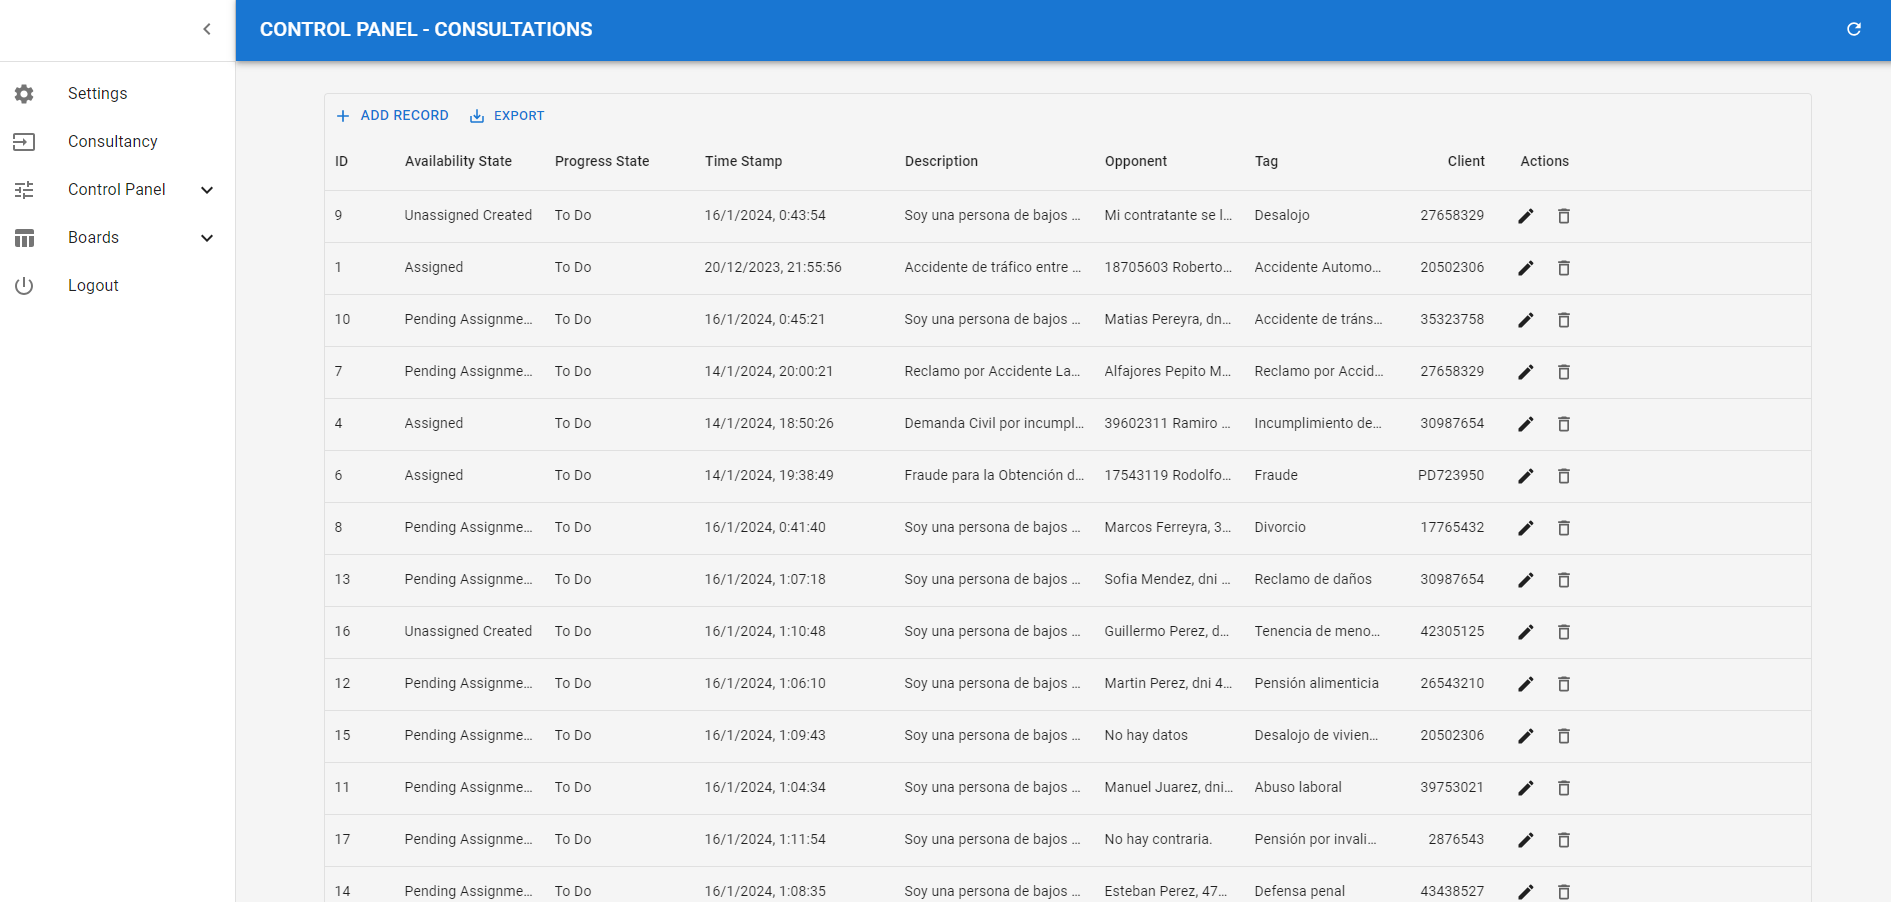
\includegraphics[width=1\linewidth]{fig/consultation-real-page.png}
    \caption{Tabla de Consultas en el Panel de Control.}
    \label{fig:consultations-table}
\end{figure}


A continuación, se presenta la pestaña de ``Clients'', que muestra una tabla con todos los clientes.

\begin{figure}[H]
    \centering
    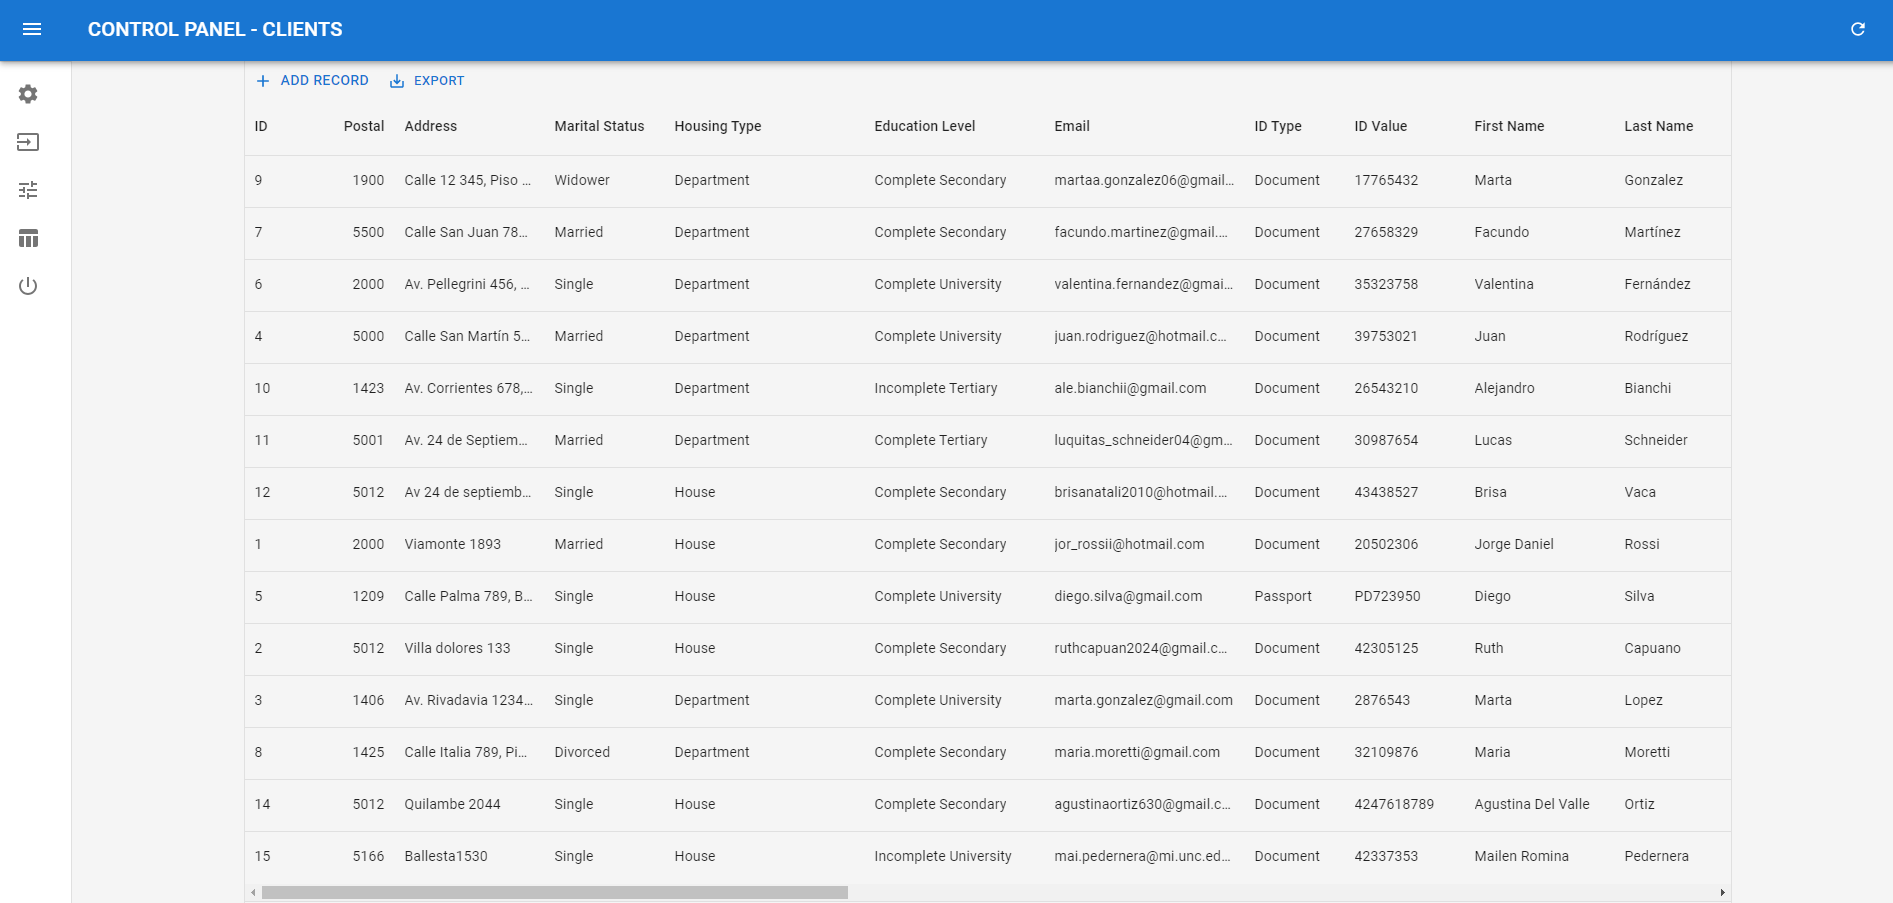
\includegraphics[width=1\linewidth]{fig/clients-real-page.png}
    \caption{Tabla de Clientes en el Panel de Control.}
    \label{fig:clients-table}
\end{figure}

Cada entrada en esta tabla puede ser eliminada o editada seleccionando los elementos en la última columna a la derecha de la entrada deseada. Además, es posible crear un nuevo registro haciendo clic en el botón ``Add Record'' en la parte superior.

La tabla también permite aplicar filtros a algunas de sus columnas. Para ello, cada columna tiene un tooltip que facilita la ordenación ascendente o descendente, filtrado y ocultamiento de la columna. A continuación, se muestra un ejemplo de aplicación de un filtro a la columna ``progress state'' de la tabla ``consultations''.

\begin{figure}[H]
    \centering
    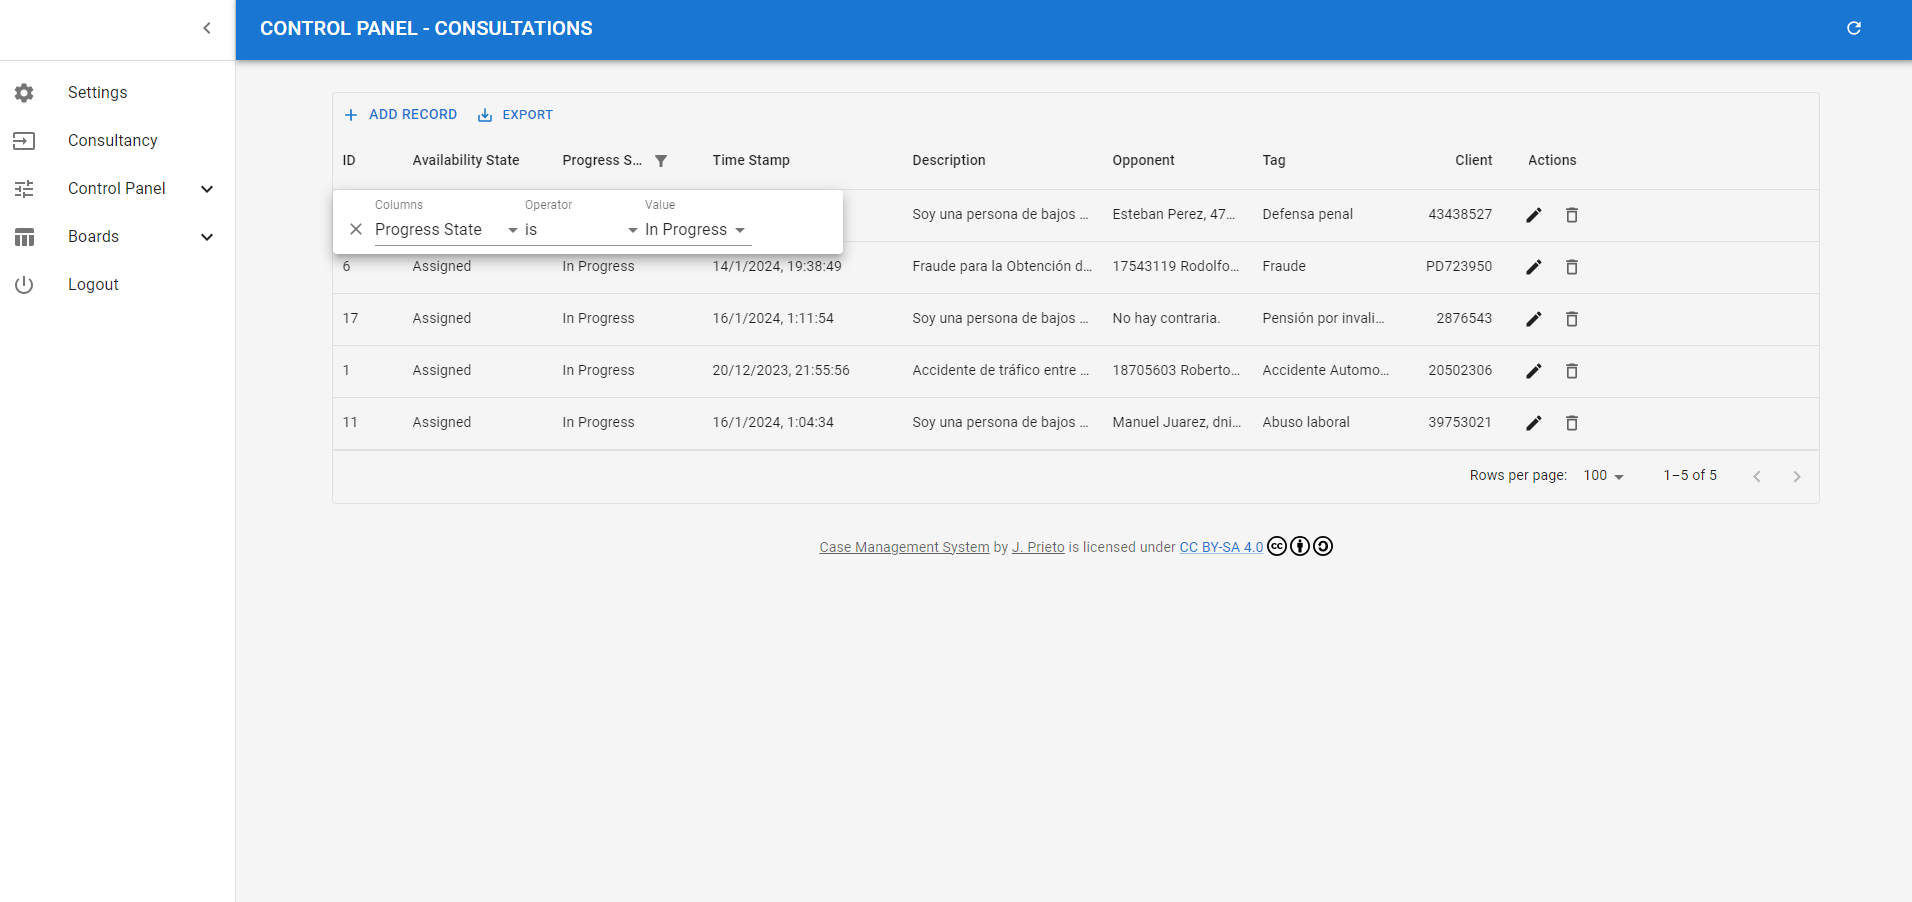
\includegraphics[width=1\linewidth]{fig/tabla-filter.png}
    \caption{Aplicación de un Filtro en la Columna Progress State}
    \label{fig:tabla-filtro-ejemplo}
\end{figure}



\section{Tablero de Trabajo para la Comisión}
Cada comisión cuenta con un ``Board'', el cual los usuarios con acceso podrán visualizar desde la sección ``Boards'' en el menú desplegable de la página.

Este espacio está organizado en paneles, siendo el primero a la izquierda el panel de entrada de solicitudes de asignación de casos. Para aceptar una solicitud, basta con arrastrar el ticket de la consulta a alguno de los paneles internos del board. Para rechazarla, se puede seleccionar la opción ``rejected'' desde el menú del ticket, el cual se hace visible acercando el ratón sobre él.

Los paneles a la izquierda son flexibles y pueden ser creados según la necesidad del usuario, ya sea como organizadores, separadores de consultas, o para cualquier otro agrupamiento conveniente. Por ejemplo, podrían ser utilizados un panel por profesor, otro por estado de progreso de las consultas, o cualquier otro criterio de agrupación preferido.

\begin{figure}[H]
    \centering
    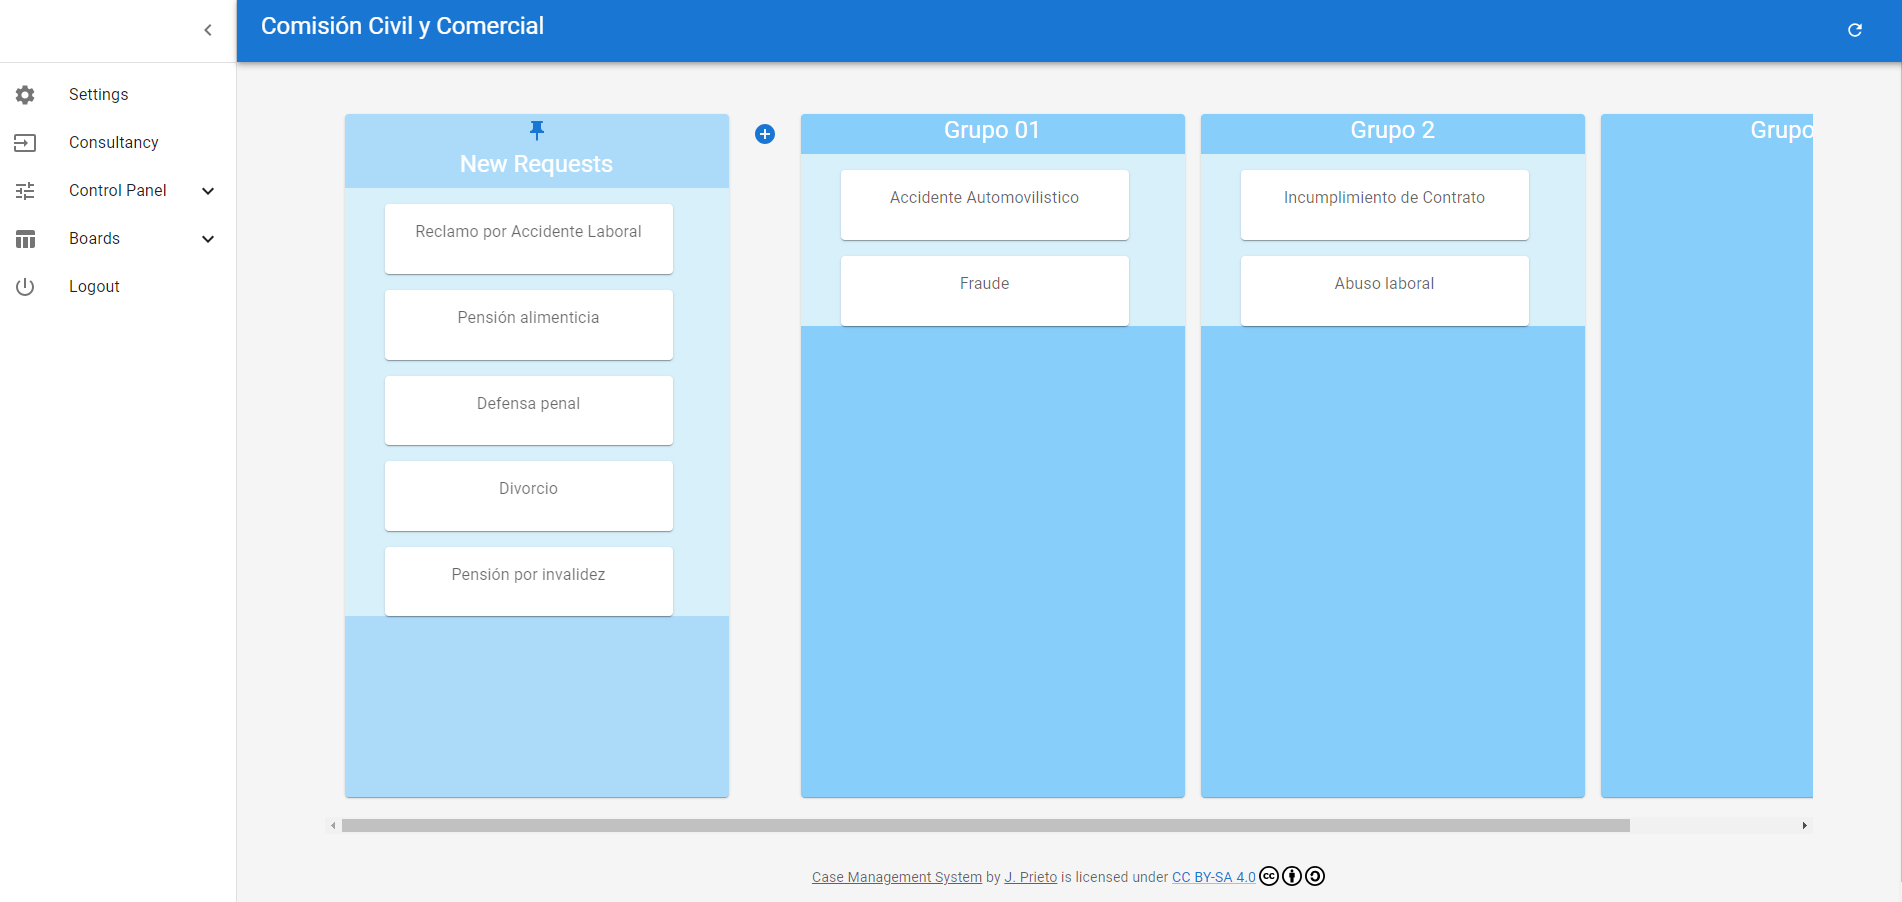
\includegraphics[width=1\linewidth]{fig/board-real-page.png}
    \caption{Página Board de la Comisión}
    \label{fig:board-real-page}
\end{figure}

Cada panel se puede crear utilizando el botón ``+'' e ingresando el nombre correspondiente. Asimismo, se pueden eliminar a través del menú del panel o editar el título haciendo doble clic sobre él (siempre y cuando no existan tickets en el tablero). Además, el board puede ser renombrado haciendo doble clic sobre el título.

\begin{figure}[H]
    \centering
    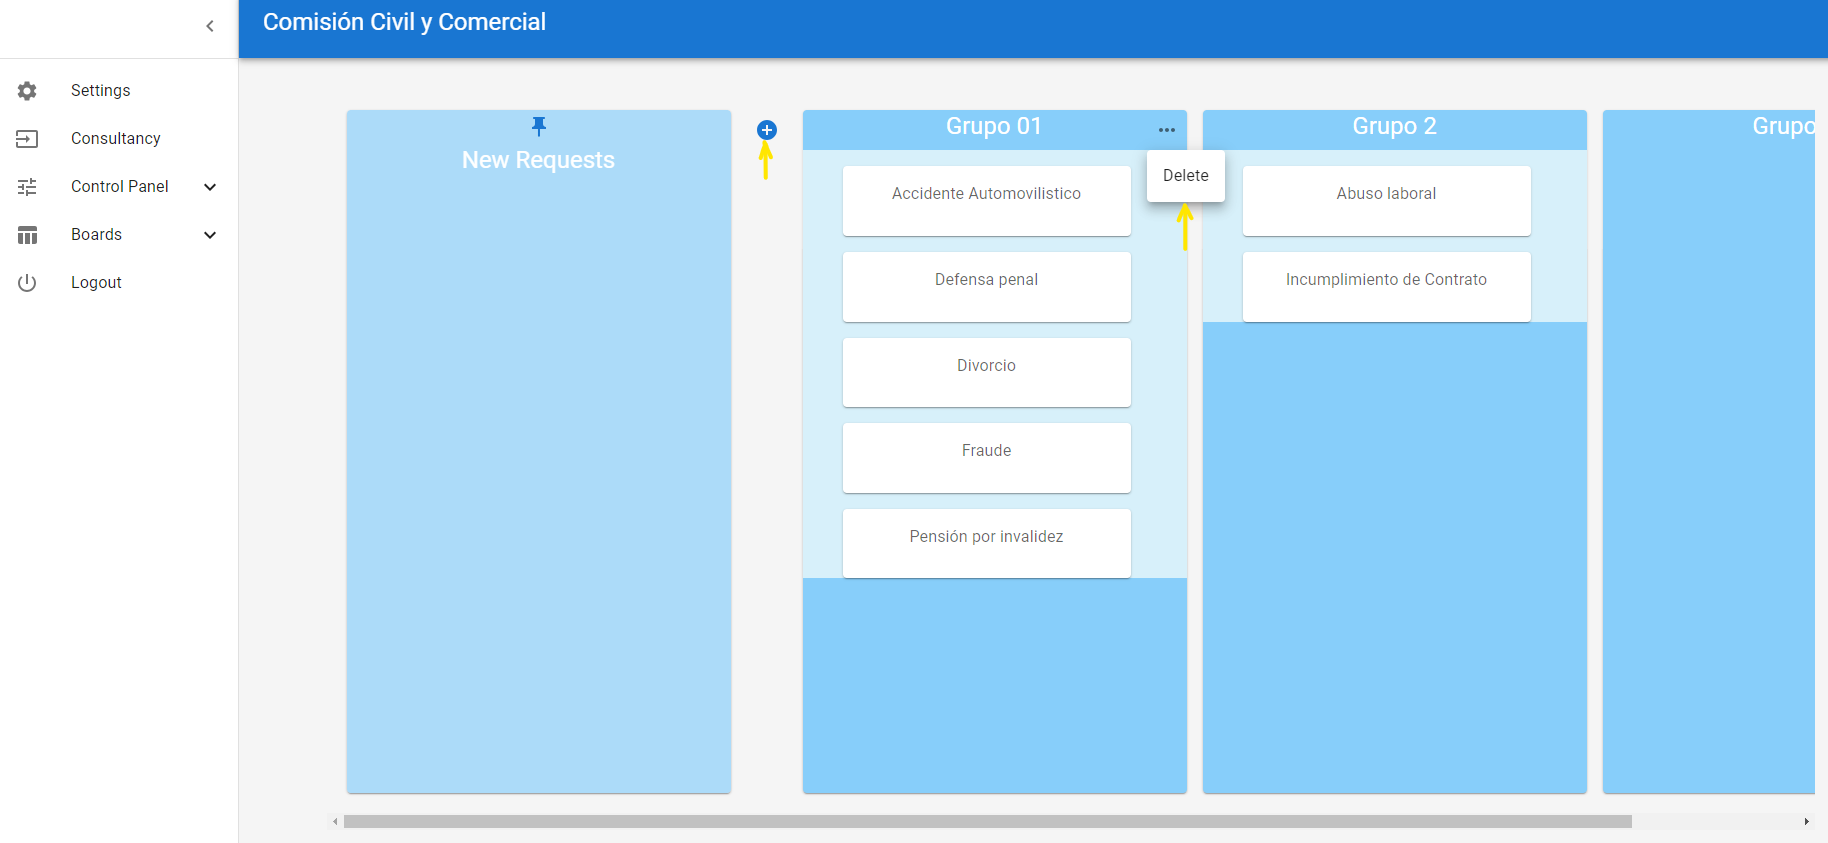
\includegraphics[width=1\linewidth]{fig/delete-panel.png}
    \caption{Botones para eliminar o crear un Panel del Board}
    \label{fig:delete-panel}
\end{figure}





\section{Detalles de la Consulta}\label{sec:info-consulta}

Para obtener más detalles sobre una consulta específica, se debe hacer click en la tarjeta correspondiente, lo que desplegará un cuadro con tres pestañas distintas.

\begin{figure}[H]
    \centering
    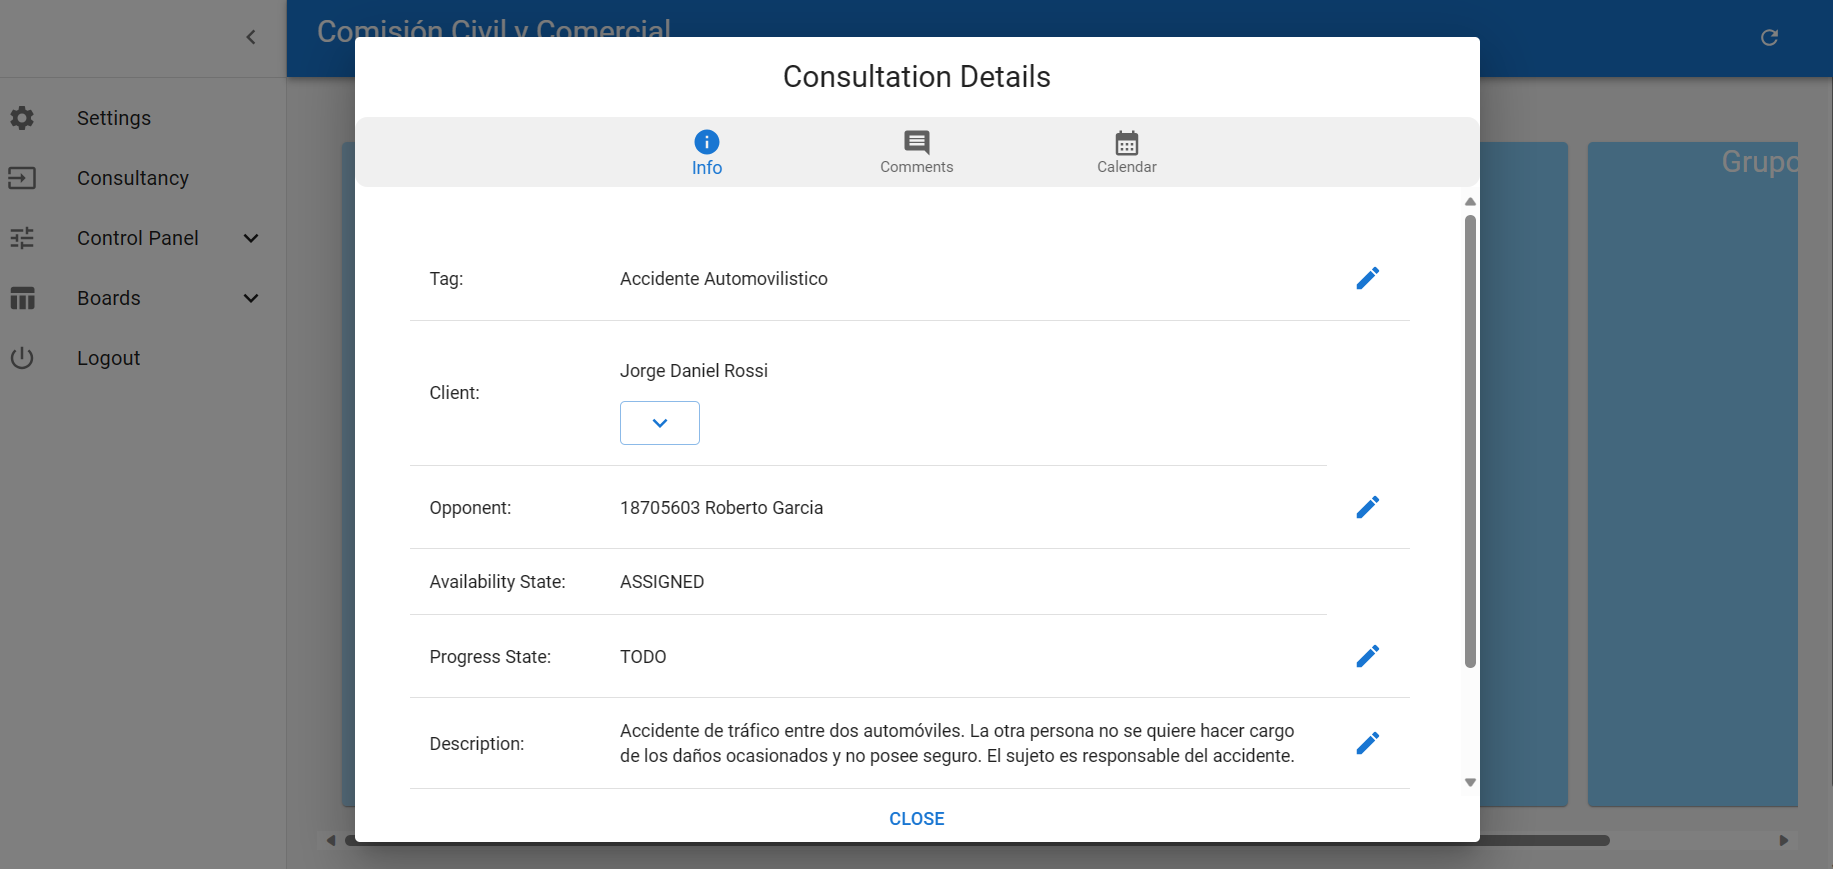
\includegraphics[width=1\linewidth]{fig/info-consulta.png}
    \caption{Ventana de Información de Consulta.}
    \label{fig:consulta-info}
\end{figure}

La primera pestaña presenta información organizada sobre el cliente y los detalles de la consulta.

\begin{figure}[H]
    \centering
    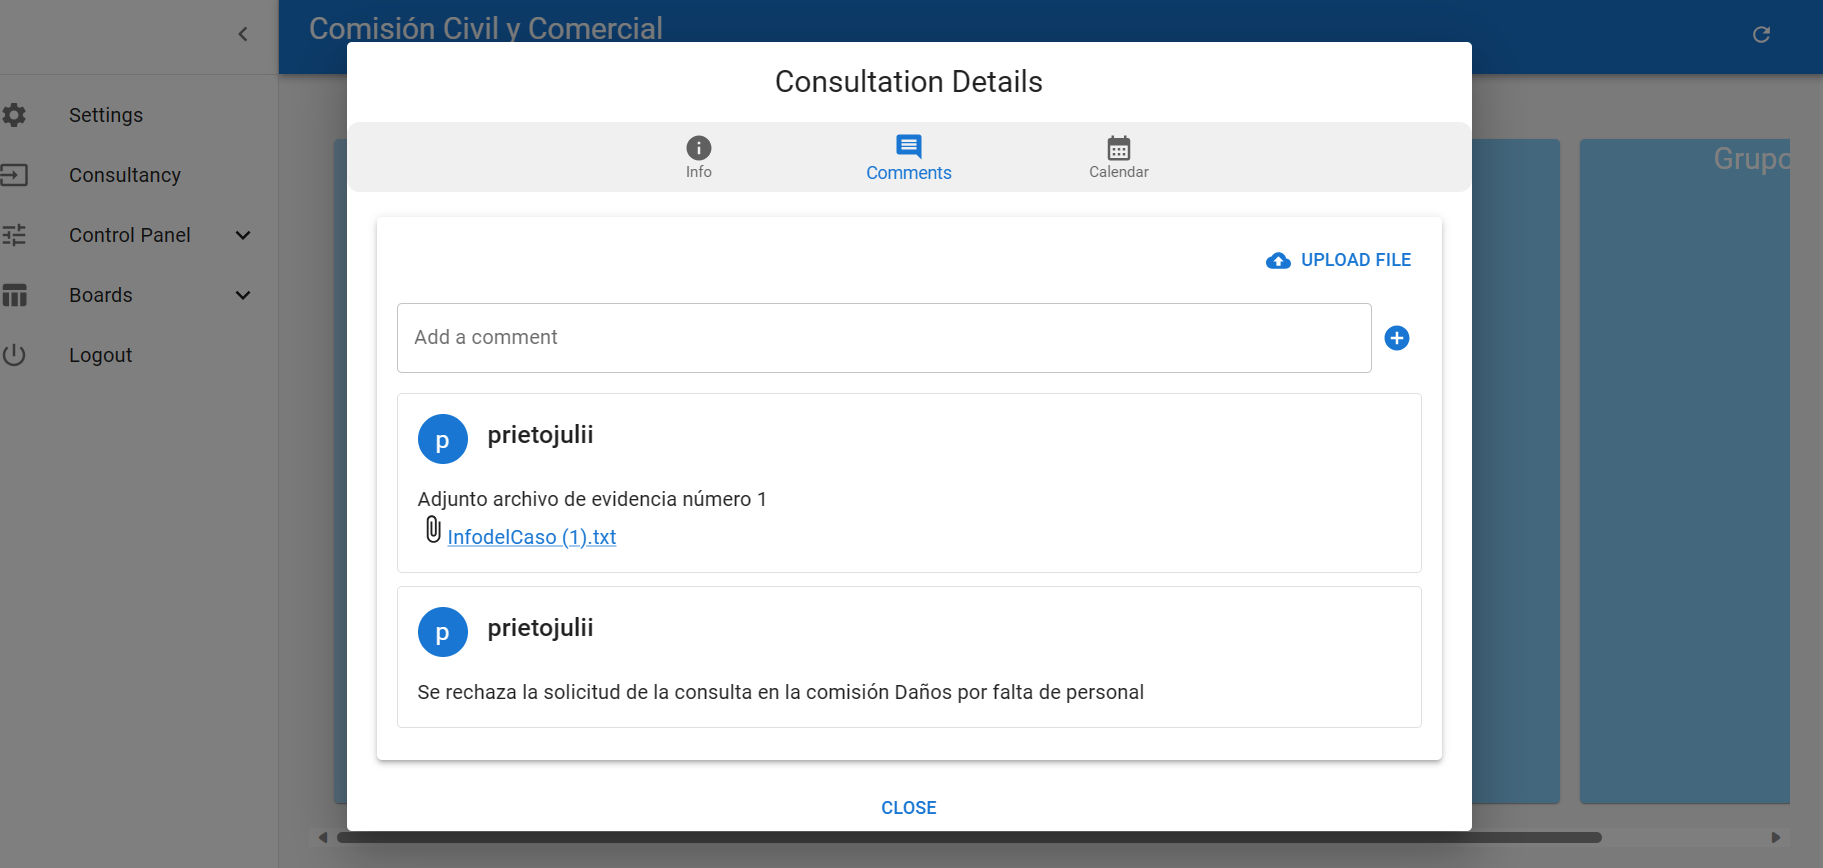
\includegraphics[width=1\linewidth]{fig/comentario-consulta.png}
    \caption{Sección de Comentarios y Archivos.}
    \label{fig:consulta-comentarios}
\end{figure}

La segunda pestaña es una sección dedicada para registrar comentarios y archivos relevantes que contribuyan al seguimiento del caso.

\begin{figure}[H]
    \centering
    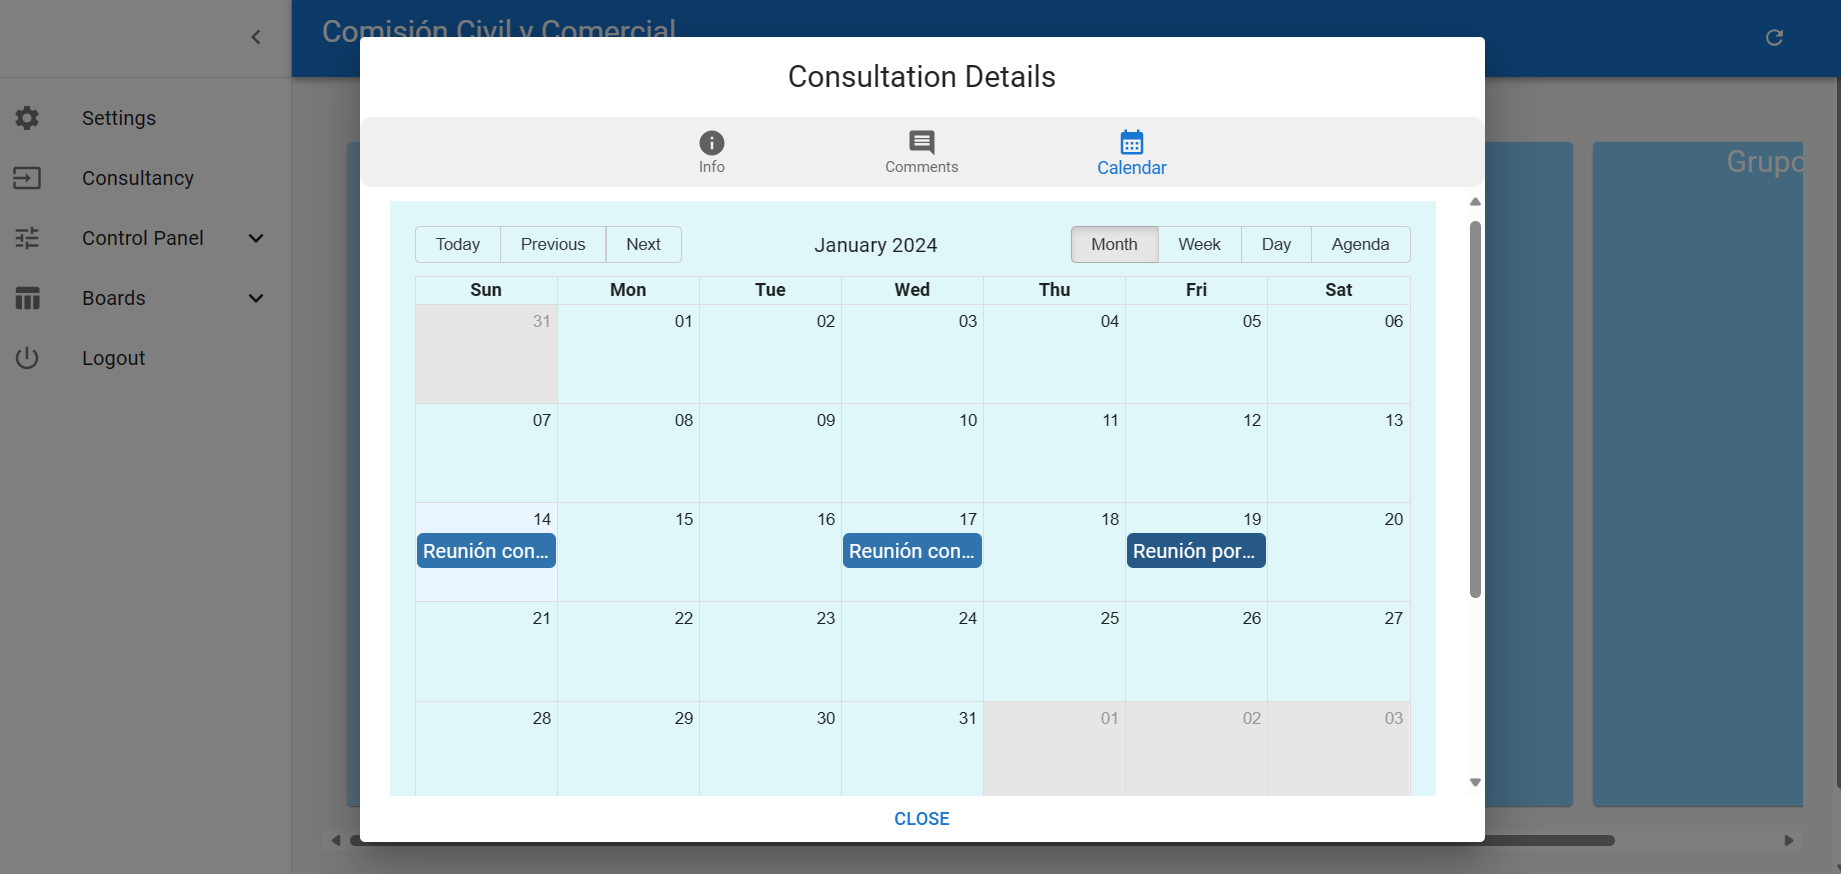
\includegraphics[width=1\linewidth]{fig/consulta-calendar-1.png}
    \caption{Calendario de Consulta.}
    \label{fig:consulta-calendar-1}
\end{figure}

La tercera ventana es un calendario que permite registrar eventos relacionados con el caso, como reuniones o fechas importantes.

\begin{figure}[H]
    \centering
    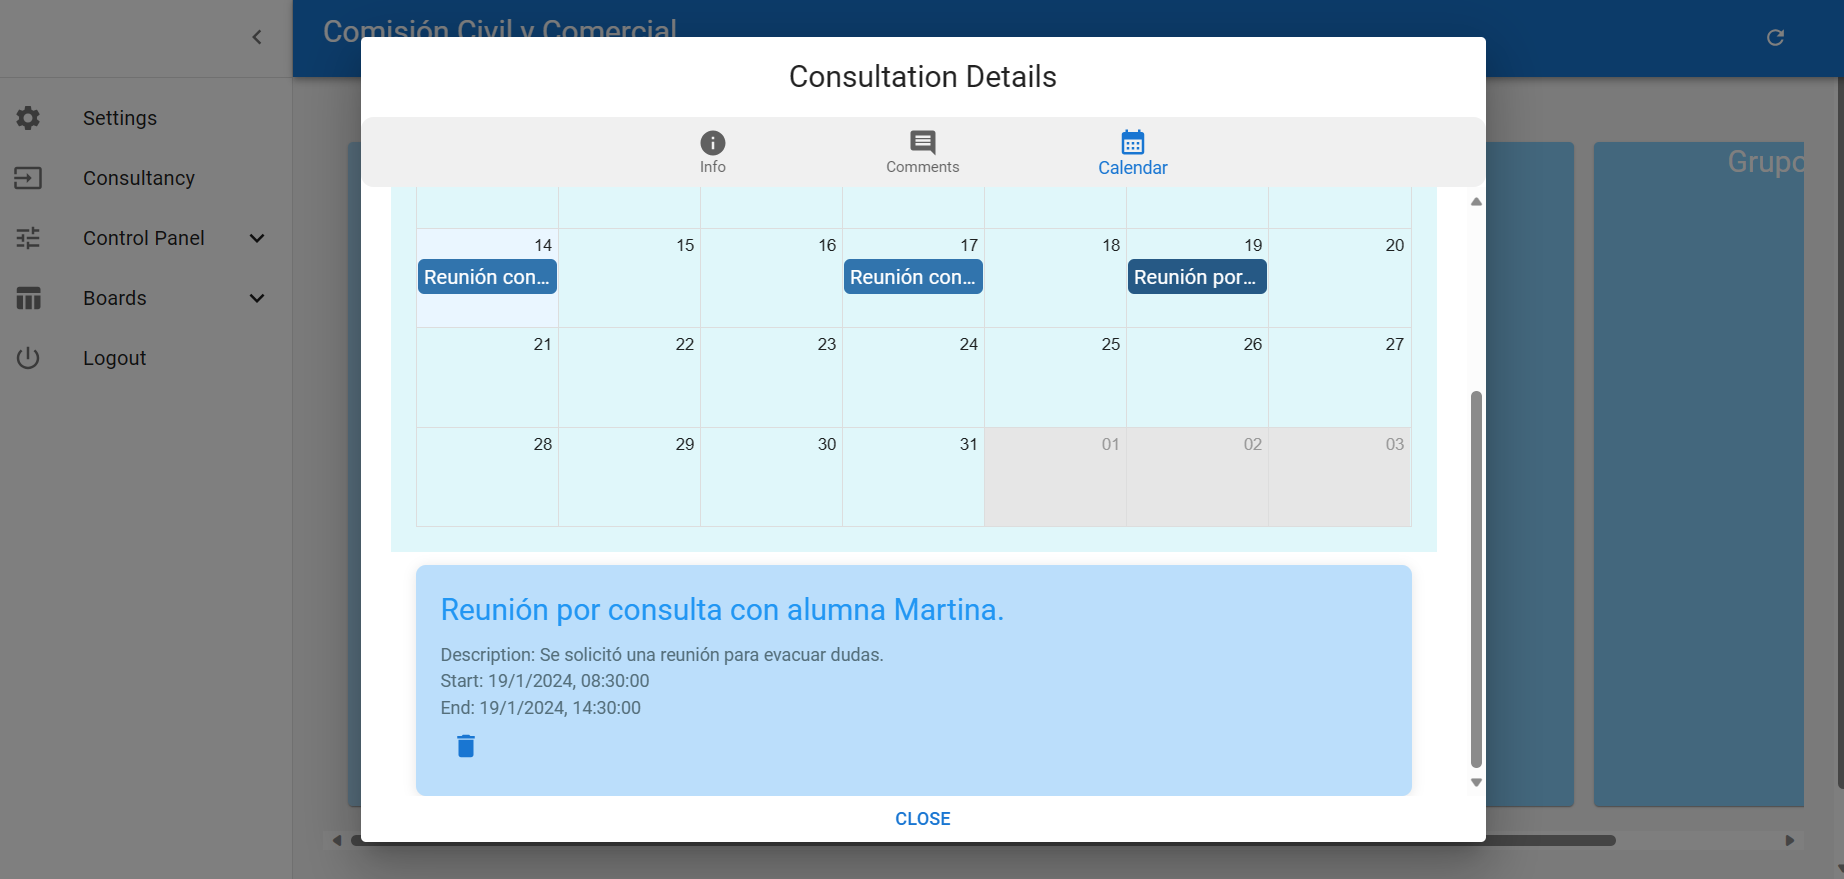
\includegraphics[width=1\linewidth]{fig/consulta-calendar-2.png}
    \caption{Detalle de Evento del Calendario de Consulta.}
    \label{fig:consulta-calendar-2}
\end{figure}
Al seleccionar un evento en el calendario, se desplegará una vista detallada con información adicional.

\begin{figure}[H]
    \centering
    \includegraphics[width=1\linewidth]{fig/consulta-calendar-3.png}
    \caption{Vista Agenda de Calendario de Consulta.}
    \label{fig:consulta-calendar-3}
\end{figure}

Este calendario ofrece varias vistas, como mensual, semanal, diaria o en formato de agenda, según se visualiza en la imagen anterior. Es una herramienta clave para organizar y dar seguimiento a eventos relevantes asociados a la consulta.

\section{Configuración de Cuenta}\label{sec:configuracion-cuenta}

La sección de configuración de cuenta, accesible desde la página de ``Settings'', proporciona la capacidad de visualizar y editar información personalizada, como el nombre de usuario y la contraseña.

\begin{figure}[H]
    \centering
    \includegraphics[width=1\linewidth]{fig/settings-real-page.png}
    \caption{Página de Configuración de Cuenta.}
    \label{fig:settings-page}
\end{figure}

    \chapter{Conclusiones}\label{cap:conclusiones}

Durante el desarrollo de este proyecto, me enfrenté a diversos desafíos que impulsaron la expansión de mis conocimientos en diferentes frameworks y lenguajes de programación. La inmersión en el paradigma de programación funcional al trabajar con React proporcionó una perspectiva declarativa que enriqueció mi capacidad para abordar problemas de manera diferente.

Este año no solo significó la adquisición de nuevas habilidades técnicas, sino también el perfeccionamiento de buenas prácticas y la exploración de nuevas tecnologías, así como la gestión de proyectos y la relación con el cliente. La experiencia en el desarrollo del Sistema de Gestión de Casos no solo amplió mi comprensión teórica, sino que también me permitió aplicar esos conocimientos participando en todas las fases del proyecto.

El desarrollo e implementación del Sistema de Gestión de Casos (Case Management System) representa un hito significativo en el ámbito del patrocinio jurídico, proporcionando una solución tecnológica adaptable a las necesidades específicas del laboratorio IALAB de la Universidad de Buenos Aires. A lo largo de este proceso, se han alcanzado varios objetivos clave que abarcan desde la automatización de la captura de consultas hasta la gestión eficiente de los casos y su asignación a comisiones especializadas.

En primer lugar, la integración con Google Forms estableció un canal eficaz para la recepción de consultas. La aplicación de estrategias y scripts personalizados en Google Forms superó desafíos como la limitación de tipos de datos, facilitando la gestión de preguntas interdependientes y proporcionando una interfaz intuitiva para la gestión de credenciales.

La arquitectura modular y la implementación de tecnologías como Django, React y Docker impulsaron la escalabilidad y el mantenimiento del sistema. La adopción de buenas prácticas en el desarrollo, como la estructuración modular del backend y frontend, el uso de contenedores para la implementación y la aplicación de patrones de diseño como el Pub/Sub, contribuyó a la solidez y flexibilidad del sistema.

La creación de un tablero de trabajo para la consultoría resultó instrumental para la toma de decisiones y el seguimiento de asignaciones. La capacidad de arrastrar y soltar consultas, la visualización detallada del historial de asignaciones y los comentarios y calendarios de las consultas optimizaron la eficiencia, trazabilidad y el control en la gestión de casos.

En cuanto a la seguridad, la implementación de roles específicos y la creación de un mecanismo de autorización fortalecieron la protección de datos y la administración de credenciales, asegurando la confidencialidad e integridad de la información sensible.

El sistema sienta las bases para un sistema modular que ofrece flexibilidad para un proceso continuo que seguirá en desarrollo. En futuras versiones, se explorarán oportunidades de mejora, como fortalecer la integración con Google Forms para permitir la edición de datos de consultantes y consultas después de su envío inicial, realización de informes y estadísticas, como la clasificación de los casos por categorías, y la integración de filtros automáticos para asistir a los tomadores de casos en el Patrocinio Jurídico de la Universidad de Buenos Aires.
    \appendix
    \chapter{Matriz de Relaciones}\label{cap:apendix-matrix-relation}

En esta sección, se presenta la matriz de relaciones, una herramienta utilizada para el diseño de la base de datos del sistema. La matriz de relaciones permite visualizar y comprender las interconexiones entre las diversas entidades que componen la estructura de la base de datos.

El objetivo fundamental de este análisis es identificar y descubrir las relaciones entre las entidades, proporcionando una visión clara de cómo interactúan y se relacionan unos con otros.

A lo largo de la matriz, se representan las relaciones entre entidades específicas, asignándoles significado y nombres a estas conexiones. Cada celda de la matriz detalla cómo las instancias de una entidad están relacionadas con las instancias de otra entidad, y se proporciona una descripción contextual que ayuda a comprender la naturaleza de la conexión entre ellas.

La información contenida en la matriz de relaciones se deriva de un proceso de modelado y refinamiento continuo hasta alcanzar la tercera forma normal, un estándar en la normalización de bases de datos que promueve la eficiencia y evita redundancias.


\begin{sidewaystable}[p]
    \centering
        \begin{tabular}{|p{4.1cm}|*{6}{>{\raggedright\arraybackslash}p{2.5cm}|}}
         \hline
         & \textbf{Calendar} & \textbf{Event} & \textbf{Card} & \textbf{Panel} & \textbf{Board} & \textbf{Request} \textbf{Consultation} \\
         \hline
        \textbf{Calendar} & \cellcolor{gray!25} & Contiene & Contenido en & x & x & x \\
         \hline
        \textbf{Event} & Contenido en & \cellcolor{gray!25} & x & x & x & x \\
         \hline
        \textbf{Card} & Tiene un & x & \cellcolor{gray!25} & Contenida en & x & x  \\
         \hline
        \textbf{Panel} & x & x & Contiene & \cellcolor{gray!25} & Contenido en & x \\
         \hline
        \textbf{Board} & x & x & x & Tiene & \cellcolor{gray!25} &   Le llegan\\
         \hline
        \textbf{RequestConsultation} & x & x & x & x & Hacia un & \cellcolor{gray!25} \\
         \hline
        \textbf{Consultation} & x & x & Tiene una & x & x & Tiene \\
         \hline
        \textbf{Client} & x & x & x & x & x & x  \\
         \hline
        \textbf{Patrimony} & x & x & x & x & x & x  \\
         \hline
        \textbf{Tel} & x & x & x & x & x & x \\
         \hline
        \textbf{User} & x & x & x & x & Miembro de & x \\
         \hline
        \textbf{Comment} & x & x & Está en una & x & x & x \\
         \hline
        \textbf{File} & x & x & x & x & x & x  \\
         \hline
        \textbf{Family} & x & x & x & x & x & x  \\
         \hline
        \textbf{Locality} & x & x & x & x & x & x  \\
         \hline
        \textbf{Province} & x & x & x & x & x & x  \\
         \hline
        \textbf{Nationality} & x & x & x & x & x & x  \\
         \hline
        \textbf{Child} & x & x & x & x & x & x  \\
         \hline
        \end{tabular})
        \caption{Matriz de Relaciones Primera Parte}
        \label{mat:der}
        \end{sidewaystable}


        
\begin{sidewaystable}[p]
    \centering
        \begin{tabular}{|p{4.1cm}|*{7}{>{\raggedright\arraybackslash}p{2.5cm}|}}
         \hline
         & \textbf{Consultation} & \textbf{Client} & \textbf{Patrimony} & \textbf{Tel} & \textbf{User} & \textbf{Comment} & \textbf{File} \\
         \hline
        \textbf{Calendar} & x & x & x & x & x & x & x \\
         \hline
        \textbf{Event} & x & x & x & x & x & x & x \\
         \hline
        \textbf{Card}  & Pertenece a & x & x & x & x & x & x \\
         \hline
        \textbf{Panel}  & x & x & x & x & x & x & x \\
         \hline
        \textbf{Board}  & x & x & x & x & Tiene Miembros & x & x \\
         \hline
        \textbf{RequestConsultation} &  Solicita enviar una & x & x & x & x & x & x \\
         \hline
        \textbf{Consultation} & \cellcolor{gray!25} & Realizada por & x & x & x & Tiene & x \\
         \hline
        \textbf{Client}  & Realiza una & \cellcolor{gray!25} & Tiene & Tiene & x & x & x \\
         \hline
        \textbf{Patrimony}  & x & Pertenece a & \cellcolor{gray!25} & x & x & x & x \\
         \hline
        \textbf{Tel}  & x & Pertenece a & x & \cellcolor{gray!25} & x & &   \\
         \hline
        \textbf{User} & x & x & x & x & \cellcolor{gray!25} & Realiza un & x \\
         \hline
        \textbf{Comment}  & x & x & x & x & Lo comenta & \cellcolor{gray!25} & Tiene \\
         \hline
        \textbf{File}  & & & x & x & x & Adjuntado en & \cellcolor{gray!25}\\
         \hline
        \textbf{Family}  & x & Es de un & x & x & x & x & x \\
         \hline
        \textbf{Locality} & x & Residida por & x & x & x & x & x \\
         \hline
        \textbf{Province} & x & x & x & x & x & x & x \\
         \hline
        \textbf{Nationality} & x & x & x & x & x & x & x \\
         \hline
        \textbf{Child}  & x & x & x & x & x & x & x \\
         \hline
        \end{tabular})
        \caption{Matriz de Relaciones Segunda Parte}
        \label{mat:der2}
        \end{sidewaystable}


        
\begin{sidewaystable}[p]
    \centering
        \begin{tabular}{|p{4.1cm}|*{5}{>{\raggedright\arraybackslash}p{2.5cm}|}}
         \hline
       & \textbf{Family} & \textbf{Locality} & \textbf{Province} & \textbf{Nationality} & \textbf{Child} \\
         \hline
        \textbf{Calendar} & x & x & x & x & x \\
         \hline
        \textbf{Event} & x & x & x & x & x \\
         \hline
        \textbf{Card}  & x & x & x & x & x \\
         \hline
        \textbf{Panel}  & x & x & x & x & x \\
         \hline
        \textbf{Board}  & x & x & x & x & x \\
         \hline
        \textbf{RequestConsultation} & x & x & x & x & x \\
         \hline
        \textbf{Consultation}  & x & x & x & x & x \\
         \hline
        \textbf{Client} & Tiene una & Reside en & x & x & x \\
         \hline
        \textbf{Patrimony}  & x & x & x & x & x \\
         \hline
        \textbf{Tel}  & x & x & x & x & \\
         \hline
        \textbf{User}  & x & x & x & x & x  \\
         \hline
        \textbf{Comment}  & x & x & x & x & x \\
         \hline
        \textbf{File} & x & x & x & x & x \\
         \hline
        \textbf{Family}  & \cellcolor{gray!25} & x & x & x & Contiene \\
         \hline
        \textbf{Locality} & x & \cellcolor{gray!25} & Está en & x & Residida por \\
         \hline
        \textbf{Province}  & x & Tiene & \cellcolor{gray!25} & Está en & x \\
         \hline
        \textbf{Nationality}  & x & x & Tiene & \cellcolor{gray!25} & x \\
         \hline
        \textbf{Child}  & Está en una & Reside en & x & x & \cellcolor{gray!25} \\
         \hline
        \end{tabular})
        \caption{Matriz de Relaciones Tercera Parte}
        \label{mat:der3}
        \end{sidewaystable}

    \chapter{Configuración de Nginx}\label{cap:apendix-nginx}
% Configuración de estilo para el código
\lstset{
    language=sh,
    backgroundcolor=\color{white},
    basicstyle=\footnotesize\ttfamily,
    keywordstyle=\color{blue},
    commentstyle=\color{green},
    stringstyle=\color{red},
    captionpos=b,
    breaklines=true,
    showstringspaces=false,
    numbers=left,
    numberstyle=\tiny,
    frame=single,
    rulecolor=\color{black}
}

\section{Configuración del Ngnix como Reverse Proxy}\label{subsec:nginx_explicacion}
El archivo de configuración Nginx utilizado como proxy reverse en el Stack de contenedores es el siguiente:
\begin{lstlisting}[caption={Configuración de Nginx Reverse Proxy}, label={cod:nginx}, captionpos=b]
limit_conn_zone $binary_remote_addr zone=addr:10m;

upstream gunicorn{
    server appserver:8000;
}

upstream daphne{
    server appserver:8001;
}

upstream frontend{
    server frontend:3000;
}

server {
    client_body_timeout 5s;
    client_header_timeout 5s; # Closing Slow Connections
    server_tokens off;
    listen 80;
    listen  [::]:80;
    server_name  proyecto-patrocinio.fcefyn.unc.edu.ar;

    location / {
        limit_req zone=mylimit burst=20 nodelay;
        limit_conn addr 10;
        try_files $uri @proxy_frontend;
    }
    location /api {
        limit_req zone=mylimit burst=20 nodelay;
        limit_conn addr 10;
        try_files $uri @proxy_api_wsgi;
    }
    location /ws {
        limit_req zone=mylimit burst=20 nodelay;
        limit_conn addr 10;
        try_files $uri @proxy_api_asgi;
    }
    location /admin {
        limit_req zone=mylimit burst=20 nodelay;
        limit_conn addr 10;
        root /usr/src/app/django_static;
        include /etc/nginx/mime.types;
        try_files $uri @proxy_api_wsgi;
    }

    # redirect to django app: React server
    location @proxy_frontend {
        proxy_pass http://frontend;
        proxy_redirect off;
        proxy_cache_bypass  $http_upgrade;
        proxy_set_header Upgrade           $http_upgrade;
        proxy_set_header Connection        "upgrade";
        proxy_set_header Host              $host;
        proxy_set_header X-Real-IP         $remote_addr;
        proxy_set_header X-Forwarded-For   $proxy_add_x_forwarded_for;
        proxy_set_header X-Forwarded-Proto $scheme;
        proxy_set_header X-Forwarded-Host  $host;
        proxy_set_header X-Forwarded-Port  $server_port;
        proxy_set_header Cookie $http_cookie;
    }

    # redirect to django app: API REST
    location @proxy_api_wsgi {
        proxy_pass http://gunicorn;
        proxy_redirect off;
        proxy_cache_bypass  $http_upgrade;
        proxy_set_header Upgrade           $http_upgrade;
        proxy_set_header Connection        "upgrade";
        proxy_set_header Host              $host;
        proxy_set_header X-Real-IP         $remote_addr;
        proxy_set_header X-Forwarded-For   $proxy_add_x_forwarded_for;
        proxy_set_header X-Forwarded-Proto $scheme;
        proxy_set_header X-Forwarded-Host  $host;
        proxy_set_header X-Forwarded-Port  $server_port;
        proxy_set_header Cookie $http_cookie;
    }

    # redirect to django app with WebSocket
    location @proxy_api_asgi {
        proxy_pass http://daphne;
        proxy_redirect off;
        proxy_cache_bypass  $http_upgrade;
        proxy_set_header Upgrade           $http_upgrade;
        proxy_set_header Connection        "upgrade";
        proxy_set_header Host              $host;
        proxy_set_header X-Real-IP         $remote_addr;
        proxy_set_header X-Forwarded-For   $proxy_add_x_forwarded_for;
        proxy_set_header X-Forwarded-Proto $scheme;
        proxy_set_header X-Forwarded-Host  $host;
        proxy_set_header X-Forwarded-Port  $server_port;
        proxy_set_header Cookie $http_cookie;
    }

    location /django_static/ {
        limit_req zone=mylimit burst=20 nodelay;
        limit_conn addr 10;
        autoindex on;
        alias /usr/share/nginx/staticfiles/cms/django/;
    }
}
\end{lstlisting}







\section{Configuración del Ngnix como Servidor}

Por otro lado, el servidor contaba con un Servidor Nginx instalado y en funcionamiento sirviendo otras aplicaciones.
Para agregar el servicio Case Managment System se agregó el siguiente archivo en el directorio \textbf{etc/nginx/conf.d/proyecto-patrocinio.fcefyn.unc.edu.ar.conf}:



\begin{lstlisting}[caption={Configuración de Nginx en el Servidor}, label={cod:nginx}, captionpos=b]

server {
    server_name proyecto-patrocinio.fcefyn.unc.edu.ar;

    location / {
        proxy_pass http://localhost:8081;
        proxy_redirect off;
        proxy_cache_bypass  $http_upgrade;
        proxy_set_header Upgrade           $http_upgrade;
        proxy_set_header Connection        "upgrade";
        proxy_set_header Host              $host;
        proxy_set_header X-Real-IP         $remote_addr;
        proxy_set_header X-Forwarded-For   $proxy_add_x_forwarded_for;
        proxy_set_header X-Forwarded-Proto $scheme;
        proxy_set_header X-Forwarded-Host  $host;
        proxy_set_header X-Forwarded-Port  $server_port;
        proxy_set_header Cookie $http_cookie;
    }

    listen 443 ssl; # managed by Certbot
    ssl_certificate /etc/letsencrypt/live/proyecto-patrocinio.fcefyn.unc.edu.ar/fullchain.pem; # managed by Certbot
    ssl_certificate_key /etc/letsencrypt/live/proyecto-patrocinio.fcefyn.unc.edu.ar/privkey.pem; # managed by Certbot
    include /etc/letsencrypt/options-ssl-nginx.conf; # managed by Certbot
    ssl_dhparam /etc/letsencrypt/ssl-dhparams.pem; # managed by Certbot

}

server {
    if ($host = proyecto-patrocinio.fcefyn.unc.edu.ar) {
        return 301 https://$host$request_uri;
    } # managed by Certbot


    listen 80;
    server_name proyecto-patrocinio.fcefyn.unc.edu.ar;
    return 404; # managed by Certbot


}
\end{lstlisting}
    \chapter{Endpoints de Formularios}\label{cap:anexo-expoint-forms}

\section{Endpoint del Formulario Registro de Cliente}

\subsection*{URL}
\texttt{http://\{\{ip\}\}:\{\{port\}\}/api/clients/client/form/}

\subsection*{Método}
POST

\subsection*{Body de Ejemplo:}
A continuación se presenta un ejemplo.
\begin{lstlisting}[caption=Body de Ejemplo, label=example-body]
{
    "first_name": "Martina",
    "last_name": "Gutierrez",
    "id_type": "DOCUMENT",
    "id_value": "42304328",
    "birth_date": "2000-11-13",
    "sex": "FEMALE",
    "marital_status": "SINGLE",
    "studies": "INCOMPLETE_UNIVERSITY",
    "email": "martina2000@gmail.com",
    "housing_type": "HOUSE",
    "locality": 9,
    "address": "Av. Patria 1234",
    "postal": "5000",
    "employment": "programmer",
    "salary": "123",
    "other_income": "No tengo otros ingresos",
    "amount_other_income": "0",
    "amount_retirement": "0",
    "amount_pension": "0",
    "vehicle": "No tengo otros vehiculos",
    "tel": [
        "3512254210",
        "+54 9 25578784"
    ],
    "partner_salary": "0"
}
\end{lstlisting}
\subsection*{Campos del Body:}

\begin{table}[H]
    \centering
    \begin{tabular}{|l|l|p{5cm}|p{5cm}|}
        \hline
        \textbf{Campo} & \textbf{Tipo} & \textbf{Opciones} & \textbf{Descripción} \\ \hline
        first\_name & String & & Nombre del consultante. \\ \hline
        last\_name & String & & Apellido del consultante. \\ \hline
        id\_type & String & DOCUMENT, PASSPORT & Tipo de documento de identidad. \\ \hline
        id\_value & String & & Valor del documento de identidad. \\ \hline
        birth\_date & String & & Fecha de nacimiento del consultante. \\ \hline
        sex & String & MALE, FEMALE & Género del consultante. \\ \hline
        marital\_status & String & SINGLE, MARRIED, DIVORCED, WIDOWER & Estado civil del consultante. \\ \hline
        studies & String & INCOMPLETE\_PRIMARY, COMPLETE\_PRIMARY, INCOMPLETE\_SECONDARY, COMPLETE\_SECONDARY, INCOMPLETE\_TERTIARY, COMPLETE\_TERTIARY, INCOMPLETE\_UNIVERSITY, COMPLETE\_UNIVERSITY & Nivel de estudios del consultante. \\ \hline
        email & String & & Correo electrónico del consultante. \\ \hline
        housing\_type & String & HOUSE, DEPARTMENT, TRAILER, STREET\_SITUATION & Tipo de vivienda del consultante. \\ \hline
        locality & Integer & & ID de localidad del consultante. \\ \hline
        address & String & & Dirección del consultante. \\ \hline
        postal & String & & Código postal del consultante. \\ \hline
        employment & String & & Ocupación del consultante. \\ \hline
        salary & String & & Salario del consultante. \\ \hline
        other\_income & String & & Otros ingresos del consultante. \\ \hline
        amount\_other\_income & String & & Monto de otros ingresos. \\ \hline
        amount\_retirement & String & & Monto de jubilación. \\ \hline
        amount\_pension & String & & Monto de pensión. \\ \hline
        vehicle & String & & Información sobre vehículos del consultante. \\ \hline
        tel & List & & Lista de números de teléfono del consultante. \\ \hline
        partner\_salary & String & & Salario del cónyuge (si aplica). \\ \hline
    \end{tabular}
    \caption{Descripción de campos del Body}
    \label{tab:body-fields-client}
\end{table}


\subsection*{Headers:}

\begin{itemize}
    \item \textbf{Authorization:} Token \{\{TOKEN\}\}
    \item \textbf{Content-Type:} application/json
\end{itemize}






\section{Endpoint del Formulario Registro de Hijo}

\subsection*{URL}
\texttt{http://\{\{ip\}\}:\{\{port\}\}/api/clients/son/form/}

\subsection*{Método}
POST

\subsection*{Campos del Body:}

\begin{table}[H]
    \centering
    \begin{tabular}{|l|l|l|p{7cm}|}
        \hline
        \textbf{Campo} & \textbf{Tipo} & \textbf{Opciones} & \textbf{Descripción} \\ \hline
        id\_consultant & String & & Identificación del consultor asociado. \\ \hline
        first\_name & String & & Nombre del hijo. \\ \hline
        last\_name & String & & Apellido del hijo. \\ \hline
        id\_type & String & DOCUMENT, PASSPORT & Tipo de documento de identidad del hijo. \\ \hline
        id\_value & String & & Valor del documento de identidad del hijo. \\ \hline
        birth\_date & String & & Fecha de nacimiento del hijo. \\ \hline
        sex & String & MALE, FEMALE & Género del hijo. \\ \hline
        locality & Integer & & ID de la localidad del hijo. \\ \hline
        address & String & & Dirección del hijo. \\ \hline
    \end{tabular}
    \caption{Descripción de campos del Body}
    \label{tab:body-fields-son}
\end{table}

\newpage
\subsection*{Body de Ejemplo:}

\begin{lstlisting}[caption=Body de Ejemplo, label=example-body-son]
{
    "id_consultant": "42304328",
    "first_name": "Matilda",
    "last_name": "Gonzales",
    "id_type": "PASSPORT",
    "id_value": "123456789",
    "birth_date": "2020-11-14",
    "sex": "FEMALE",
    "locality": 9,
    "address": "Av. Patria 1234"
}
\end{lstlisting}


\subsection*{Headers:}

\begin{itemize}
    \item \textbf{Authorization:} Token \{\{TOKEN\}\}
    \item \textbf{Content-Type:} application/json
\end{itemize}




\section{Endpoint del Formulario Consulta}

\subsection*{URL}
\texttt{http://\{\{ip\}\}:\{\{port\}\}/api/consultations/consultation/form/}

\subsection*{Método}
POST

\subsection*{Body de Ejemplo:}

\begin{lstlisting}[caption=Body de Ejemplo, label=example-body-consultation]
{
    "client": "42304328",
    "tag": "Asesoramiento Legal",
    "description": "Necesito asesoramiento legal con respecto a una disputa contractual con la Corporacion XYZ. El contrato involucra la venta de bienes y hay desacuerdos sobre los plazos de entrega y los terminos de pago.",
    "opponent": "Corporacion XYZ"
}
\end{lstlisting}

\subsection*{Campos del Body:}

\begin{table}[H]
    \centering
    \begin{tabular}{|l|l|l|p{7cm}|}
        \hline
        \textbf{Campo} & \textbf{Tipo} & \textbf{Opciones} & \textbf{Descripción} \\ \hline
        client & String & & Identificación del consultante asociado a la consulta. \\ \hline
        tag & String & & Etiqueta de la consulta. \\ \hline
        description & String & & Descripción detallada de la consulta. \\ \hline
        opponent & String & & Oponente o entidad involucrada en la consulta. \\ \hline
    \end{tabular}
    \caption{Descripción de campos del Body}
    \label{tab:body-fields-consultation}
\end{table}

\subsection*{Headers:}

\begin{itemize}
    \item \textbf{Authorization:} Token \{\{TOKEN\}\}
    \item \textbf{Content-Type:} application/json
\end{itemize}

    \chapter{Archivos de Configuración para el Despliegue de la Plataforma}\label{cap:apendix-configfile-deloy}
\lstset{
    language=sh,
    backgroundcolor=\color{white},
    basicstyle=\footnotesize\ttfamily,
    keywordstyle=\color{blue},
    commentstyle=\color{green},
    stringstyle=\color{red},
    captionpos=b,
    breaklines=true,
    showstringspaces=false,
    numbers=left,
    numberstyle=\tiny,
    frame=single,
    rulecolor=\color{black}
}

\section{Archivo de configuración \textbf{.env}}\label{sec:anexo:configfile-env}
Archivo de configuración de variables de entorno usadas por \textit{docker-compose.yml}.
\begin{lstlisting}[caption={Archivo de configuración .env}, label={cod:.env}, captionpos=b]
CMS_BACKEND_IMAGE=proyectopatrocinio/backend-patrocinio:v1.0.0
CMS_FRONTEND_IMAGE=proyectopatrocinio/frontend-patrocinio:v1.0.0
CMS_PROXY_PORT=8081
CMS_NGINX_CONFIG_FILE=./resources/nginx.conf
CMS_BACKEND_ENV_FILE=./resources/backend.env
CMS_POSTGRES_ENV_FILE=./resources/postgres.env
CMS_FRONTEND_ENV_FILE=./resources/frontend.env
CMS_TEMPLATES_ACCOUNT_PATH=./resources/templates/account/
CMS_TEMPLATES_NOTIFICATION_PATH=./resources/templates/notifications/
CMS_TERMS_AND_POLICIES_FILE=./resources/terms_and_policies.md
\end{lstlisting}



\section{Archivo de configuración \textbf{backend.env}}\label{sec:anexo:configfile-backend-env}
Archivo de configuración de variables de entorno del servicio backend para el deploy de Docker Swarm:

\begin{lstlisting}[caption={Archivo de configuración backend.env}, label={cod:backend.env}, captionpos=b]
DEBUG=0
DJANGO_ALLOWED_HOSTS=proyecto-patrocinio.fcefyn.unc.edu.ar databaseserver nginxserver appserver redis_server frontend
SQL_ENGINE=django.db.backends.postgresql
SQL_DATABASE=patrocinio_prod
SQL_USER=patrocinio_api
SQL_PASSWORD=****
SQL_HOST=db
SQL_PORT=5432
DATABASE=postgres
EMAIL_HOST_USER=*****
EMAIL_HOST_PASSWORD=******
CORS_ALLOWED_ORIGINS=http://nginx:80 http://frontend:3000
HOSTNAME=proyecto-patrocinio.fcefyn.unc.edu.ar
CONSULTANCY_BOARD_NAME=CONSULTORIA
DEFAULT_HTTP_PROTOCOL=https
CSRF_TRUSTED_ORIGINS=http://nginx:80 http://frontend:3000 https://proyecto-patrocinio.fcefyn.unc.edu.ar
LOG_ROTATE_DAYS=10
SECRET_KEY=****
DJANGO_SUPERUSER_USERNAME=*****
DJANGO_SUPERUSER_PASSWORD=*****
DJANGO_SUPERUSER_EMAIL=****
\end{lstlisting}


\section{Archivo de configuración \textbf{frontend.env}}\label{sec:anexo:configfile-frontend-env}
Archivo de configuración de variables de entorno del servicio frontend para el deploy de Docker Swarm:

\begin{lstlisting}[caption={Archivo de Configuración frontend.env}, label={cod:frontend.env}, captionpos=b]
# Utilizar el dominio correspondiente
REACT_APP_URL_BASE_API_REST_PATROCINIO=https://proyecto-patrocinio.fcefyn.unc.edu.ar/api/
REACT_APP_WS_NOTIFICATION_PATH_PATROCINIO=wss://proyecto-patrocinio.fcefyn.unc.edu.ar/ws/notification/

# No cambiar las siguientes variables
REACT_APP_PATH_TERMS=terms/
REACT_APP_PATH_LOGIN=auth/login/
REACT_APP_PATH_LOGOUT=auth/logout/
REACT_APP_PATH_RESET_PASSWORD=auth/password/reset/
REACT_APP_PATH_RESET_PASSWORD_CONFIRM=auth/password/reset-confirm/
REACT_APP_PATH_CHANGE_PASSWORD=auth/password/change/
REACT_APP_PATH_USER=auth/user/
REACT_APP_PATH_USER_BY_TOKEN=auth/user-by-token/?token=
REACT_APP_PATH_RESEND_EMAIL=auth/resend-email/
REACT_APP_PATH_SIGNUP=register/
REACT_APP_PATH_USERBOARD=boardusers/boarduser/
REACT_APP_PATH_USERBOARD_BY_USER=boardusers/boarduser/?user_id=
REACT_APP_PATH_CARDS=cards/card/
REACT_APP_PATH_CONSULTATIONS=consultations/consultation/
REACT_APP_PATH_FILTER_CONSULTATIONS_BY_AVAILABILITY=consultations/consultation/?availability_state=
REACT_APP_PATH_REQUEST_CARDS=consultations/request_consultation/
REACT_APP_EXTRA_PATH_ACCEPT_REQUEST_CARDS=/accepted/
REACT_APP_EXTRA_PATH_REJECTED_REQUEST_CARDS=/rejected/
REACT_APP_PATH_BOARD=boards/board/
REACT_APP_PATH_REQUEST_CONSULTANCY_BOARD=boards/board/consultancy_board/
REACT_APP_EXTRA_PATH_BOARD_LOGS=/logs/?days=
REACT_APP_PATH_PANELS=panels/panel/
REACT_APP_PATH_CLIENTS=clients/client/
REACT_APP_PATH_TEL=clients/tel/
REACT_APP_PATH_PATRIMONY=clients/patrimony/
REACT_APP_PATH_FAMILY=clients/family/
REACT_APP_PATH_CHILDREN=clients/child/
REACT_APP_PATH_LOCALITY=geography/locality/
REACT_APP_PATH_PROVINCE=geography/province/
REACT_APP_PATH_NATIONALITY=geography/nationality/
REACT_APP_PATH_COMMENTS=comments/comment/
REACT_APP_PATH_COMMENTS_BY_CONSULT=comments/comment/?consultation_id=
REACT_APP_PATH_ATTACH_COMMENT_FILE=comments/file/
REACT_APP_PATH_CALENDAR=calendars/calendar/
REACT_APP_PATH_CALENDAR_EVENT=calendars/event/
\end{lstlisting}



\section{Archivo de configuración \textbf{portgres.env}}\label{sec:anexo:configfile-portgres-env}
Archivo de configuración de variables de entorno de la base de datos para el deploy de Docker Swarm:

\begin{lstlisting}[caption={Archivo de configuración portgres.env}, label={cod:portgres.env}, captionpos=b]
POSTGRES_DB=patrocinio_prod
POSTGRES_USER=patrocinio_api
PGDATA=/var/lib/postgresql/data
POSTGRES_PASSWORD=*****

\end{lstlisting}
    \chapter{Test Unitarios}\label{cap:apendix-unitest}
% Configuración de estilo para el código
\lstset{
    language=python,
    backgroundcolor=\color{white},
    basicstyle=\footnotesize\ttfamily,
    keywordstyle=\color{blue},
    commentstyle=\color{green},
    stringstyle=\color{red},
    captionpos=b,
    breaklines=true,
    showstringspaces=false,
    numbers=left,
    numberstyle=\tiny,
    frame=single,
    rulecolor=\color{black}
}

\section{Ejemplo de Test Unitario en Backend}\label{sec:apendix-unitest-1}


\begin{lstlisting}[caption={Test Unitario Backend}, label={cod:python}, captionpos=b]
class BoardUserPermissionTest(APITestCase):

    def setUp(self):
        """Set up the request factory and viewset for each test."""
        self.factory = APIRequestFactory()
        self.viewset = BoardUserViewSet.as_view({'get': 'list', 'post': 'create', 'put': 'update', 'delete': 'destroy'})
        self.url = reverse('board_user-list')
        setUpSuperUser(self)
        self.board = Board.objects.create(title='Test Board')

    def test_board_user_creation(self):
        """Test that a BoardUser instance can be created successfully."""
        board_user = BoardUser.objects.create(user=self.user, board=self.board)
        self.assertTrue(isinstance(board_user, BoardUser))
        self.assertEqual(board_user.user, self.user)
        self.assertEqual(board_user.board, self.board)

    def test_board_user_uniqueness(self):
        """Test that two instances with the same user and board cannot be created."""
        BoardUser.objects.create(user=self.user, board=self.board)
        with self.assertRaises(Exception):
            BoardUser.objects.create(user=self.user, board=self.board)

    def test_board_user_str_representation(self):
        """Test the string representation of the BoardUser object."""
        board_user = BoardUser.objects.create(user=self.user, board=self.board)
        expected_str = f'{self.user}/{self.board}'
        self.assertEqual(str(board_user), expected_str)

    def test_unauthenticated_user_cannot_access_board_users(self):
        """Test that an unauthenticated user cannot access the board users endpoint."""
        request = self.factory.get('/boardusers/')
        response = self.viewset(request)
        self.assertEqual(response.status_code, status.HTTP_403_FORBIDDEN)

    def test_authenticated_user_can_list_board_users(self):
        """Test that an authenticated user can list board users."""
        request = self.factory.get('/boardusers/')
        request.user = self.user
        response = self.viewset(request)
        self.assertEqual(response.status_code, status.HTTP_200_OK)

    def test_authenticated_user_can_create_board_user(self):
        """Test that an authenticated user can create a board user."""
        request_data = {'user': self.user.id, 'board': self.board.id}
        request = self.factory.post('/boardusers/', request_data)
        request.user = self.user
        response = self.viewset(request)
        self.assertEqual(response.status_code, status.HTTP_201_CREATED)

    def test_authenticated_user_cannot_delete_board_user(self):
        """Test that an authenticated user cannot delete a board user."""
        request = self.factory.delete('/boardusers/1/')
        response = self.viewset(request, pk=1)
        self.assertEqual(response.status_code, status.HTTP_403_FORBIDDEN)
\end{lstlisting}


\section{Ejemplo de Test Unitario en Frontend}\label{sec:apendix-unitest-2}

\begin{lstlisting}[caption={Test Unitario Frontend}, label={cod:python}, captionpos=b]
describe('ConsutationDisplay Component', () => {
  test('renders and switches between windows', async () => {
    // Render the component
    render(
      <ConsutationDisplay
        consultation={{ consultation: 1, id: 1 }}
        open={true}
        onClose={() => {}}
        updateViewTag={() => {}}
      />
    );

    expect(screen.getByText(/Consultation Details/)).toBeInTheDocument();
    expect(screen.getByText("Info")).toBeInTheDocument();
    expect(screen.getByText("Comments")).toBeInTheDocument();
    expect(screen.getByText("Calendar")).toBeInTheDocument();

    // Verify that the default window is "Info"
    expect(screen.getByTestId('info-component')).toBeInTheDocument();
    expect(screen.queryByTestId('comment-component')).toBeNull();
    expect(screen.queryByTestId('calendar-component')).toBeNull();

    // Switch to "Comments" window
    fireEvent.click(screen.getByText("Comments").closest('button'));
    expect(screen.getByTestId('comment-component')).toBeInTheDocument();
    expect(screen.queryByTestId('info-component')).toBeNull();
    expect(screen.queryByTestId('calendar-component')).toBeNull();

    // Switch to "Calendar" window
    fireEvent.click(screen.getByText('Calendar').closest('button'));
    expect(screen.getByTestId('calendar-component')).toBeInTheDocument();
    expect(screen.queryByTestId('info-component')).toBeNull();
    expect(screen.queryByTestId('comment-component')).toBeNull();

  });
});
\end{lstlisting} 

    % Bibliografía
    \bibliographystyle{plainnat}
    \bibliography{bibliografia.bib}


% Fin del documento
\end{document}
